\chapter{Work Environments}

Block programming languages are a specific category within visual programming languages. Their key characteristic is that program instructions are represented as colored blocks rather than the traditional text-based commands in classical programming languages. The primary objective of block languages is to make programming more accessible to beginners. This goal is accomplished through three main approaches.

Firstly, from a syntactic perspective, instructions in block languages are presented as colored icons. This significantly reduces the likelihood of errors in program instruction entry. Secondly, block languages focus on improving semantics by providing thorough documentation for each available program instruction. This ensures a better understanding of the intended functionality. Lastly, block programming emphasizes pragmatism, allowing learners to explore different program states and their effects.

Over the past decade, block programming environments have gained substantial popularity. Among the most widely used are Scratch, Blockly, App Inventor for Android, and Ardublock. This book concentrates on two block programming environments developed at MIT: Scratch and App Inventor for Android. The rationale behind this choice is that Scratch targets younger learners, particularly children in primary school, and integrates well with the visual representation of block programs on mobile devices using App Inventor for Android. Both environments can be accessed via a modern computer with an internet connection and a contemporary web browser, eliminating the need for specialized software installations.

\section{Getting Started in Scratch}

To begin working in the Scratch environment, you can start by loading the main web page, which can be found at: \\ \href{https://scratch.mit.edu/}{https://scratch .mit.edu/}

You can access this page by entering the URL into your web browser's address bar. (See Fig. \ref{fig010001} for reference, which unfortunately cannot be displayed in a text-based conversation.)

Once the page is loaded, you can explore and utilize Scratch's features and resources for programming and creating interactive projects.

\begin{figure}[H]
   \centering
   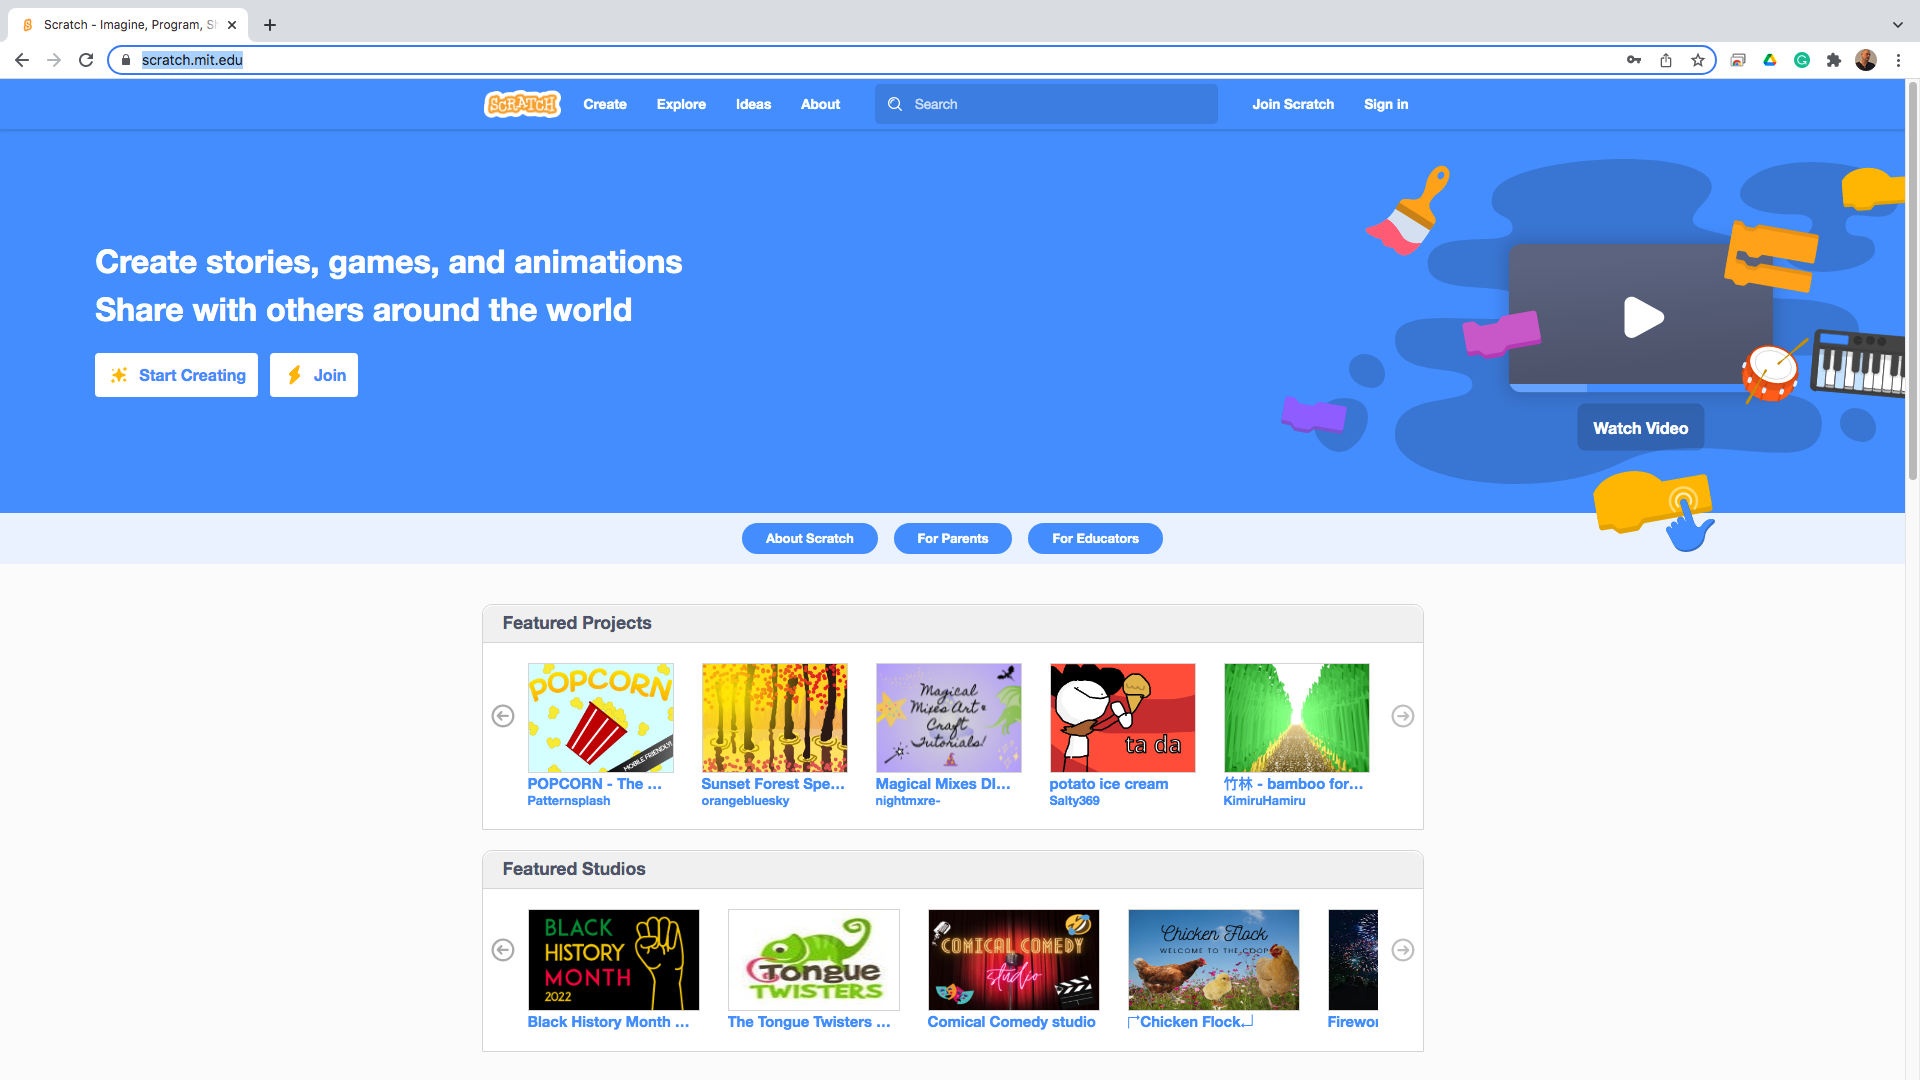
\includegraphics[width=1.0\linewidth,height=0.5\linewidth]{fig010001.png}
   \caption{Sratch Homepage}
\label{fig010001}
\end{figure}

The Scratch program environment operates based on cloud services. Therefore, individuals must register by creating an account to use the service. Registration entails providing a username and password (See Fig. \ref{fig010002} for a visual representation, which unfortunately cannot be displayed in a text-based conversation).

By registering, users gain access to the full functionality of Scratch, including the ability to save and share their projects, collaborate with others, and participate in the Scratch community.

\begin{figure}[H]
   \centering
   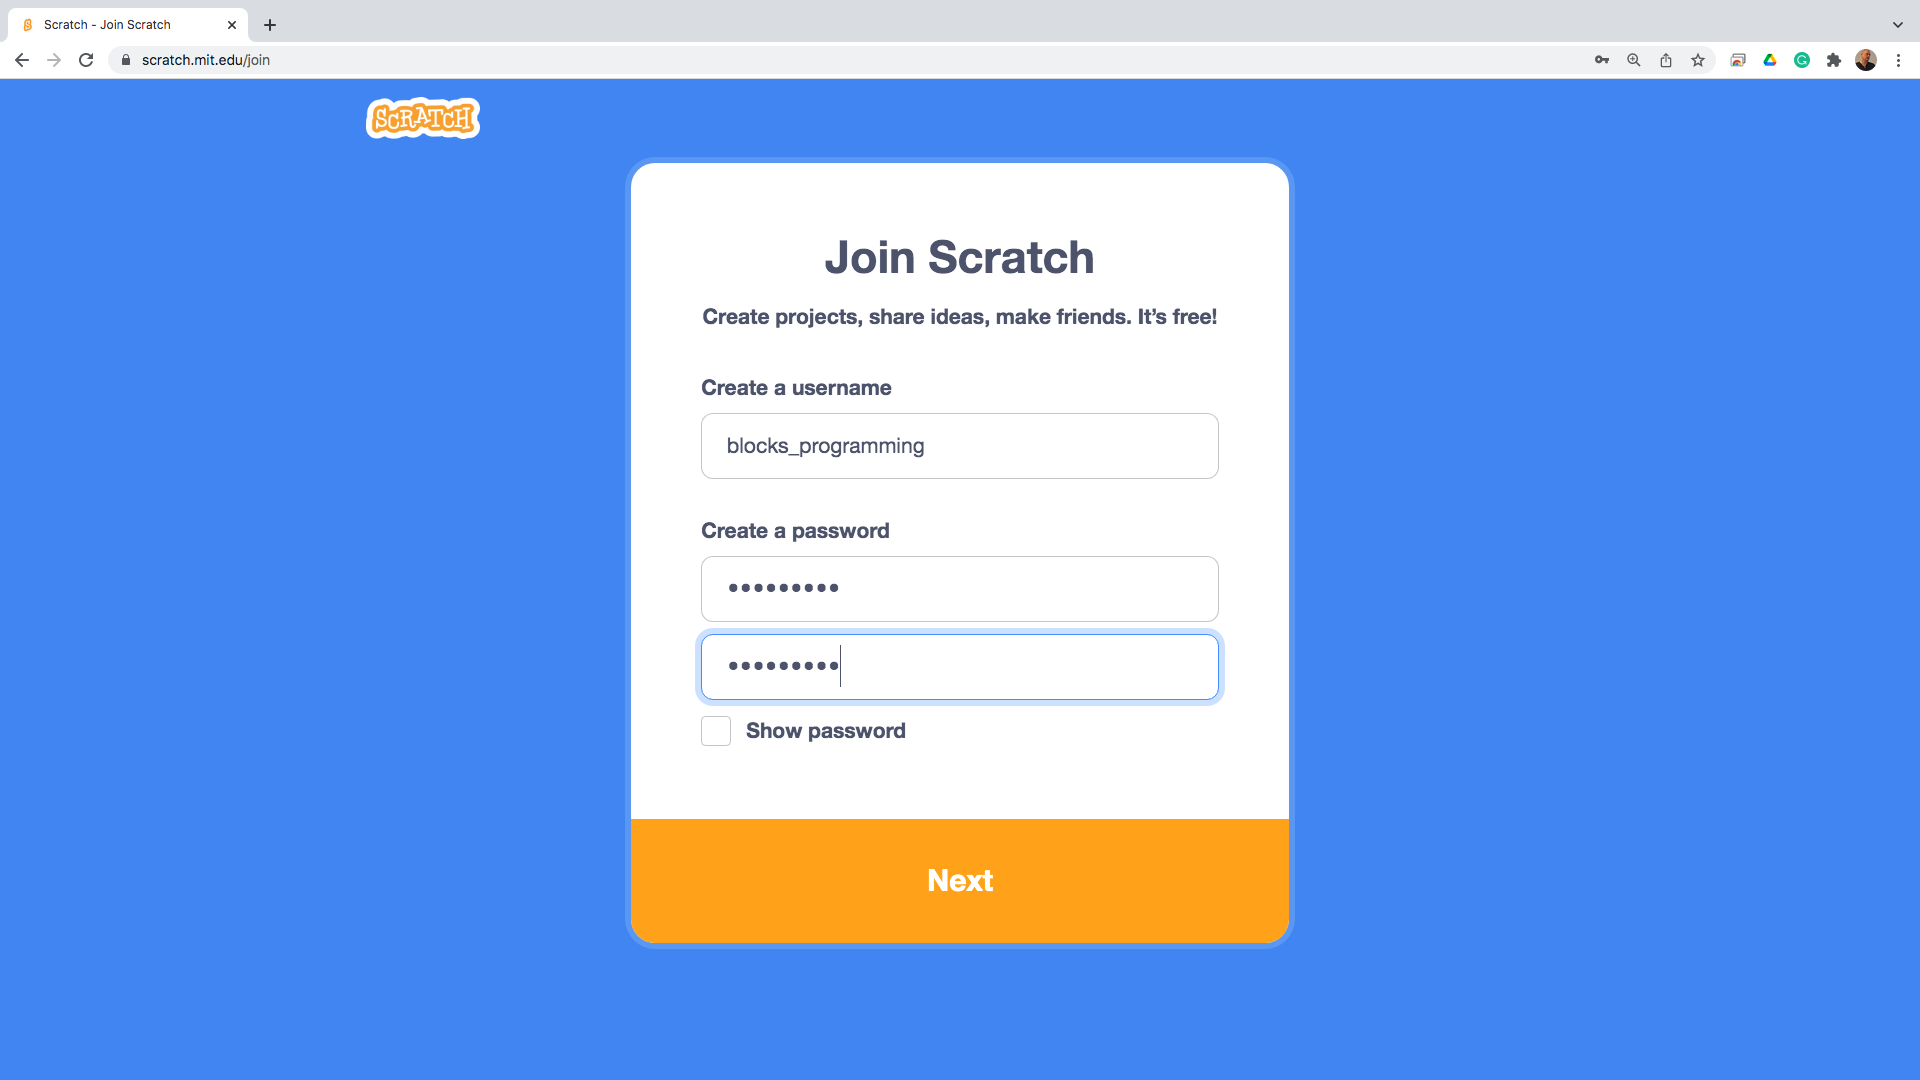
\includegraphics[width=1.0\linewidth,height=0.5\linewidth]{fig010002.png}
   \caption{Sratch User Registration}
\label{fig010002}
\end{figure}

After selecting a username and password during the registration process in Scratch (Fig. \ref{fig010002}), the next step typically involves specifying the geographical region where the user is located (Fig. \ref{fig010003}, which cannot be displayed in a text-based format). This information helps Scratch provide localized content, relevant events, and community engagement opportunities that may be specific to the user's region.

Users can further personalize their Scratch experience by selecting the geographical region and connecting with other Scratch users from their area.

\begin{figure}[H]
   \centering
   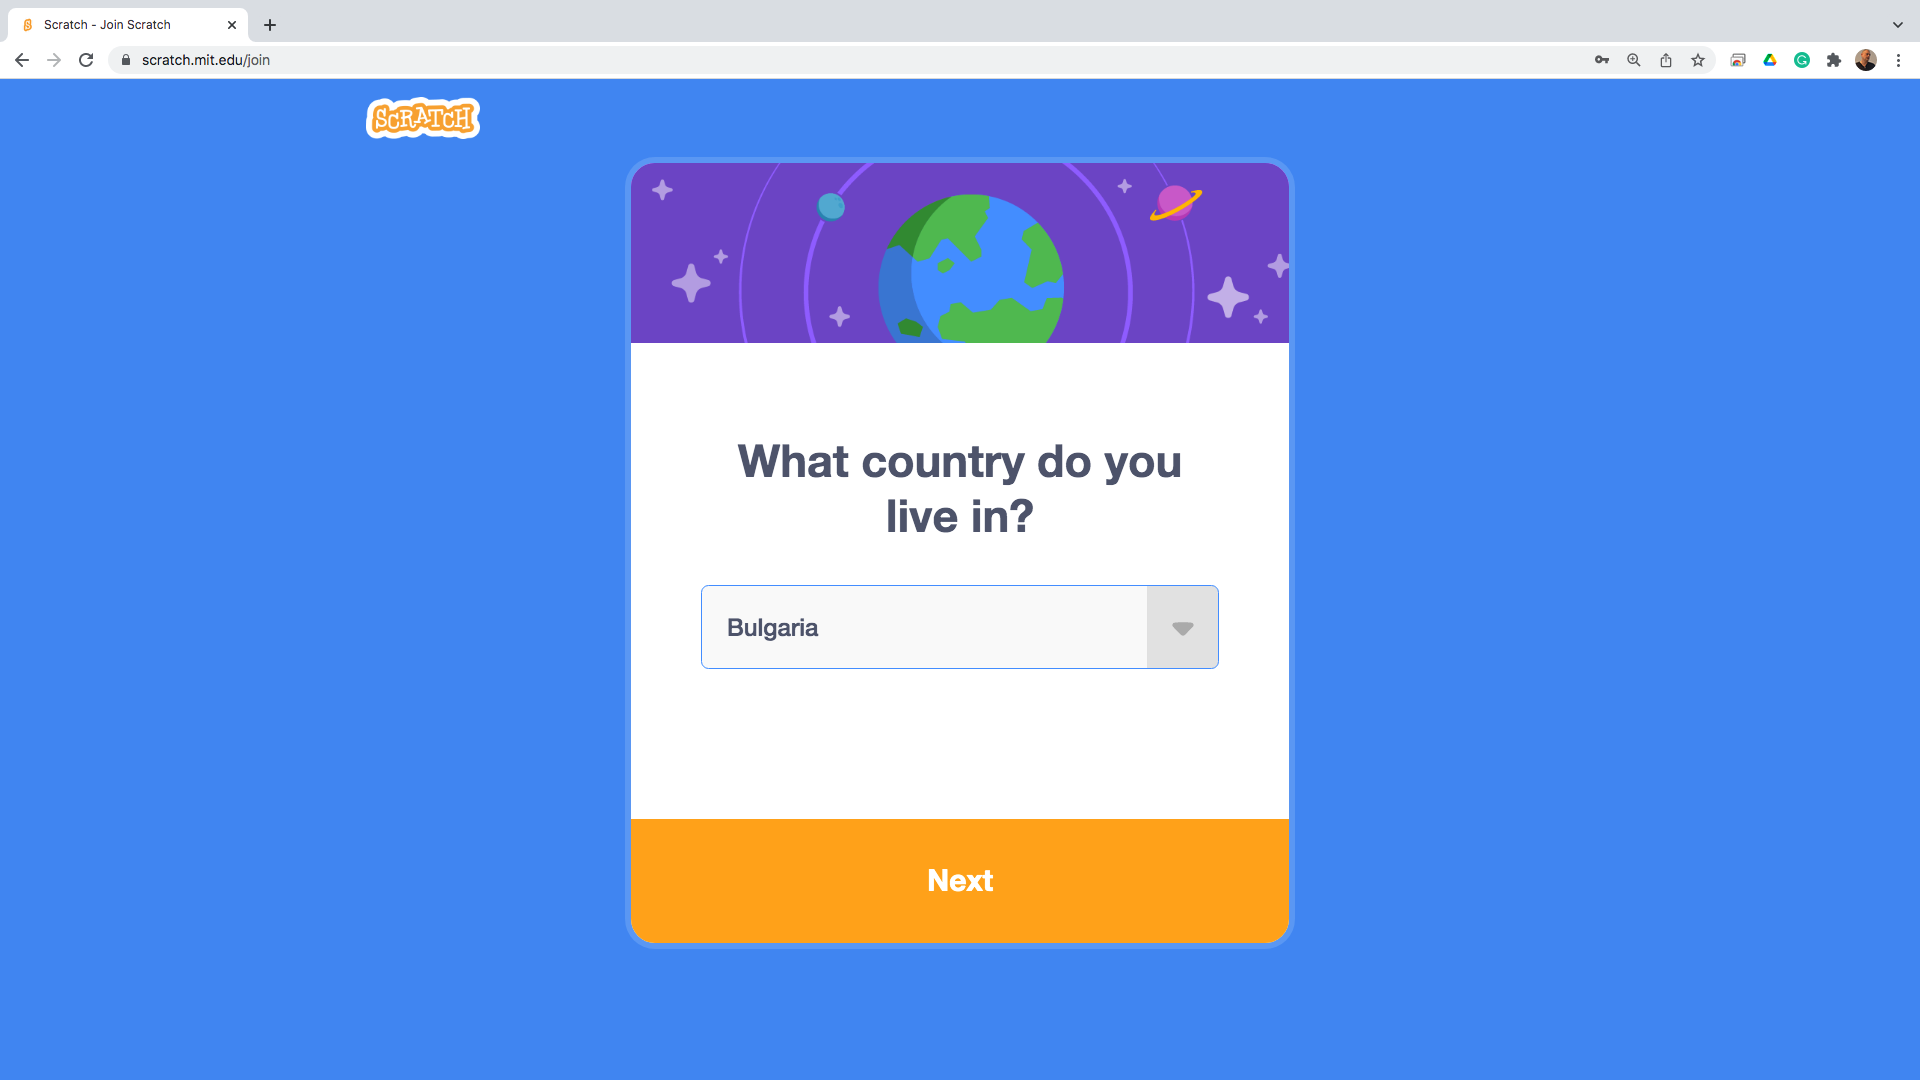
\includegraphics[width=1.0\linewidth,height=0.5\linewidth]{fig010003.png}
   \caption{Geographic location}
\label{fig010003}
\end{figure}

The Scratch platform is primarily designed for children who are interested in programming, as well as for parents and teachers. The system collects information about their age to cater to its user's specific needs and safety considerations (Fig. \ref{fig010004}, which cannot be displayed in a text-based format). By gathering age information, Scratch can provide age-appropriate content, features, and interactions suitable for the specific user group.

This age information helps tailor the experience within Scratch, ensuring that the platform offers appropriate educational resources and maintains a safe and supportive environment for young users. It also enables parents and teachers to guide and supervise children's activities on the platform effectively.

\begin{figure}[H]
   \centering
   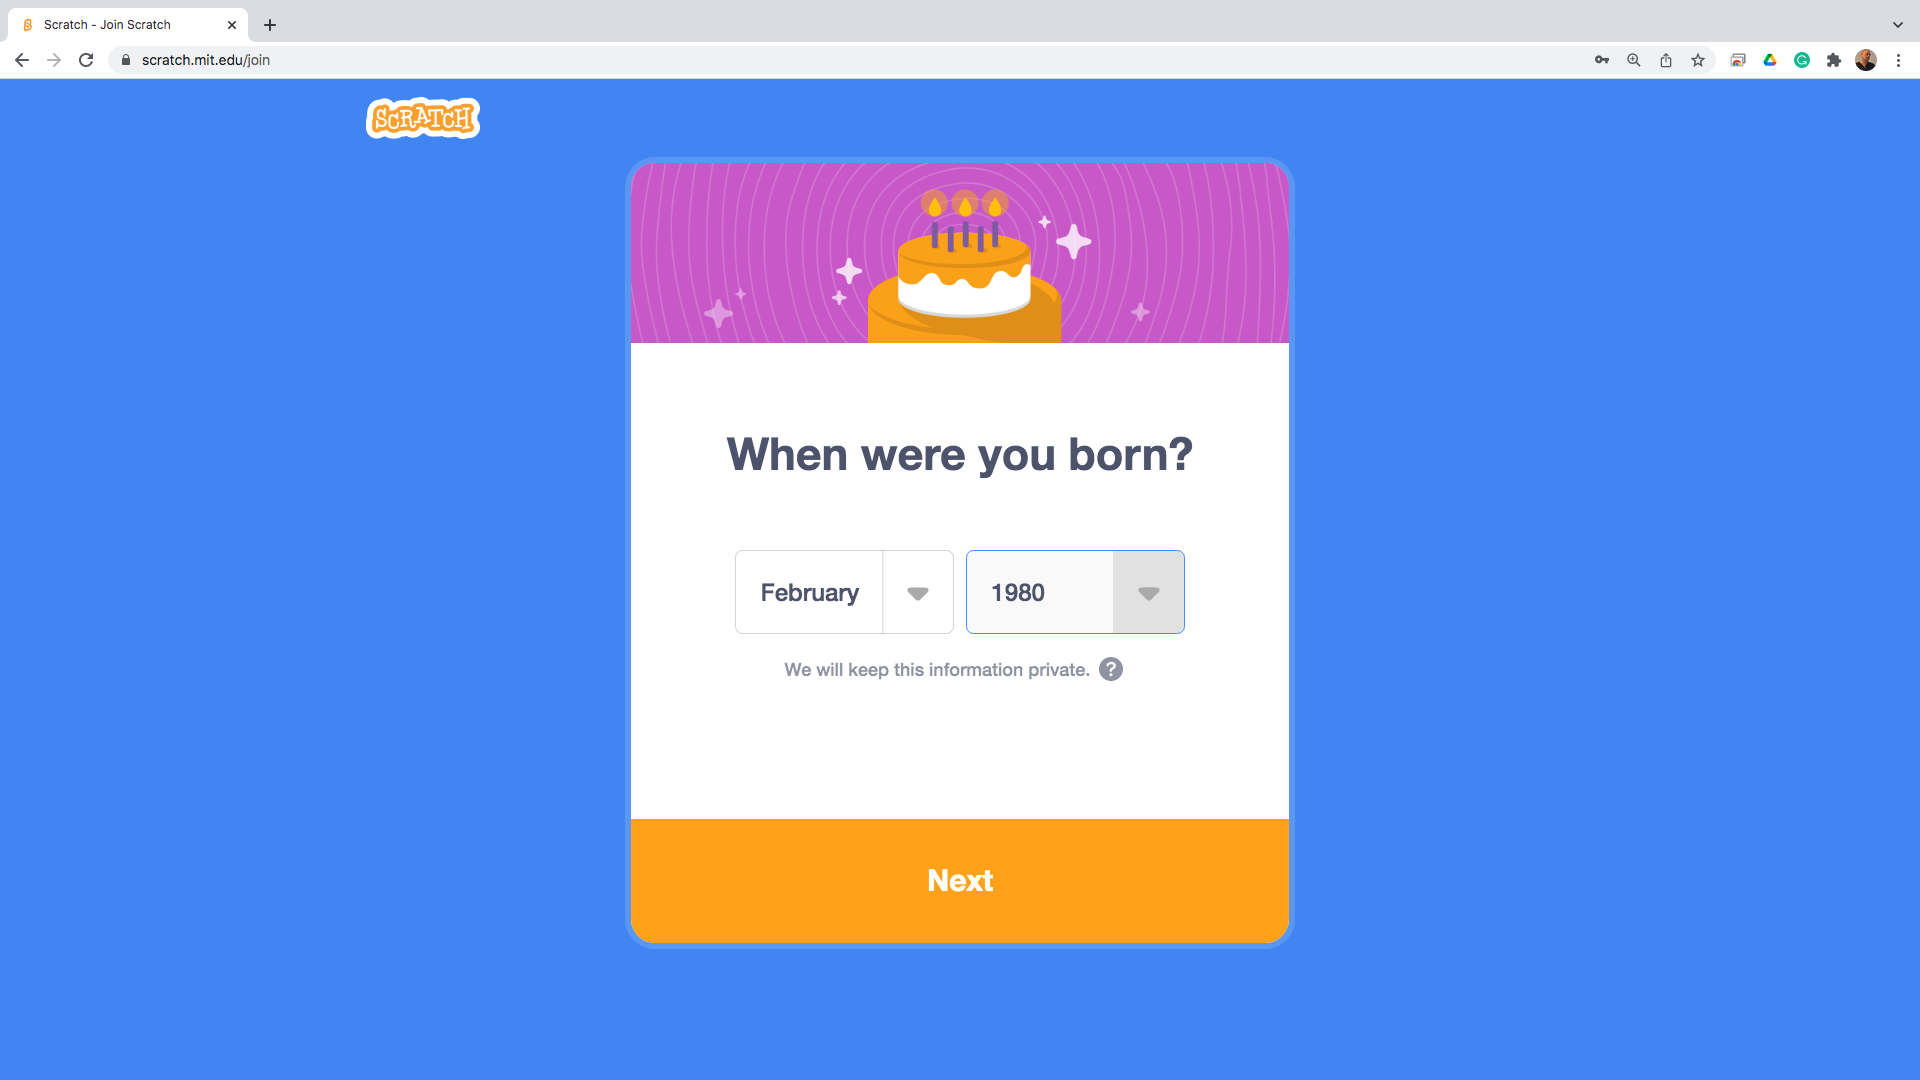
\includegraphics[width=1.0\linewidth,height=0.5\linewidth]{fig010004.png}
   \caption{Age of User}
\label{fig010004}
\end{figure}

In addition to collecting information about the user's age, the Scratch system also offers the option to provide information regarding gender classification (Fig. \ref{fig010005}, which unfortunately cannot be displayed in a text-based conversation). However, it's important to note that providing gender information is optional, and users can choose not to disclose it if they prefer.

The inclusion of gender classification is primarily aimed at fostering an inclusive and diverse community within Scratch. It allows for tailored content and experiences that address various interests and perspectives. By making this information optional, Scratch aims to prevent any form of discrimination based on gender while respecting the privacy and preferences of its users.

\begin{figure}[H]
   \centering
   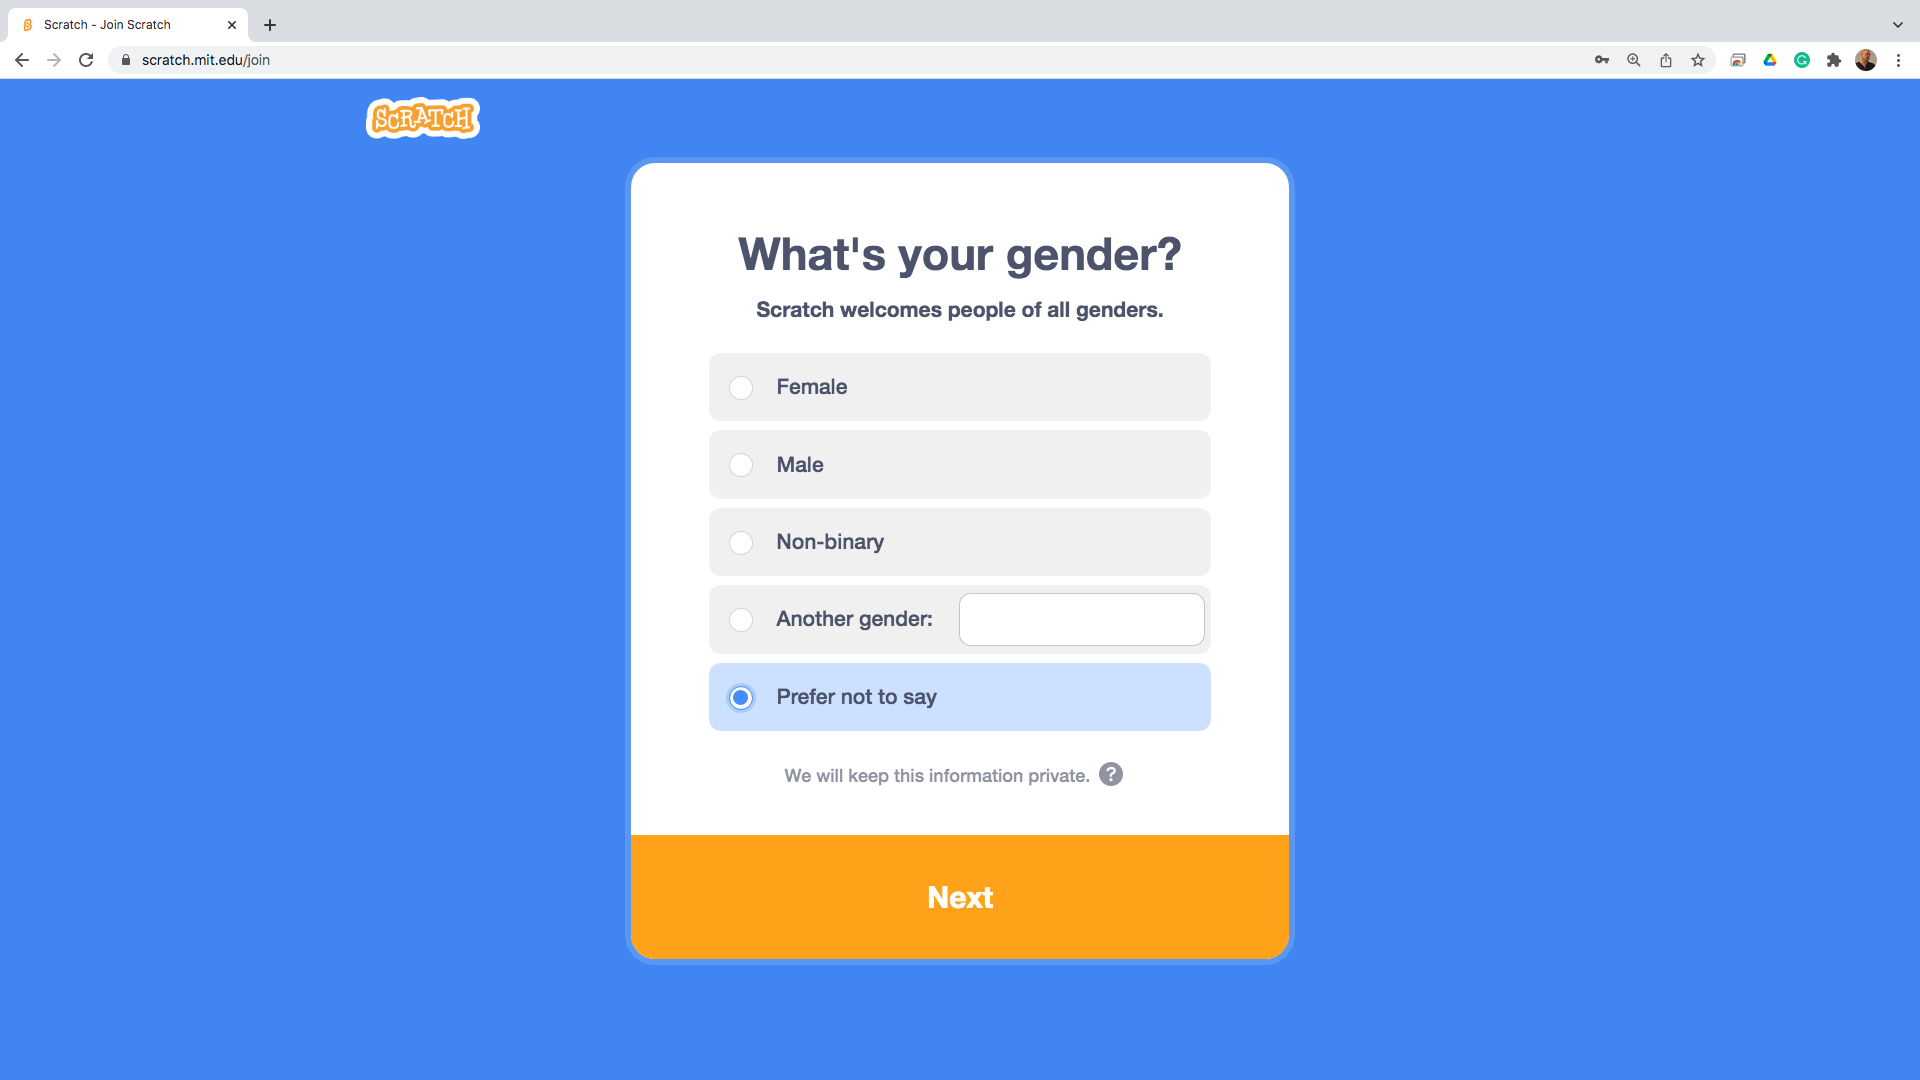
\includegraphics[width=1.0\linewidth,height=0.5\linewidth]{fig010005.png}
   \caption{User gender}
\label{fig010005}
\end{figure}

To create a user profile on Scratch, along with selecting a username and password, it is required to associate the profile with an email address (Fig. \ref{fig010006}, which cannot be displayed in a text-based format). The email address serves as a means of communication and verification for the user account.

Users can receive important notifications, account-related updates, and password reset instructions if necessary by providing an email address. It also helps maintain the security and integrity of the user's profile. The email address is treated with confidentiality and is not publicly visible to other Scratch users.

\begin{figure}[H]
   \centering
   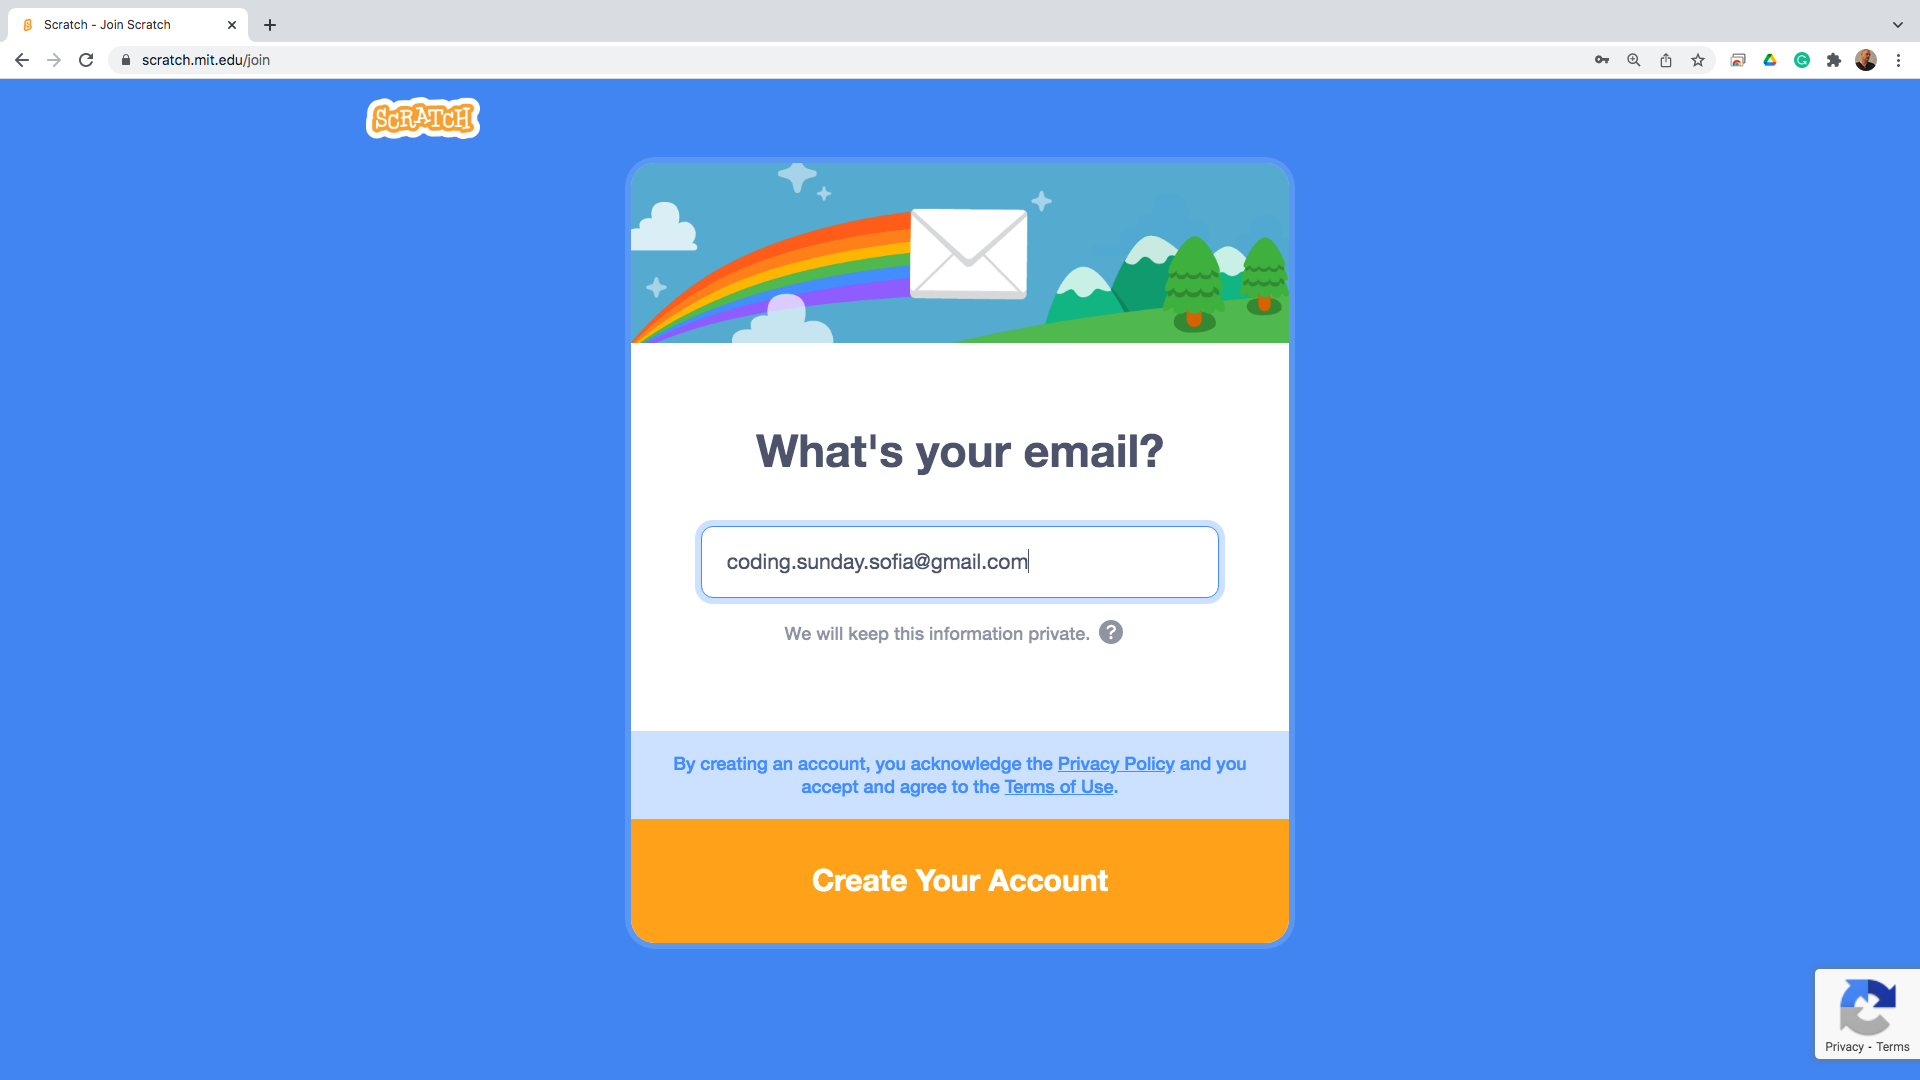
\includegraphics[width=1.0\linewidth,height=0.5\linewidth]{fig010006.png}
   \caption{User email address}
\label{fig010006}
\end{figure}

Once the user registration process in the system is nearly complete (Fig. \ref{fig010007}, which cannot be displayed in a text-based format), the final step is to confirm the selected email address. This step ensures the provided email's accuracy and helps verify the user's identity.

After entering the email address during registration, Scratch sends a confirmation email to the provided address. The user must then access their email inbox, find the verification email from Scratch, and follow the instructions to confirm the email address. This step helps prevent unauthorized access and ensures the user has control over the associated email account.

By confirming the email address, users can fully activate their Scratch account and gain access to all the features and benefits offered by the platform.

\begin{figure}[H]
   \centering
   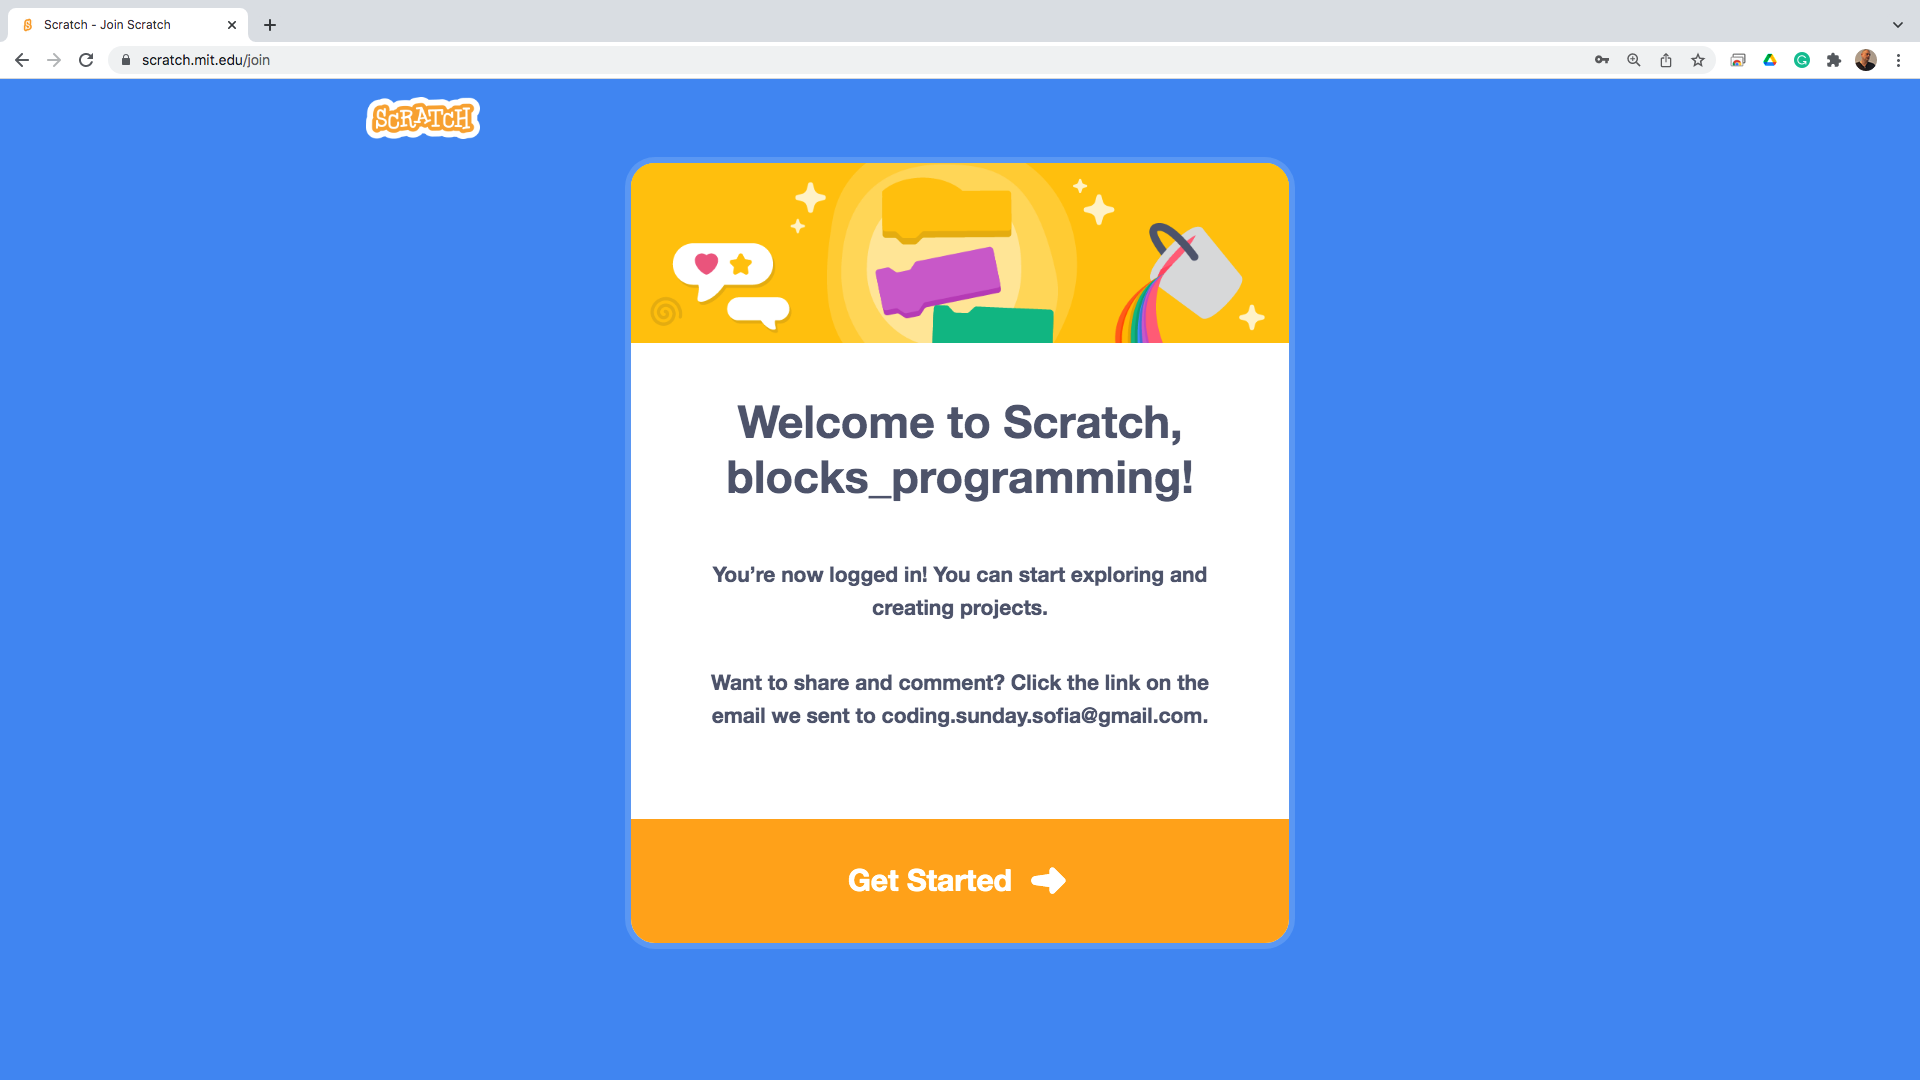
\includegraphics[width=1.0\linewidth,height=0.5\linewidth]{fig010007.png}
   \caption{Completing the user information entry process}
\label{fig010007}
\end{figure}

When a user registers in Scratch and reaches the stage of email confirmation, they will receive an email that includes an electronic link to the Scratch website (Fig. \ref{fig010008}, which unfortunately cannot be displayed in a text-based format). This link must be clicked or followed to finalize the new user registration process.

The user will be directed to a specific page on the Scratch website by clicking on the link provided in the email. This page typically confirms that the user's email address has been successfully verified, completing the registration process.

Following the link is crucial to validate the email address and ensure the user's account activation. It is an essential step to provide a secure and legitimate registration process within the Scratch platform.

\begin{figure}[H]
   \centering
   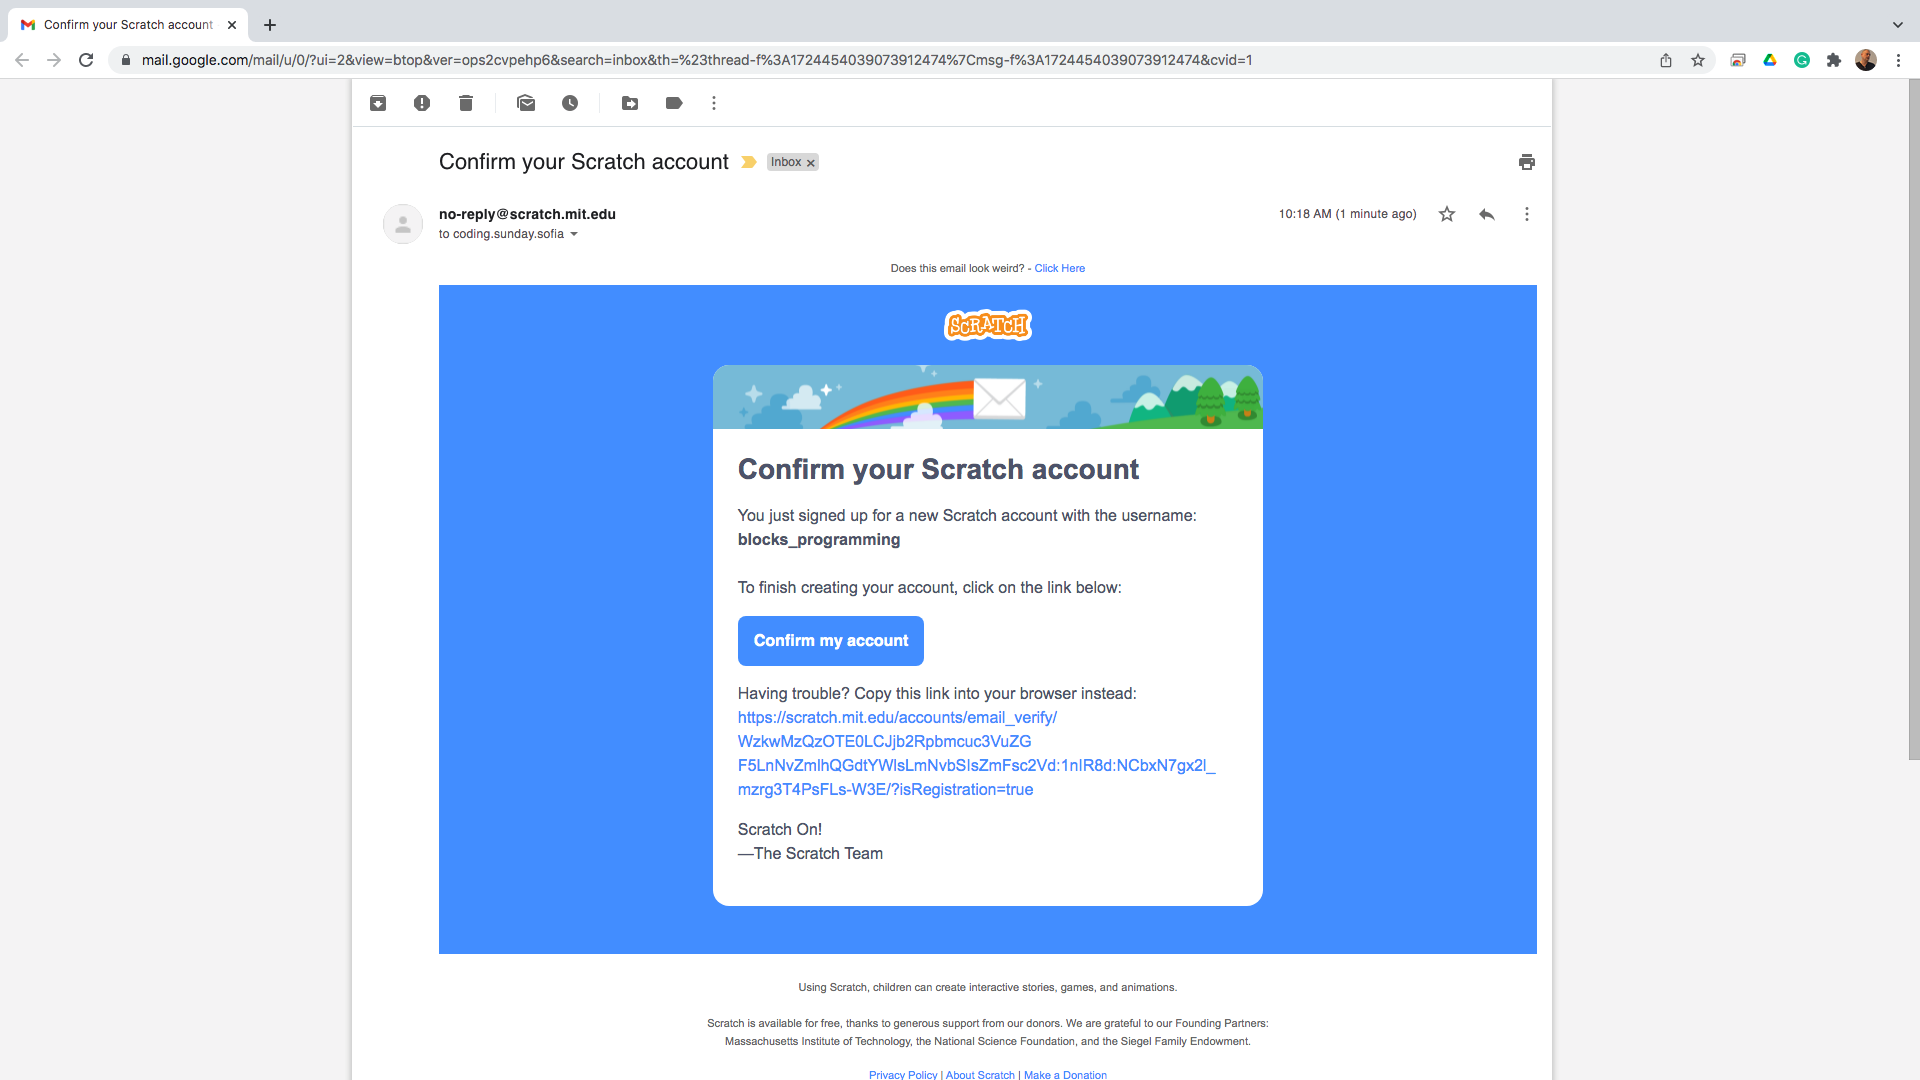
\includegraphics[width=1.0\linewidth,height=0.5\linewidth]{fig010008.png}
   \caption{Email confirmation email}
\label{fig010008}
\end{figure}

The registration process for a new user concludes with loading the initial working screen in Scratch (Fig. \ref{fig010009}, which cannot be displayed in a text-based format). At the top right corner of the screen, you will find the username chosen during the first step of the registration process.

Upon reaching the working screen, users can start exploring and utilizing Scratch's various features and tools to create their interactive projects. The username displayed at the top right corner is a quick reference to identify the logged-in user and allows easy access to their account settings and project management options.

\begin{figure}[H]
   \centering
   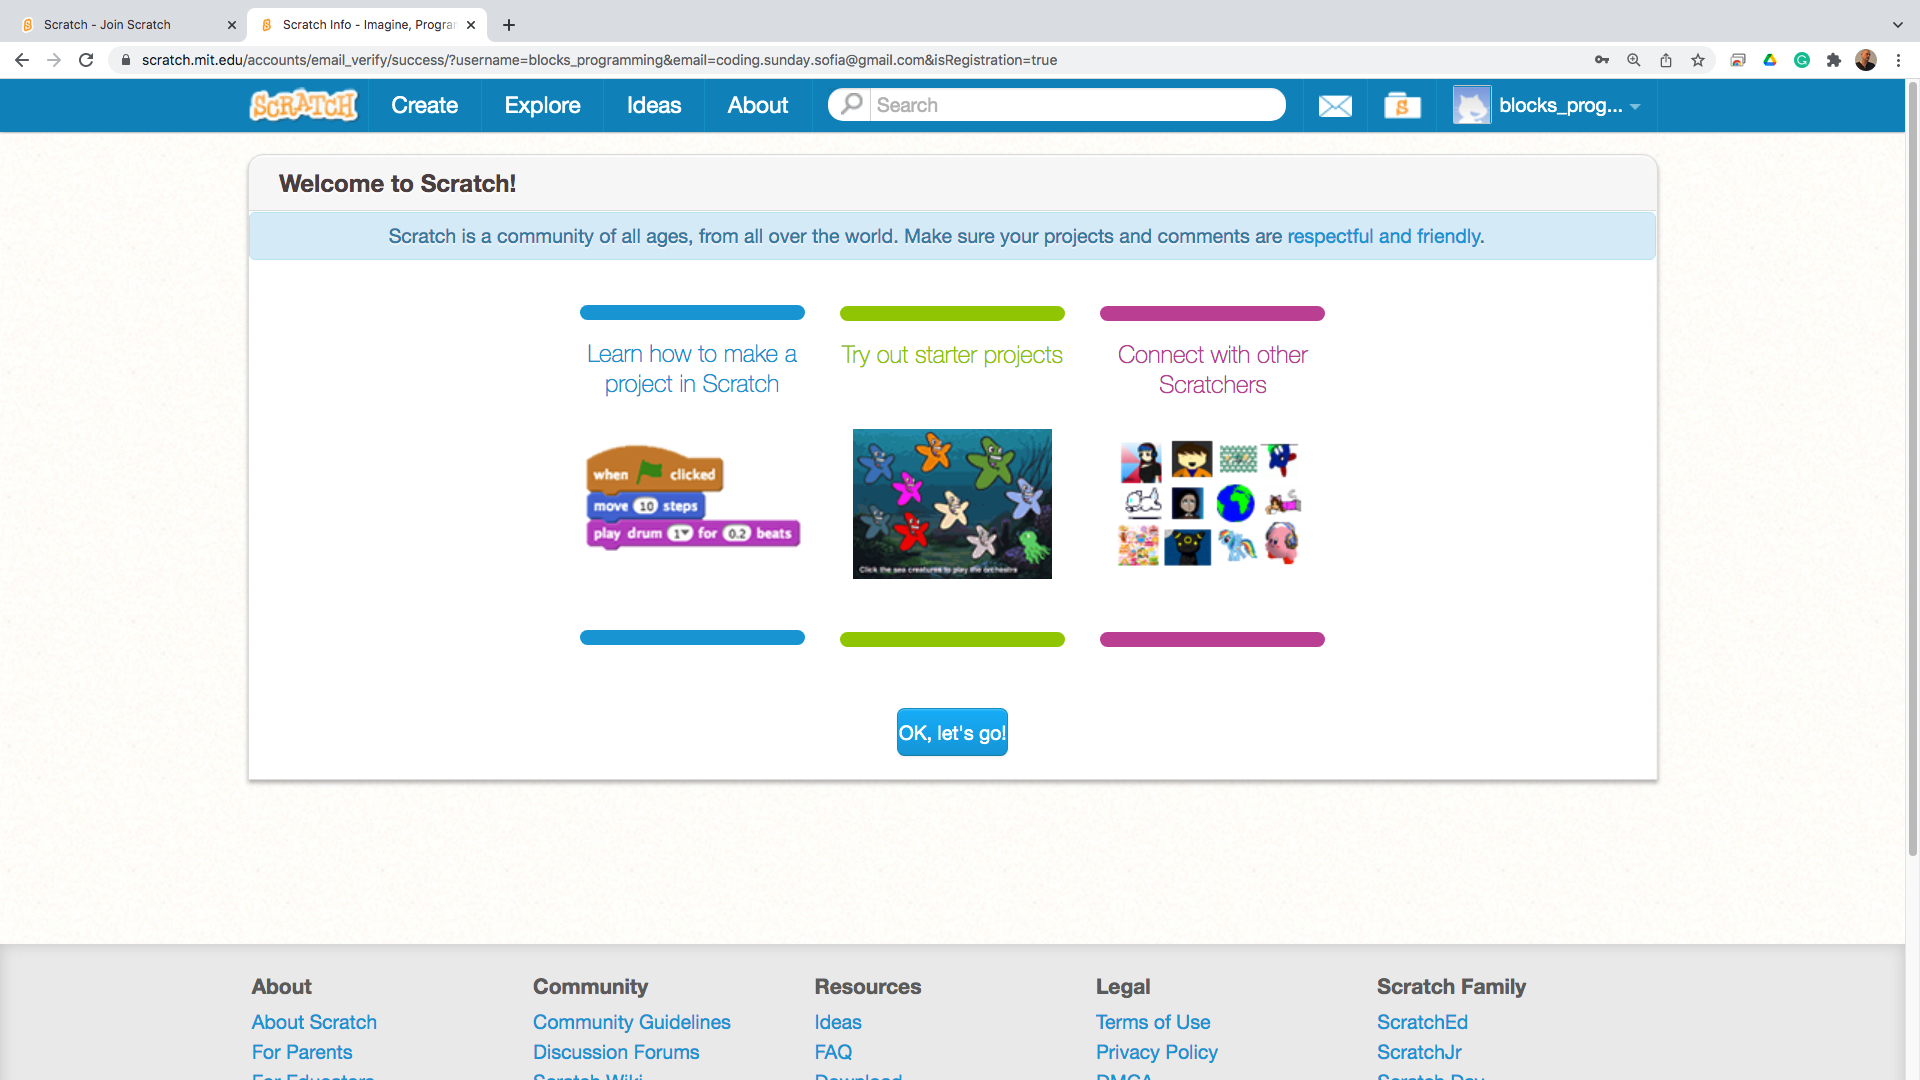
\includegraphics[width=1.0\linewidth,height=0.5\linewidth]{fig010009.png}
   \caption{Home screen}
\label{fig010009}
\end{figure}

To confirm a successful registration in Scratch, users can create a small project to experience the development environment in action. This can be done by selecting the "Create" option from the menu (Fig. \ref{fig010010}, which cannot be displayed in a text-based conversation).

By choosing the "Create" option, users will be directed to the project editor to build their own interactive projects using blocks and scripts. This demonstrates that the registration process was completed successfully and that users now have access to the full functionality of Scratch.

Creating a small project not only allows users to familiarize themselves with the development environment but also serves as a practical demonstration of their ability to utilize Scratch's features and begin exploring the possibilities of programming and coding within the platform.

\begin{figure}[H]
   \centering
   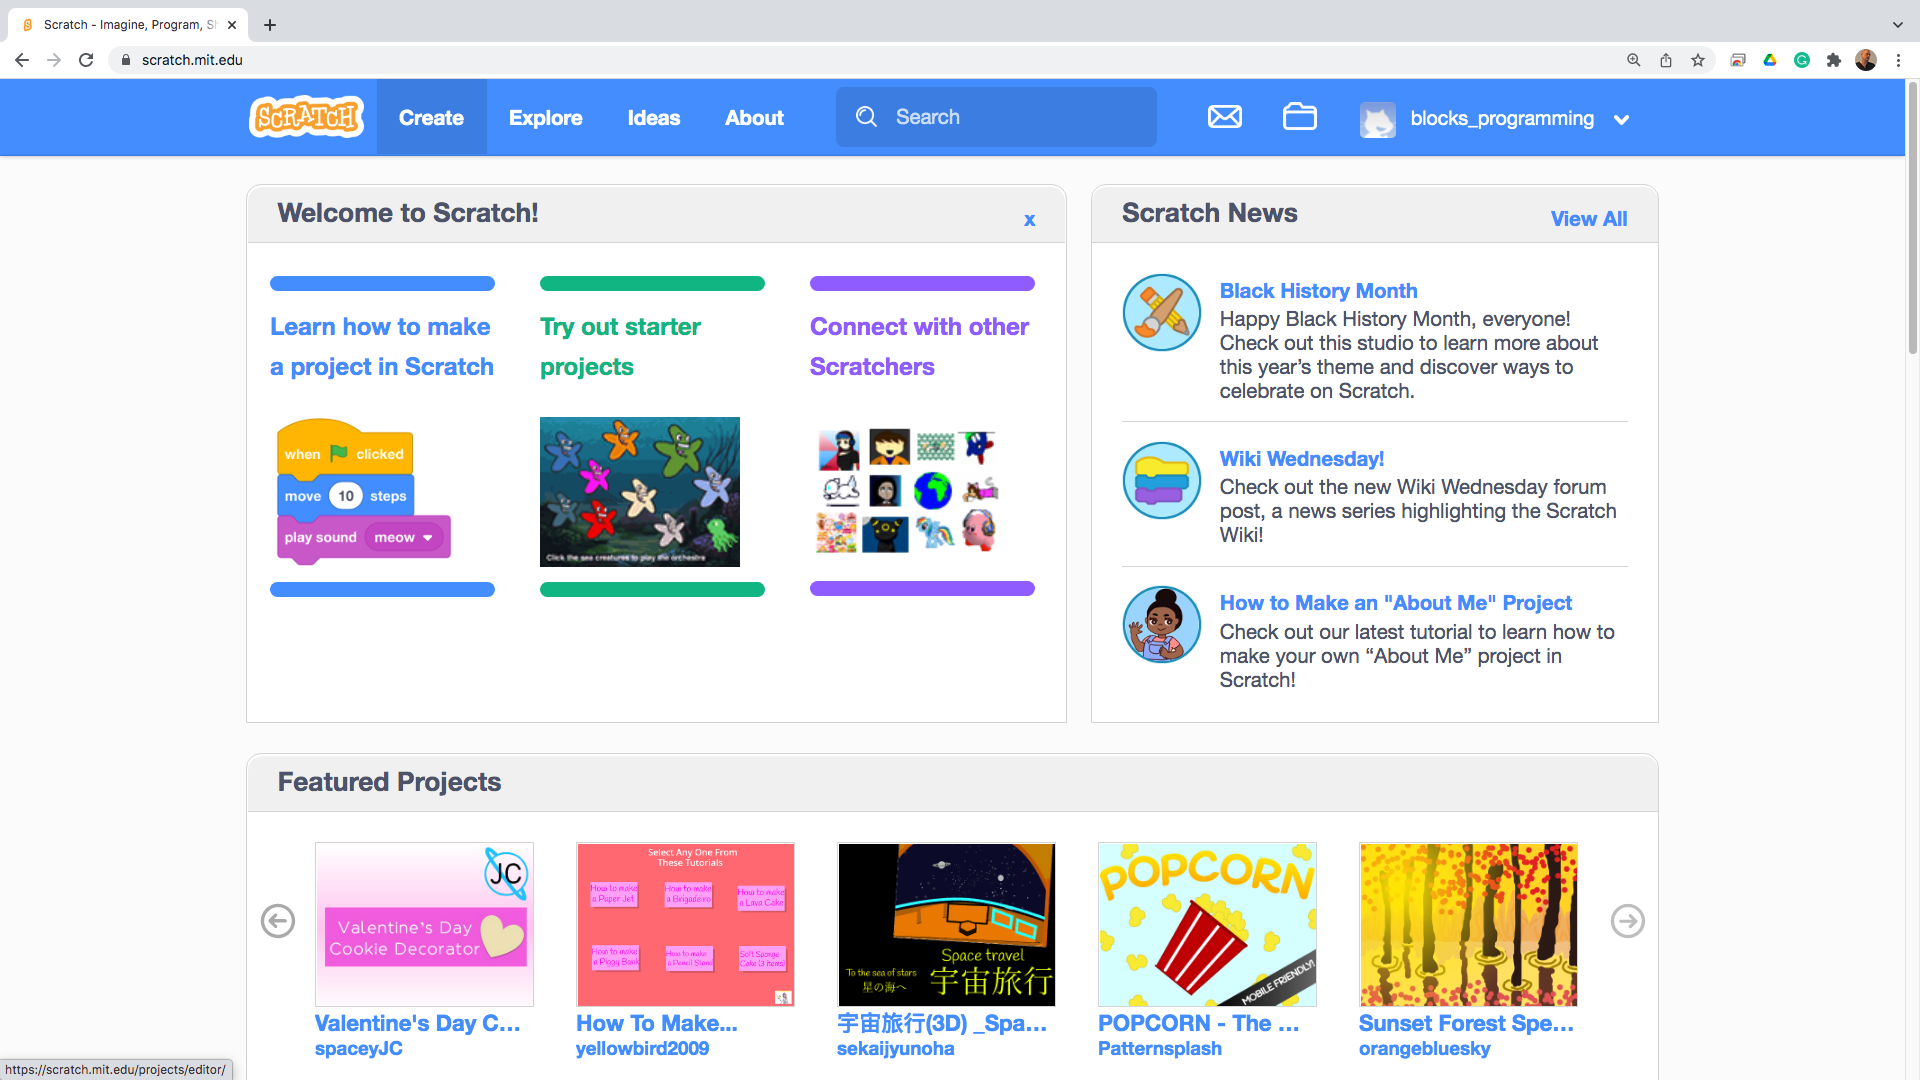
\includegraphics[width=1.0\linewidth,height=0.5\linewidth]{fig010010.png}
   \caption{Selecting a New Project Menu Option}
\label{fig010010}
\end{figure}

When creating a new project in Scratch, the process involves several steps related to allocating the initially required resources (Fig. \ref{fig010011}, which cannot be displayed in a text-based format). These steps ensure that users have the necessary components to build their projects.

Typically, the resource allocation steps include selecting a backdrop (the background image or scene for the project), choosing sprites (the characters or objects that will interact in the project), and possibly importing additional media files such as sounds or images.

By going through these steps, users can set up the initial elements of their project, providing a foundation for further development and programming. It allows users to define their project's visual and auditory aspects before moving on to coding and creating interactions between the sprites and backdrop.

\begin{figure}[H]
   \centering
   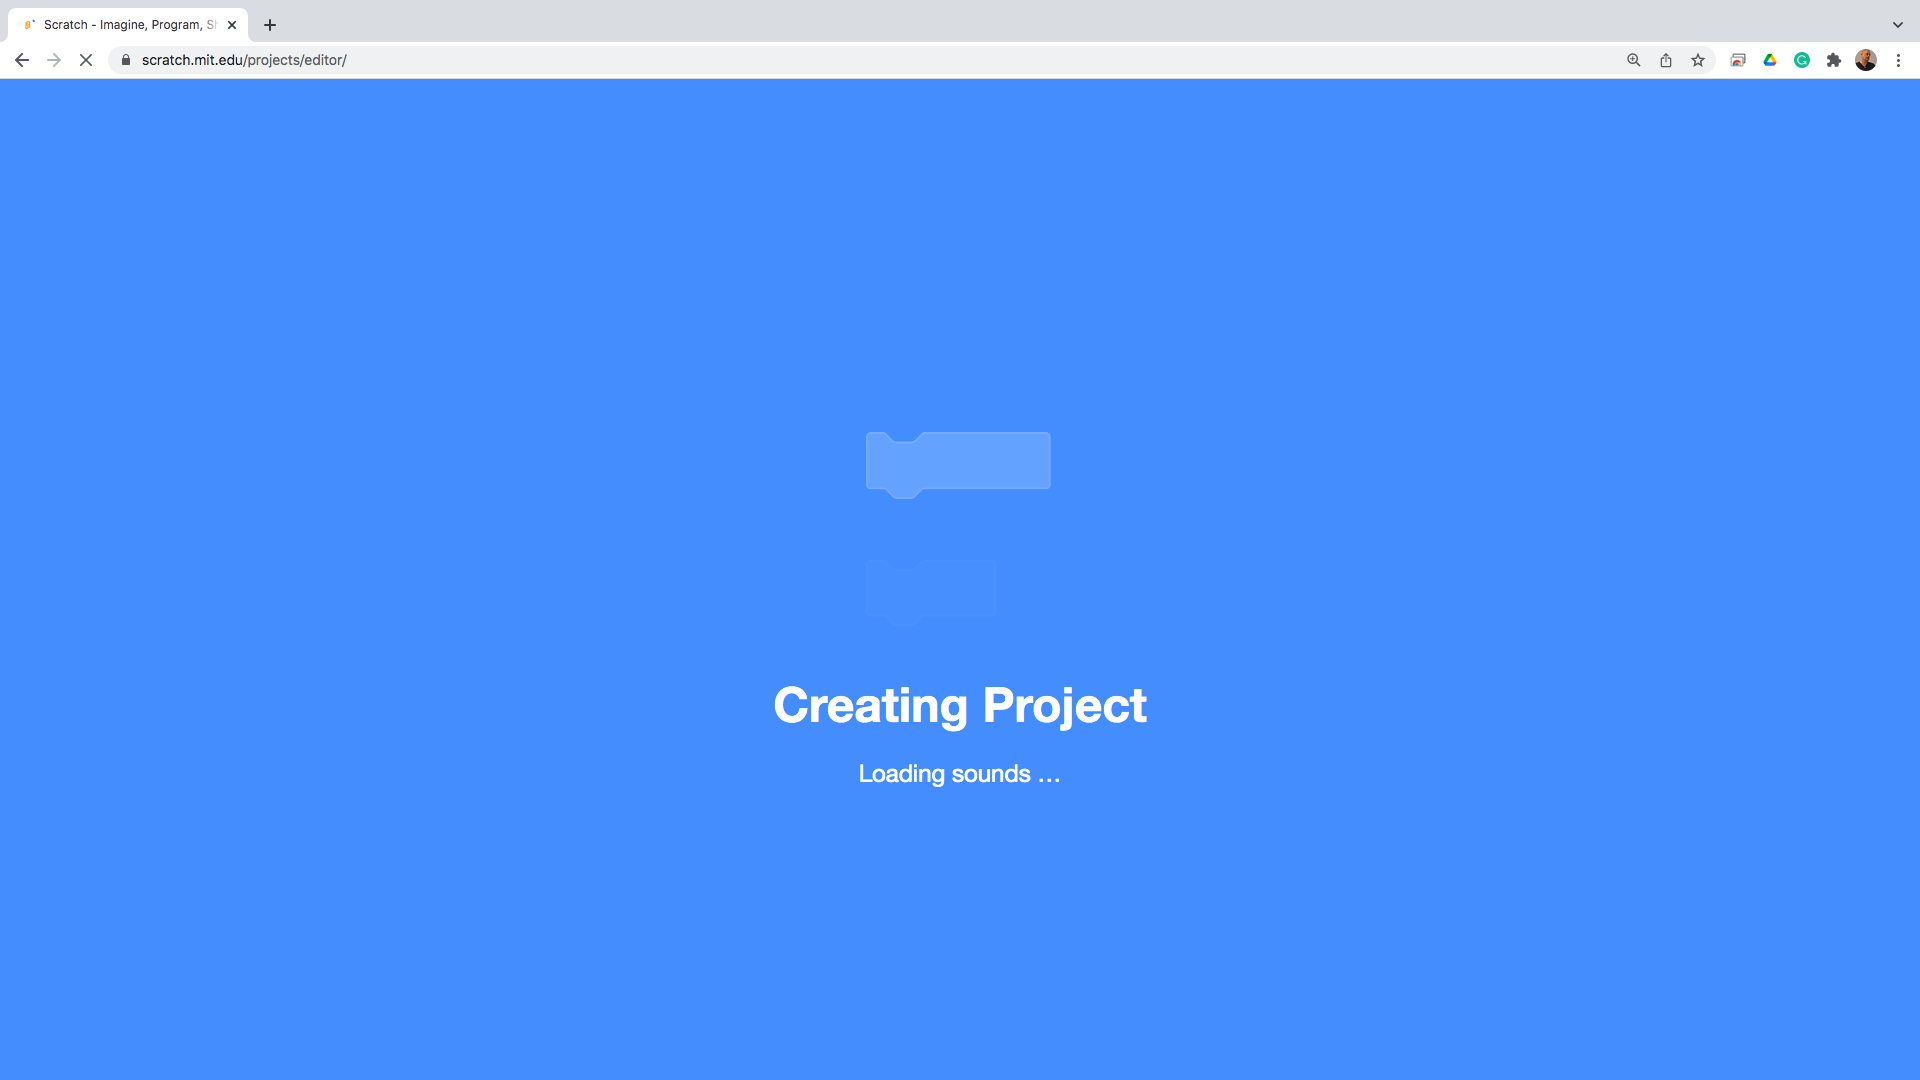
\includegraphics[width=1.0\linewidth,height=0.5\linewidth]{fig010011.png}
   \caption{Loading Resources}
\label{fig010011}
\end{figure}

Once the new project is loaded, users will be presented with the workspace in Scratch (Fig. \ref{fig010012}, which cannot be displayed in a text-based format). The workspace is divided into three main sections:

1. the list of available program instructions is on the far left, represented as puzzle pieces. These blocks contain different commands and functions that users can drag and drop into the workspace to build their program.

2. In the central part of the workspace is where users arrange and connect the program instructions. They can snap together the blocks to create a sequence of actions and define the logic of their project.

3. On the far right is the active stage, where the visual representation of the project is displayed. It shows the results of the actions embedded in the series of instructions as users interact with and run their program.

This workspace layout allows users to visually construct their program by assembling the puzzle-like blocks, creating a clear and intuitive interface for programming and coding within Scratch.

\begin{figure}[H]
   \centering
   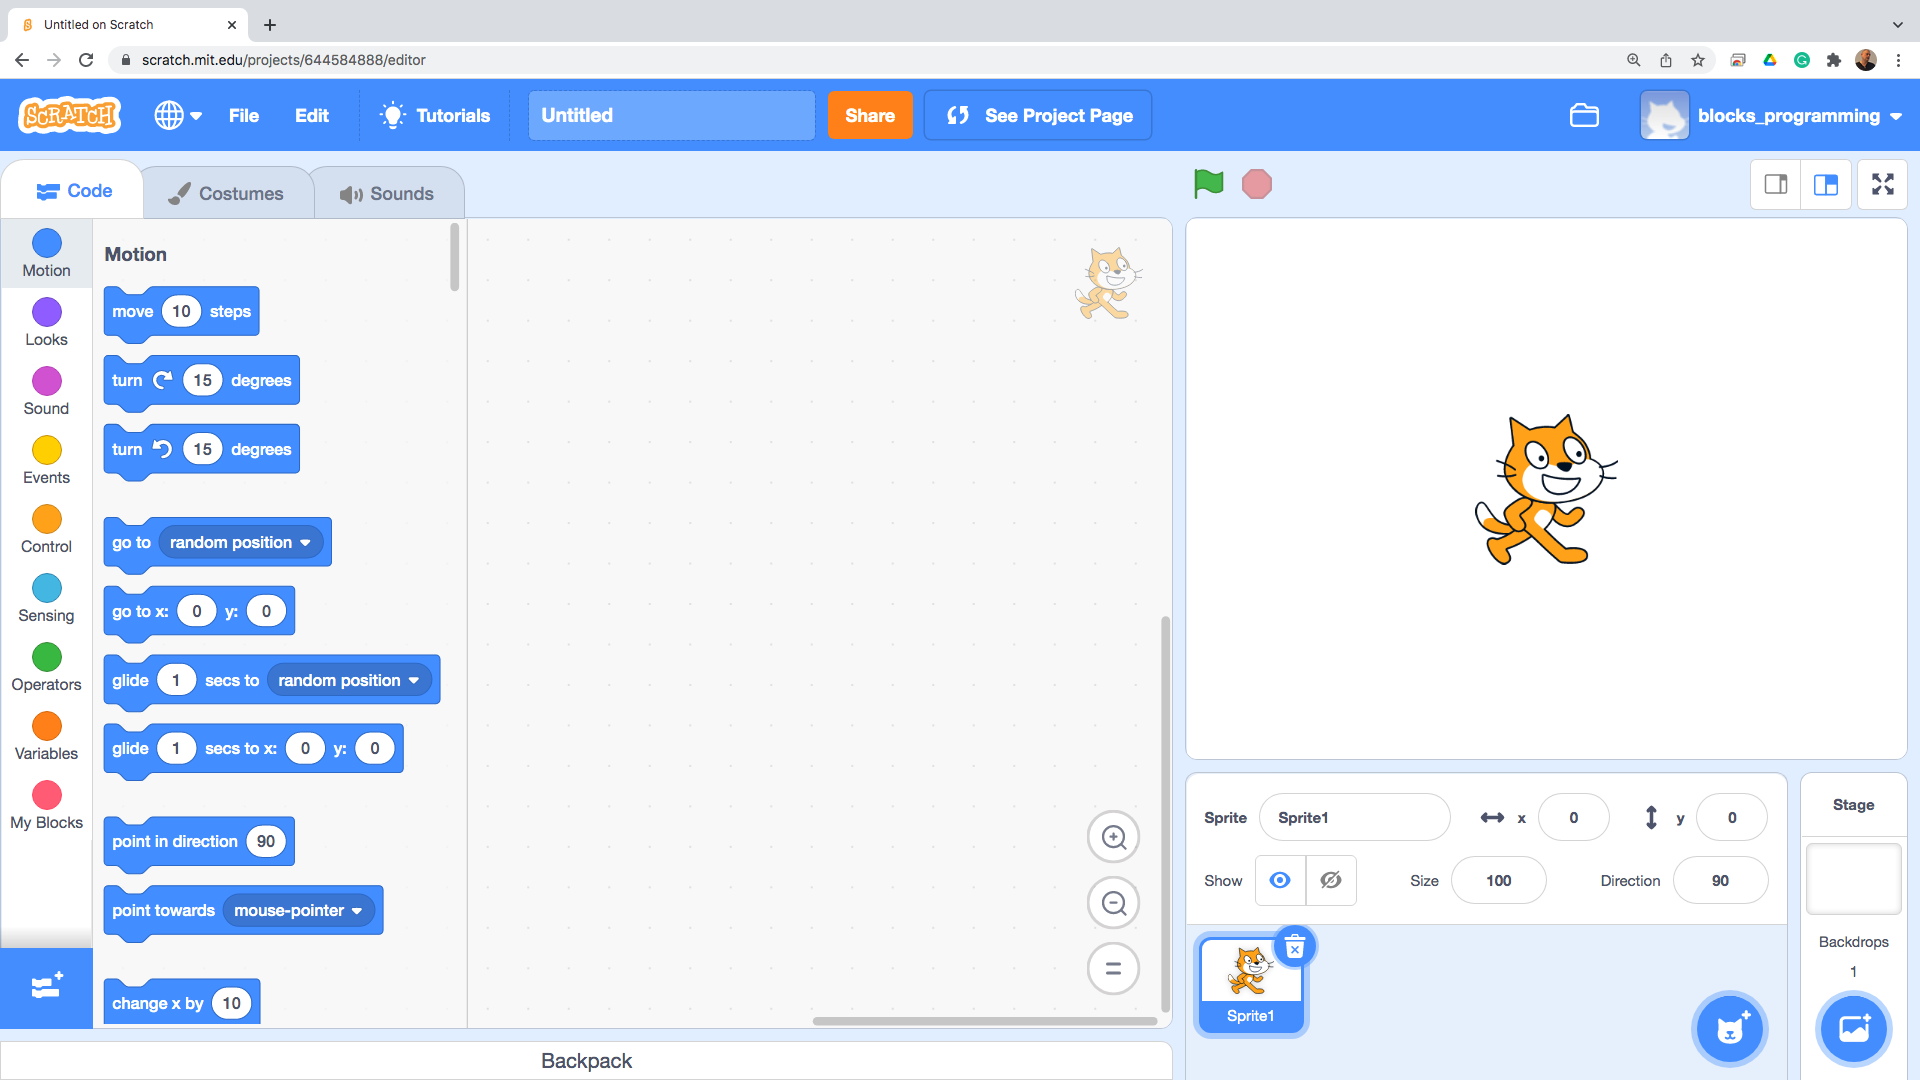
\includegraphics[width=1.0\linewidth,height=0.5\linewidth]{fig010012.png}
   \caption{Workspace Organization}
\label{fig010012}
\end{figure}

In Scratch, every computer program has designated starting and ending points. To signify the beginning of a program, Scratch provides a particular block known as the program launch block (Fig. \ref{fig010013}, which cannot be displayed in a text-based format).

The program launch block is tied explicitly to the green flag click event. When the green flag is clicked in the Scratch environment, the program execution begins. This block serves as a trigger, indicating that the program should start running and that the actions and instructions defined in the blocks connected to it will be executed.

By associating the program launch block with the green flag click event, Scratch ensures a clear and consistent way to initiate the execution of programs, allowing users to interact with their projects and observe the desired behavior or animations when the green flag is clicked.

\begin{figure}[H]
   \centering
   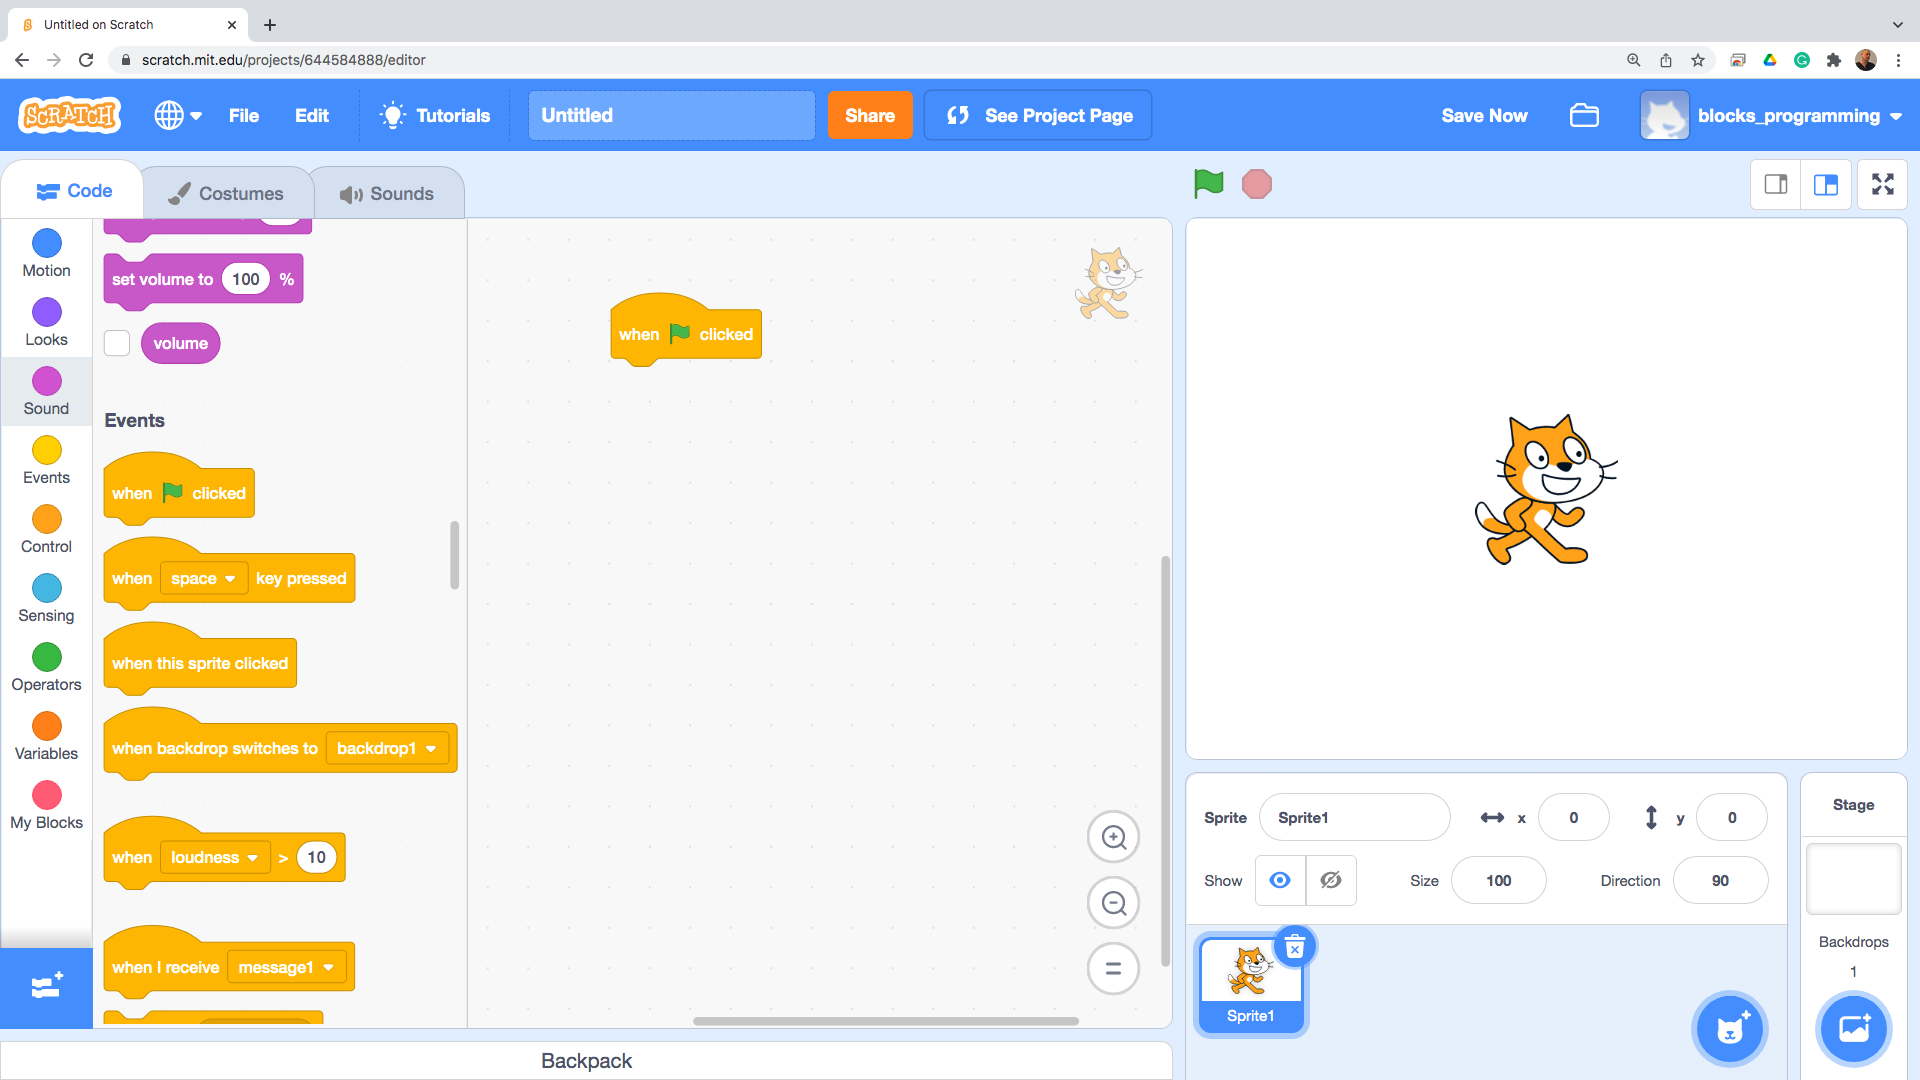
\includegraphics[width=1.0\linewidth,height=0.5\linewidth]{fig010013.png}
   \caption{Start of program}
\label{fig010013}
\end{figure}

One of Scratch's most uncomplicated and most intuitive instructions is the ability to move a sprite by a specified number of steps (Fig. \ref{fig010014}, which cannot be displayed in a text-based format). In the default opening scene of Scratch, the leading actor is the orange cat sprite. If the scene remains unchanged, the instructions to perform various actions will be applied directly to that cat sprite.

By using the "move" block and specifying the number of steps, users can control the sprite's movement within the Scratch stage. This instruction allows the sprite to move horizontally, vertically, or diagonally across the screen.

When creating a project, users can apply various actions and instructions to the orange cat sprite, such as moving, changing costumes, playing sounds, or interacting with other sprites or user inputs. This enables them to bring their ideas to life and create interactive stories, animations, and games using the familiar orange cat as the protagonist or main character.

\begin{figure}[H]
   \centering
   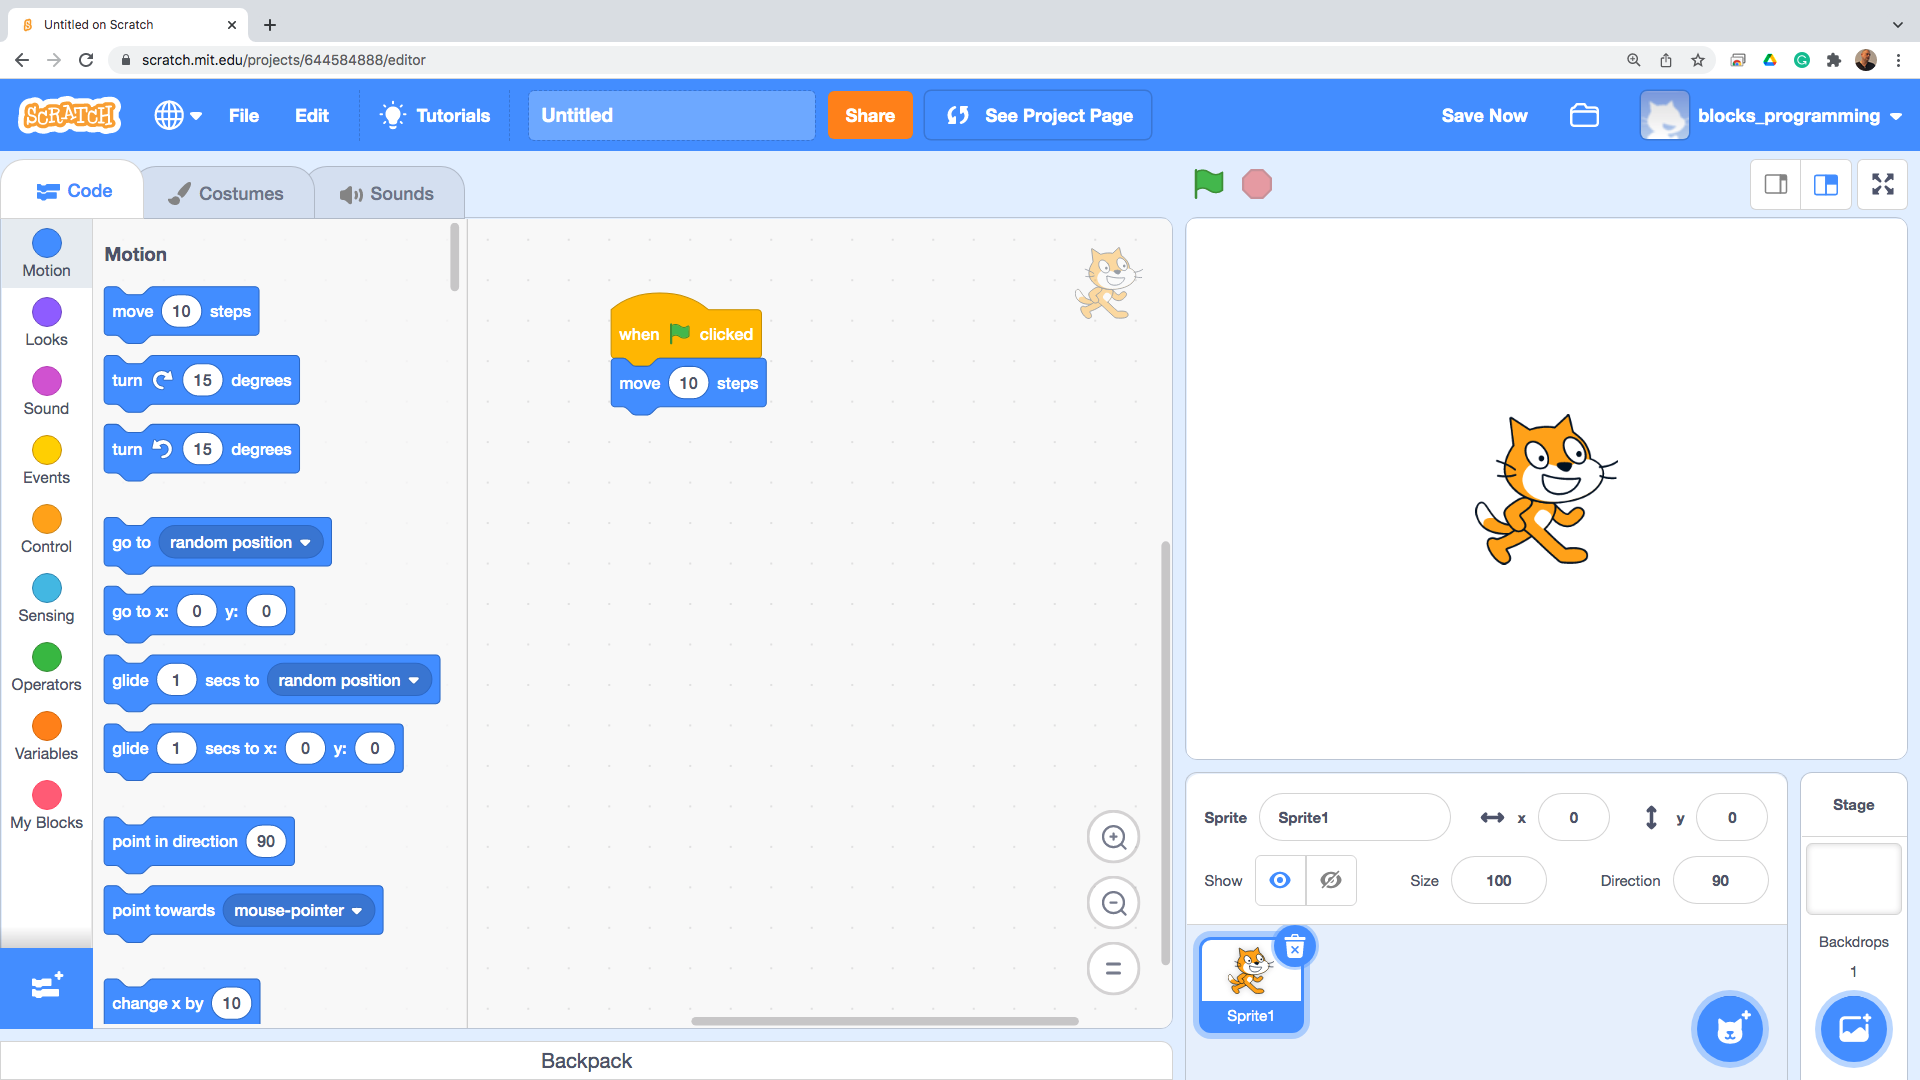
\includegraphics[width=1.0\linewidth,height=0.5\linewidth]{fig010014.png}
   \caption{Step by step instructions}
\label{fig010014}
\end{figure}

After moving the cat sprite, it is crucial to incorporate a waiting pause to make the movement visually noticeable. In Scratch, this can be achieved using the "wait" instruction, which introduces a specified delay before the following action or instruction is executed (Fig. \ref{fig010015}, which cannot be displayed in a text-based format).

By using the "wait" block and specifying the number of seconds or fractions of a second, users can introduce a pause in the program execution. This allows for better control over the timing and synchronization of actions within a project. During the waiting period, the program remains idle, allowing users to observe the effects of previous actions before proceeding to the next step.

Combined with the "move" block, the "wait" block helps create a smoother and more comprehensible visual experience in Scratch projects, providing time for movements or changes to be observed and appreciated.

\begin{figure}[H]
   \centering
   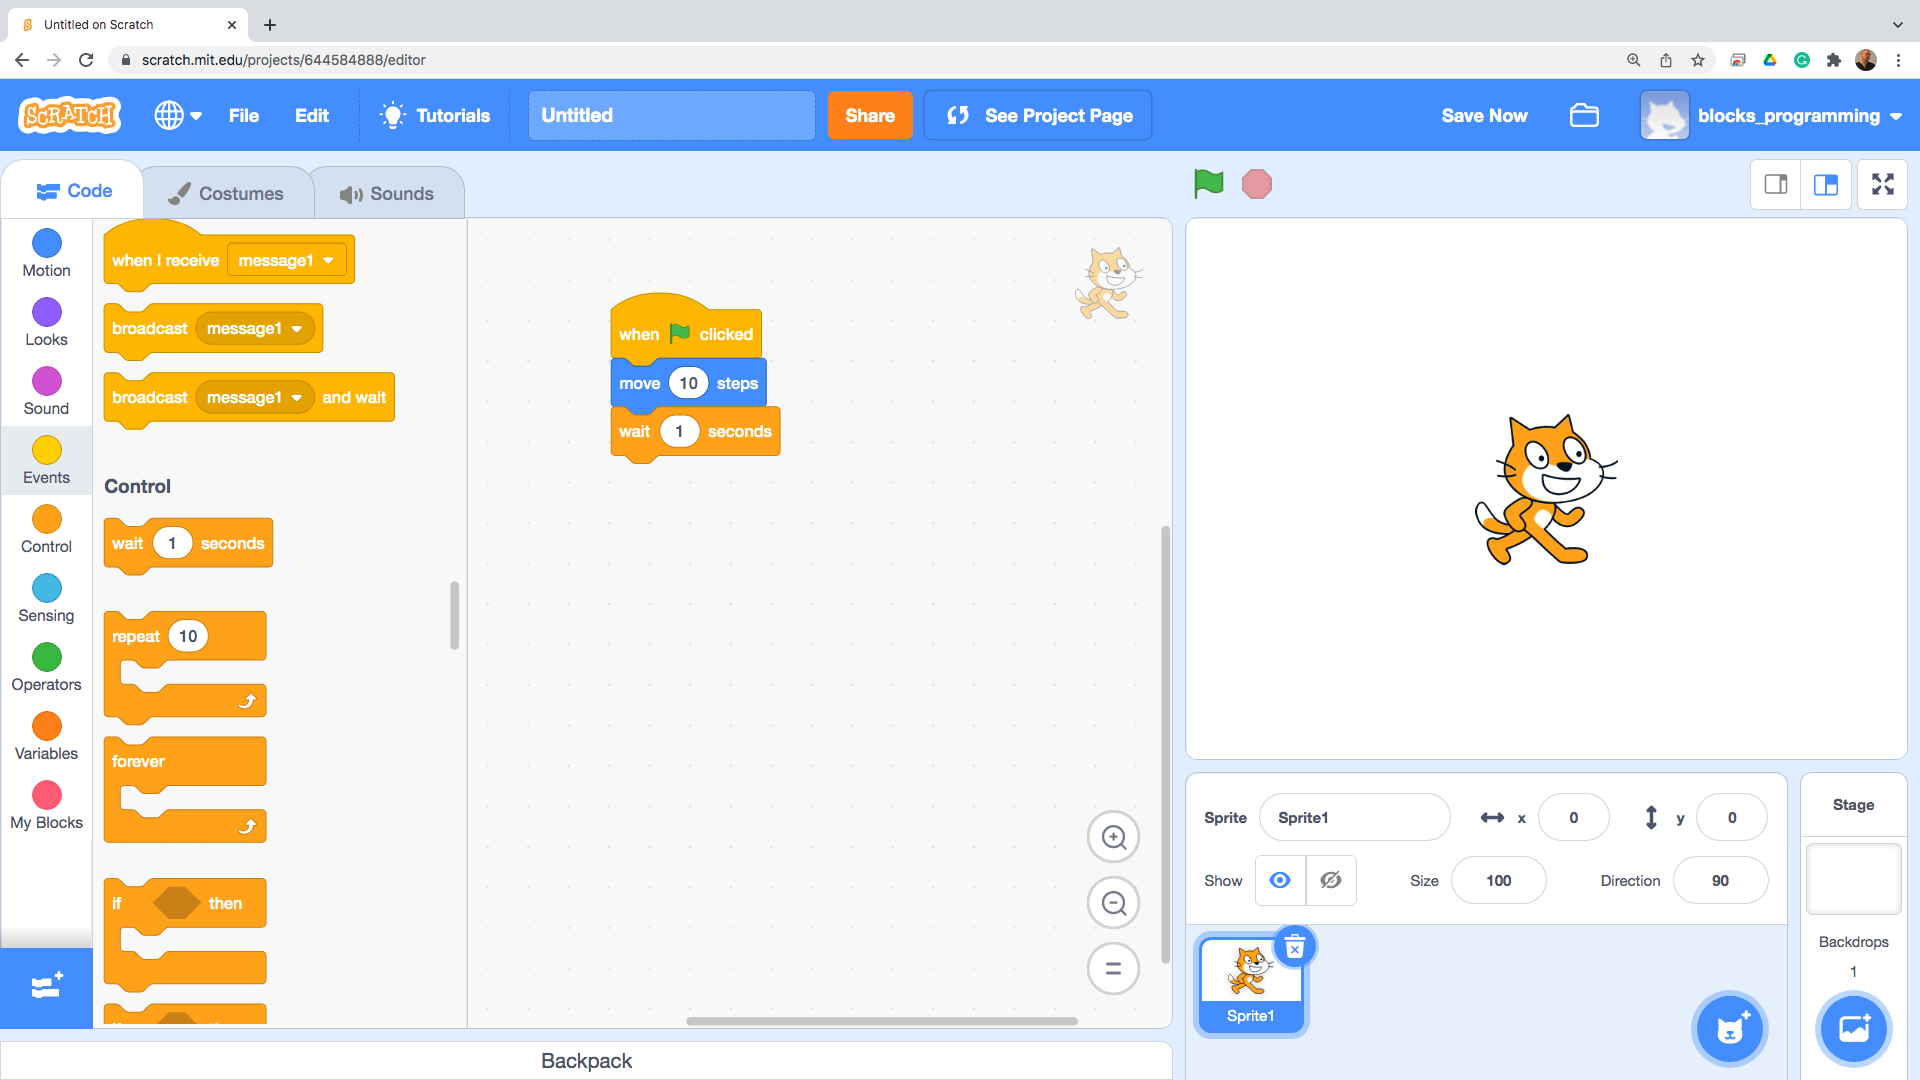
\includegraphics[width=1.0\linewidth,height=0.5\linewidth]{fig010015.png}
   \caption{Wait instruction}
\label{fig010015}
\end{figure}

After the waiting period, if you want the cat sprite to return to its original position, you can achieve this by executing a move instruction with a negative number of steps (Fig. \ref{fig010016}, which cannot be displayed in a text-based format).

In Scratch, when a negative value is provided in the "move" block, it instructs the sprite to move in the opposite direction of the positive value. The cat sprite will move back to its original position by specifying a negative number of steps, effectively undoing the previous movement.

This technique allows you to create animations or interactions where sprites move forward and return to their starting point. Combining positive and negative values with appropriate wait periods enables you to achieve various visual effects and create engaging experiences within your Scratch projects.

\begin{figure}[H]
   \centering
   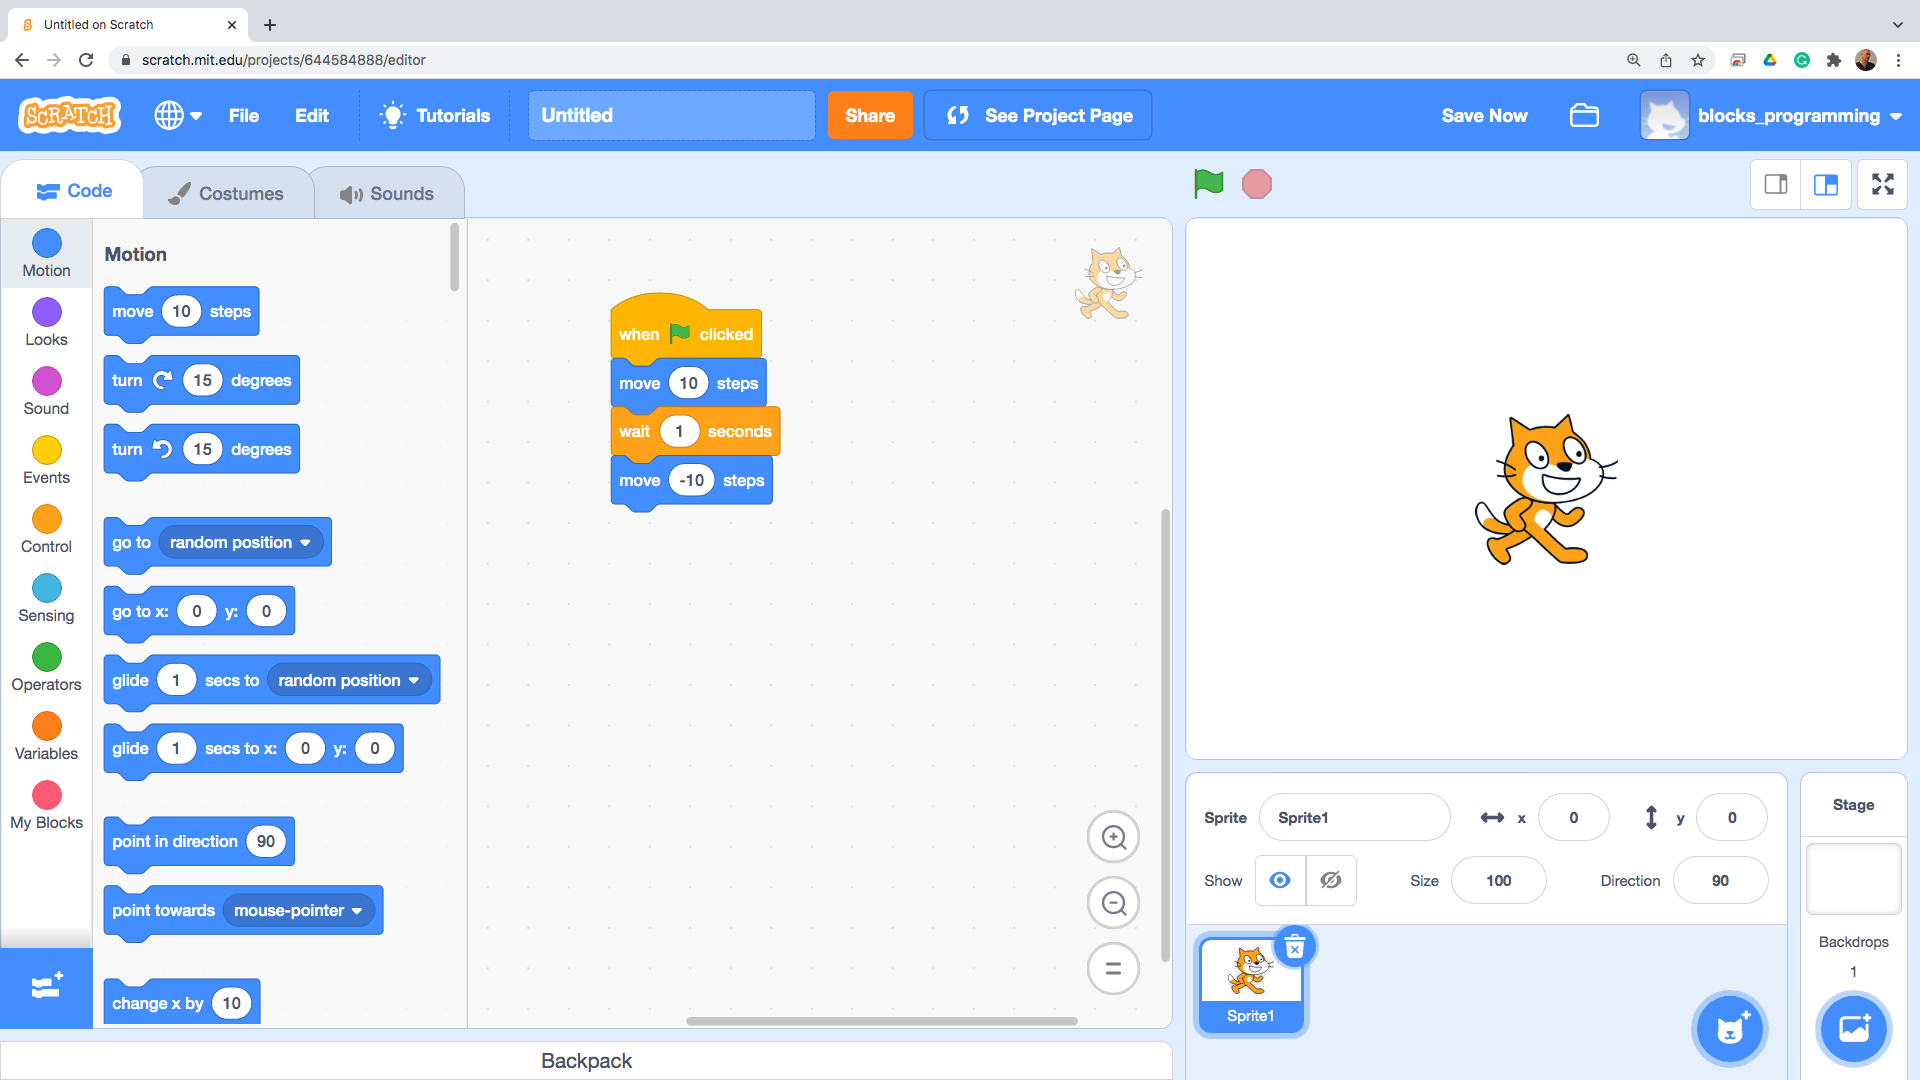
\includegraphics[width=1.0\linewidth,height=0.5\linewidth]{fig010016.png}
   \caption{Instructions for moving back}
\label{fig010016}
\end{figure}

Once all the desired instructions have been executed in a Scratch program, it is necessary to end the program. For this purpose, Scratch provides a separate block in the list of instructions known as the "end" block (Fig. \ref{fig010017}, which cannot be displayed in a text-based format).

The "end" block serves as the final instruction in a Scratch program, indicating that the program execution should cease at that point. When the program reaches the "end" block, all actions and instructions will halt and no longer continue running.

Including the "end" block in your program ensures proper termination and prevents unintended behavior or infinite loops. It allows you to control the execution flow and explicitly define the end point of your program in Scratch.

\begin{figure}[H]
   \centering
   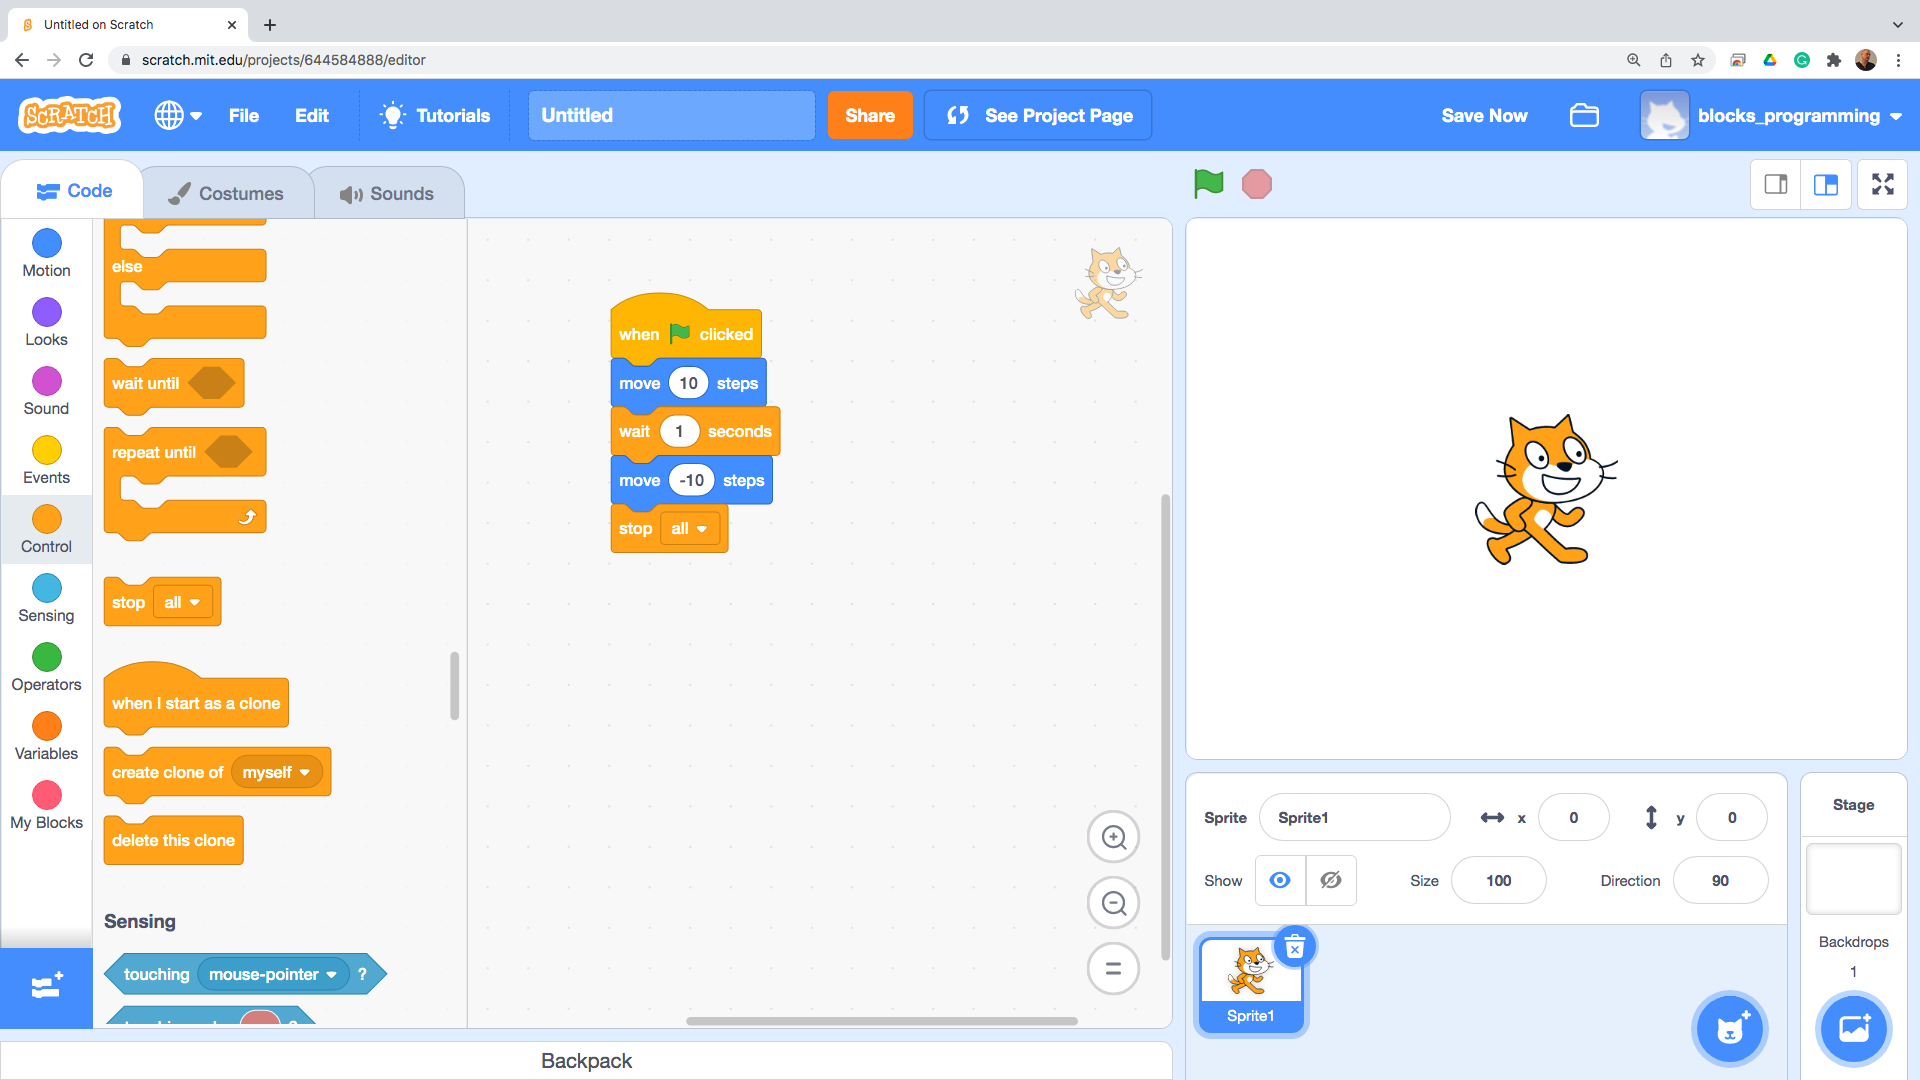
\includegraphics[width=1.0\linewidth,height=0.5\linewidth]{fig010017.png}
   \caption{End instruction}
\label{fig010017}
\end{figure}

The program you have written in Scratch can be executed by pressing the green flag button (Fig. \ref{fig010018}, which cannot be displayed in a text-based format). When the green flag is clicked, the program will start running, and your written instructions will be executed in sequence.

If you need to stop the program immediately during its execution, Scratch provides an emergency stop button with a red circle to the right of the green flag button. Clicking the red circle will halt the program's execution and bring it to a stop.

These buttons give you control over the start and stop of your program, allowing you to test and observe the behavior of your project. The green flag initiates the program, while the red circle provides a means to interrupt the program's execution if necessary.

\begin{figure}[H]
   \centering
   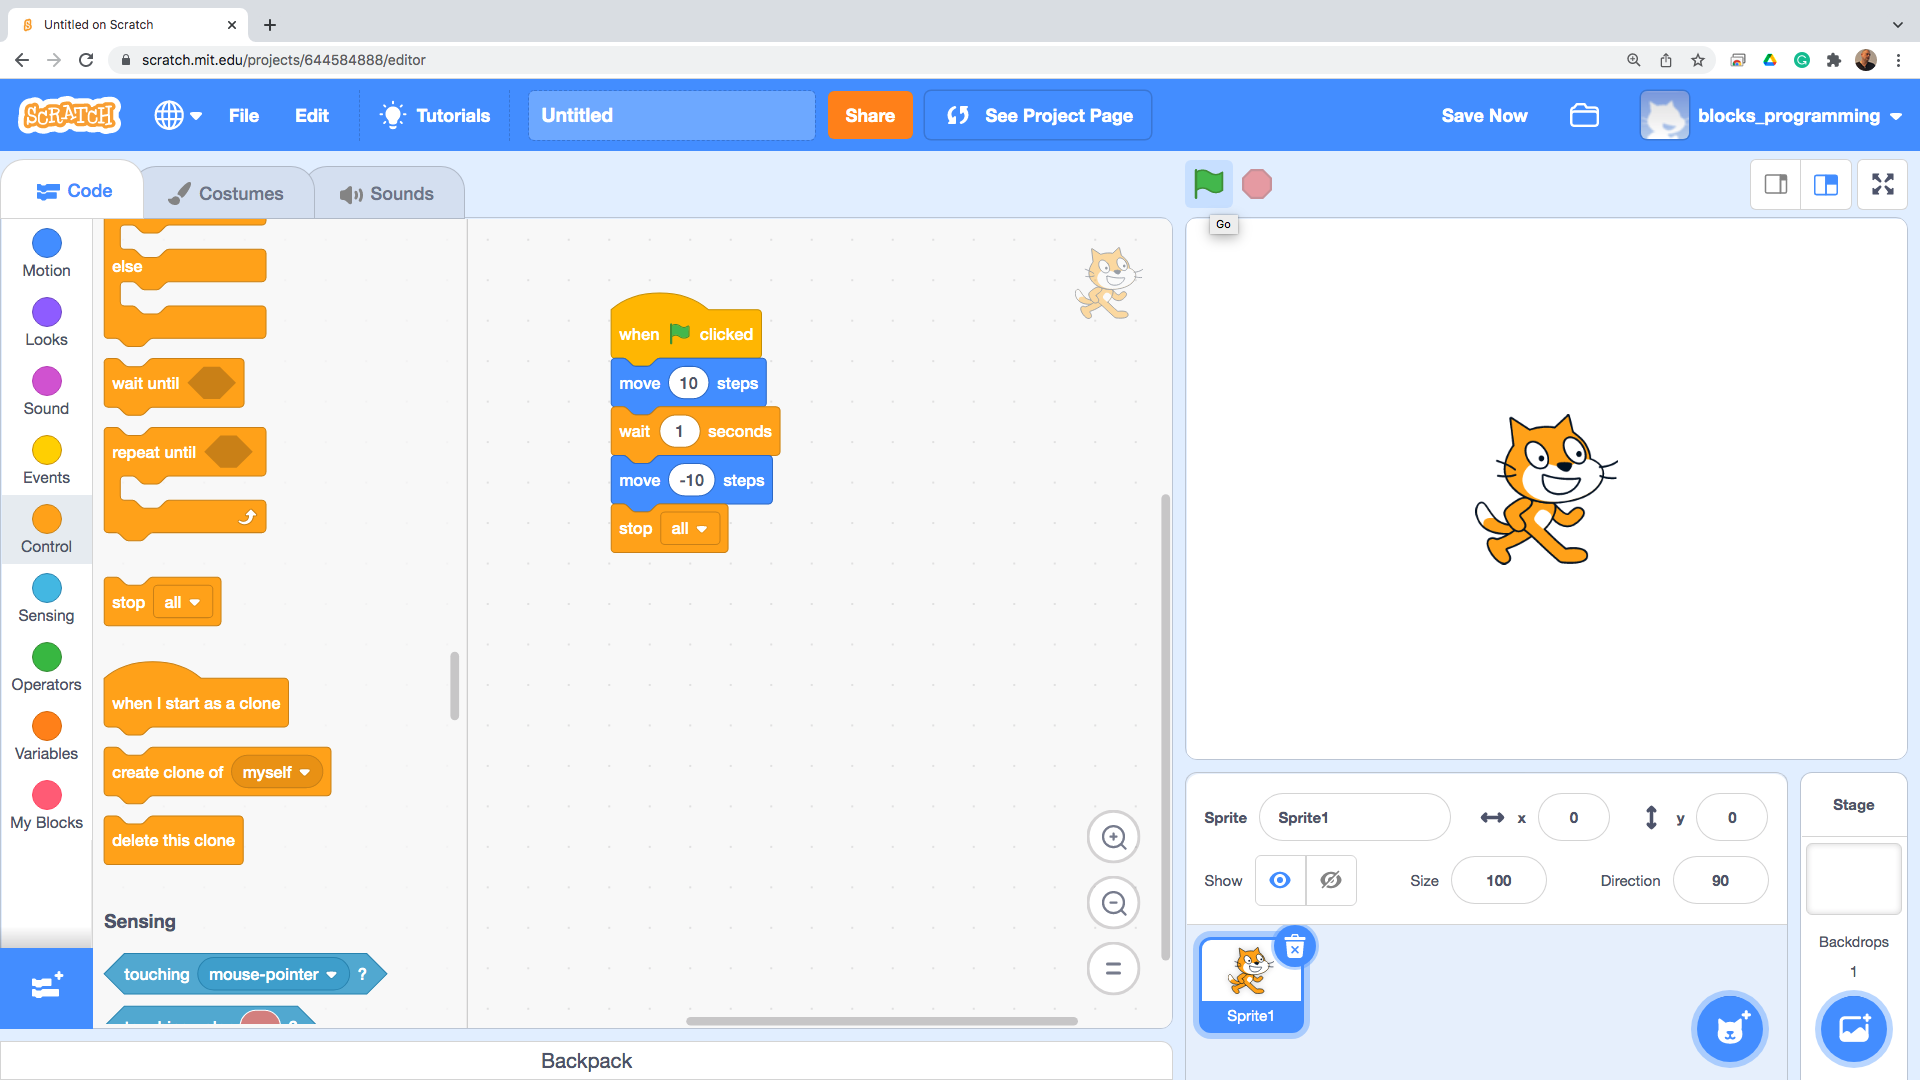
\includegraphics[width=1.0\linewidth,height=0.5\linewidth]{fig010018.png}
   \caption{Program Execution}
\label{fig010018}
\end{figure}

When using Scratch, each program you write is organized as a separate project. To access and manage your projects, you can use the "My Stuff" menu, which is part of the options available for registered users (Fig. \ref{fig010019}, which cannot be displayed in a text-based format).

The "My Stuff" menu provides a centralized location to view and manage your projects. From this menu, you can access your saved projects, create new projects, delete or rename existing projects, and perform other project-related actions.

By navigating to the "My Stuff" menu, you can easily keep track of your Scratch projects and conveniently work on multiple projects or revisit previously created ones. It provides a user-friendly interface to organize and handle your projects within the Scratch environment.

\begin{figure}[H]
   \centering
   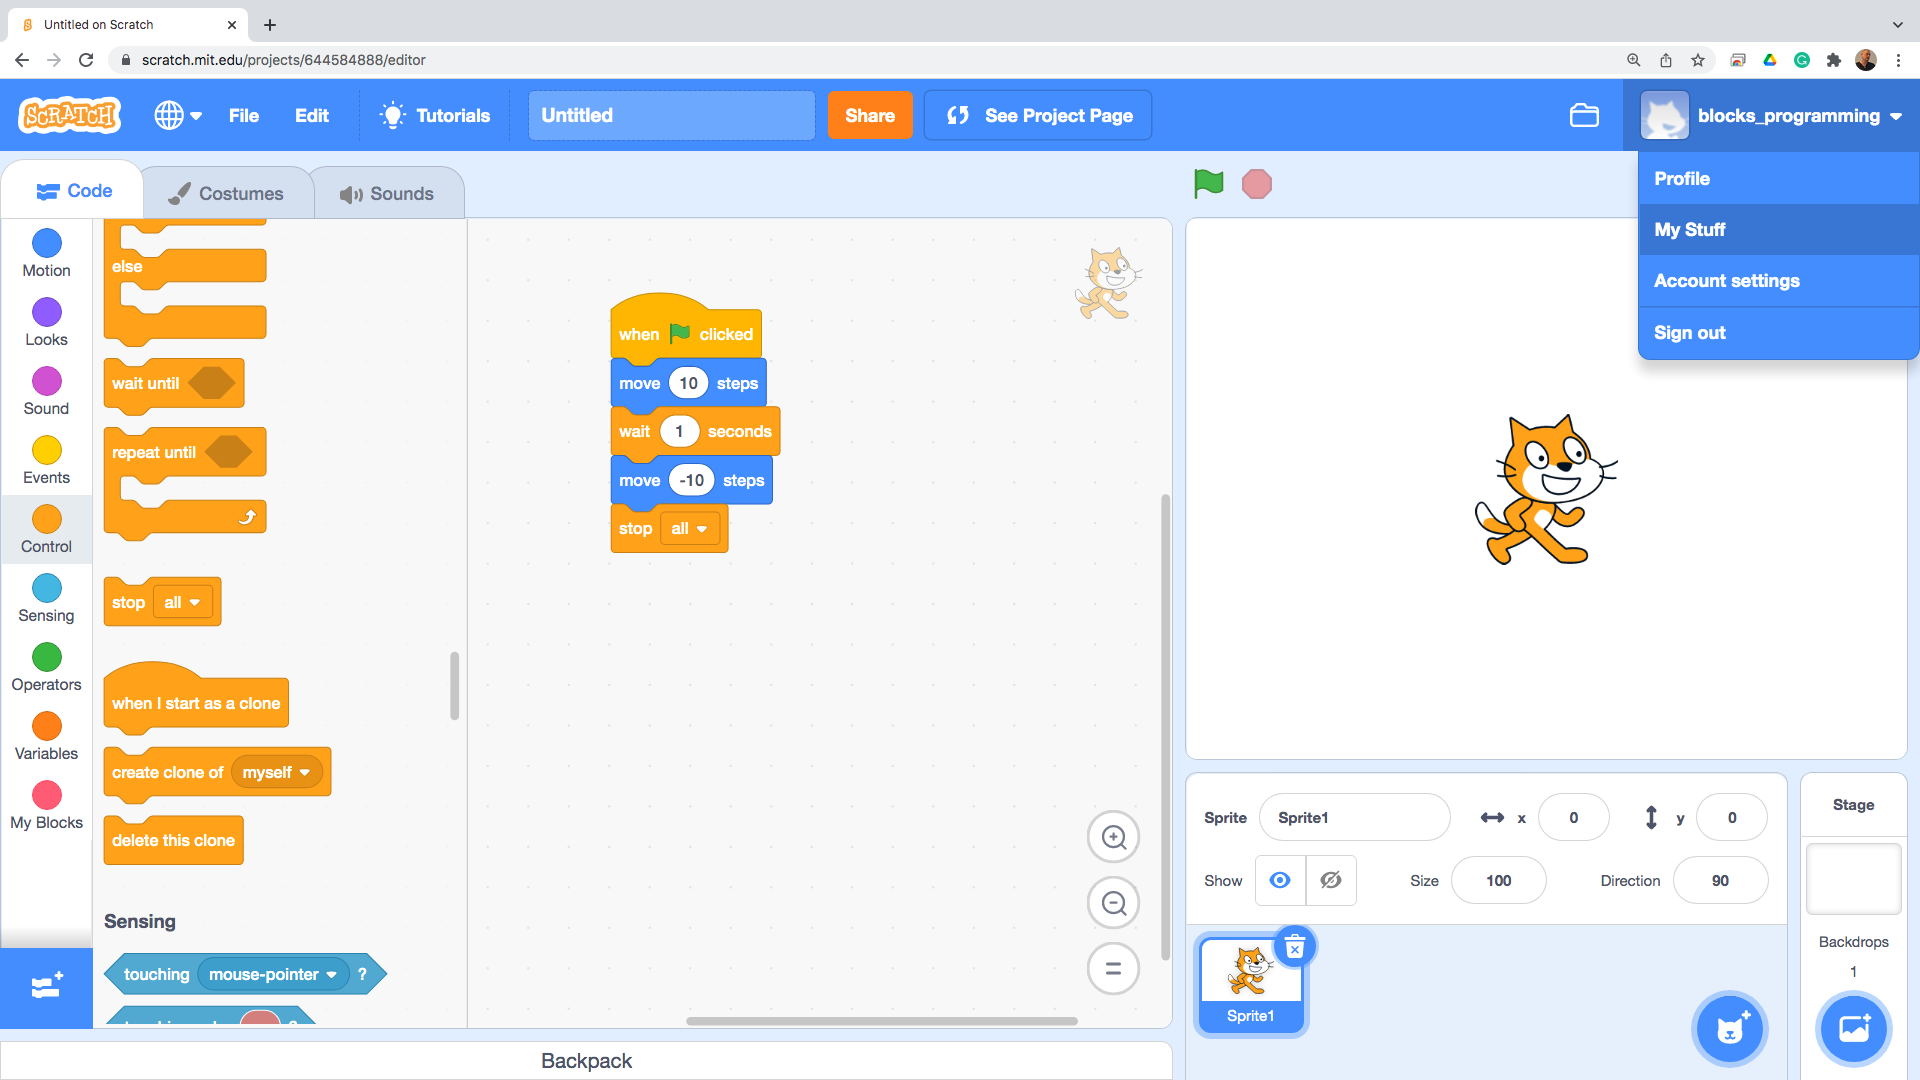
\includegraphics[width=1.0\linewidth,height=0.5\linewidth]{fig010019.png}
   \caption{Project Organization Menu}
\label{fig010019}
\end{figure}

In Scratch, each project is assigned a working name by default (Fig. \ref{fig010020}, which cannot be displayed in a text-based format). However, users can change the project name as desired, providing a more descriptive or meaningful title that reflects the project's content or purpose.

One of the most appealing advantages of the Scratch programming environment is the ability to share projects with a vast audience. This sharing feature lets users quickly disseminate their knowledge, skills, and creations to others. Users can showcase their work, receive feedback, collaborate with peers, and inspire others to learn and explore programming by sharing projects.

Sharing projects facilitates the transfer of knowledge and skills and enables the assessment and evaluation of the work done. Users can receive comments, suggestions, and appreciation for their projects, fostering community and engagement within the Scratch platform.

The sharing feature in Scratch promotes a collaborative and interactive learning environment where users can learn from one another, exchange ideas, and be recognized for their creativity and accomplishments.

\begin{figure}[H]
   \centering
   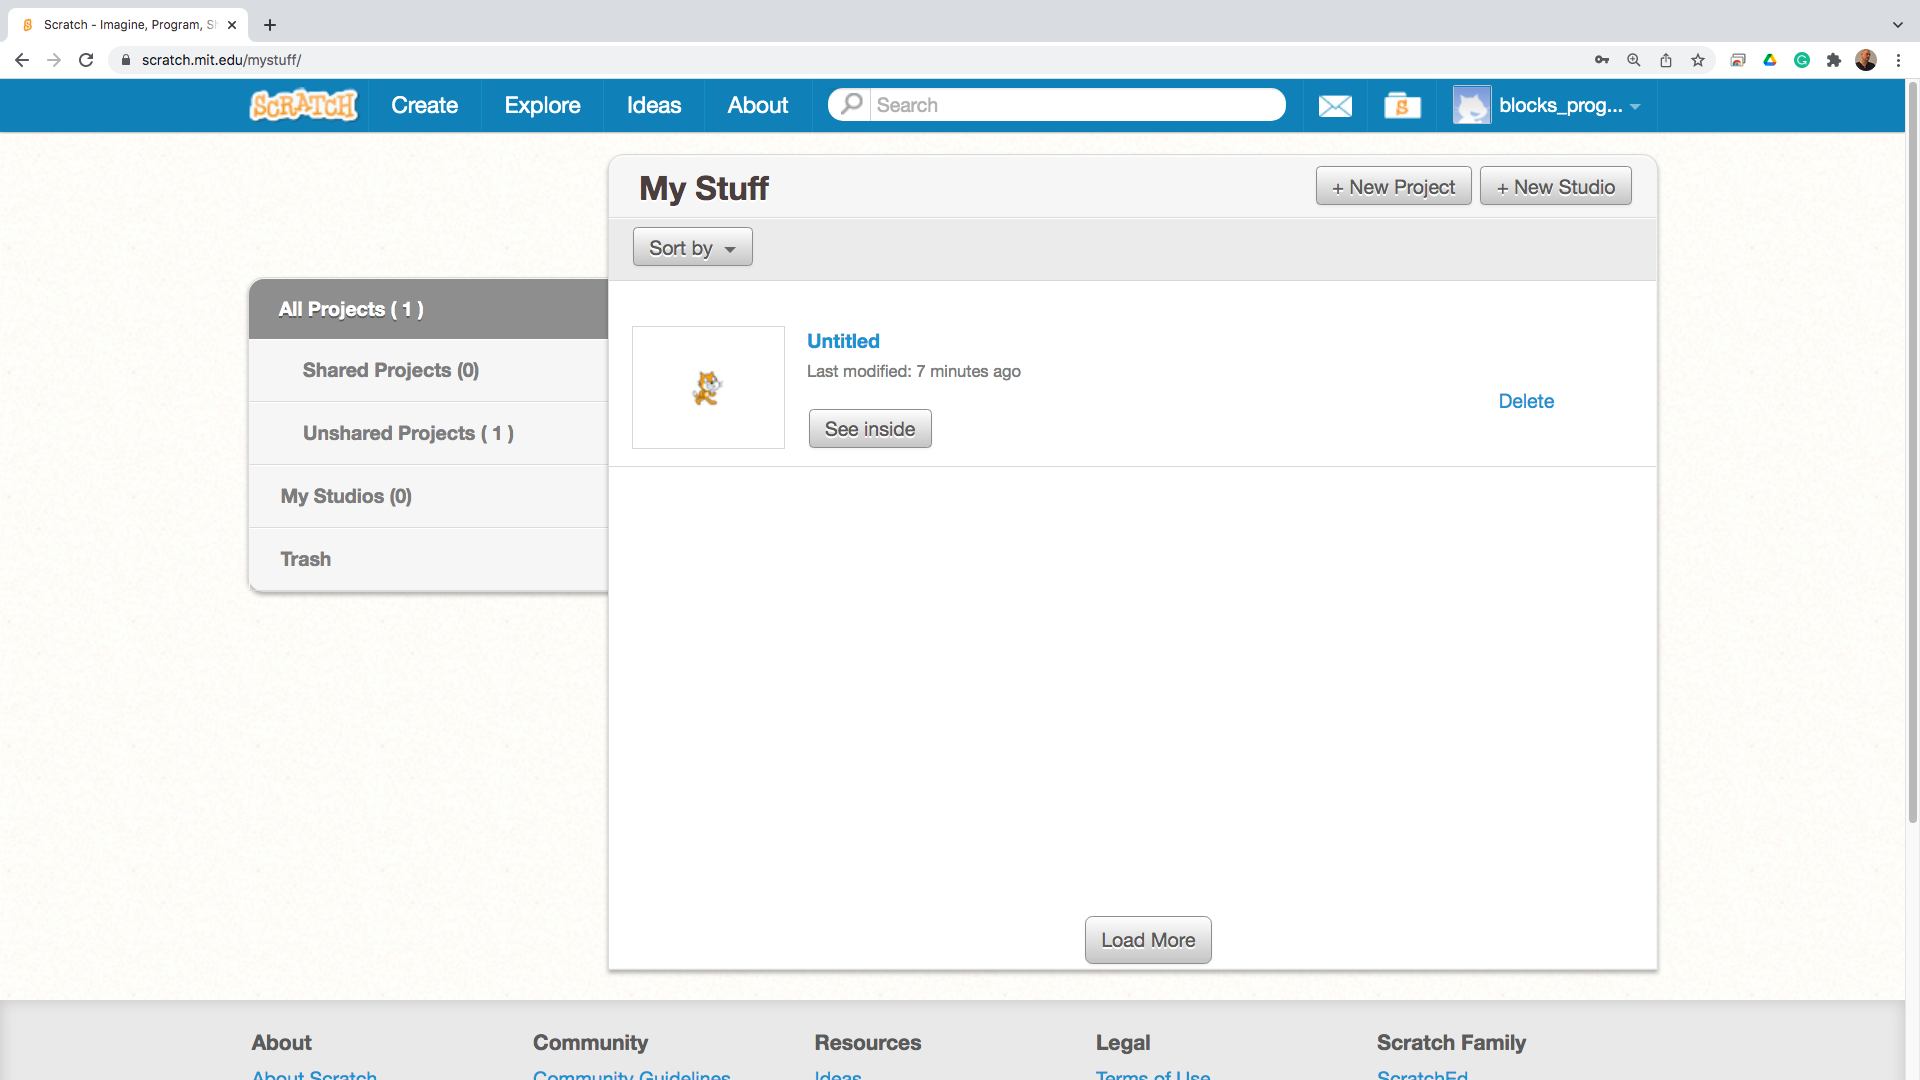
\includegraphics[width=1.0\linewidth,height=0.5\linewidth]{fig010020.png}
   \caption{List of projects}
\label{fig010020}
\end{figure}

One of the most fascinating aspects of block languages is their resemblance to puzzle-solving. Writing instructions and forming a complete program in a block language is akin to assembling puzzle pieces. This characteristic holds particular appeal for children, as many of them enjoy putting together puzzles.

Using colorful blocks and visually appealing elements in block languages adds to their attractiveness. Children are naturally drawn to bright colors and beautiful pictures, and incorporating these elements into programming enhances their engagement and interest. Combining the charm of classic puzzles with the allure of programming can lead to astonishing results.

By presenting programming concepts as puzzles, block languages make the learning experience more enjoyable and accessible for children. It allows them to approach programming as a creative and problem-solving activity, where they can explore and experiment with different combinations of blocks to achieve desired outcomes. This puzzle-like approach promotes critical thinking, logical reasoning, and problem-solving skills engagingly and playfully.

The fusion of puzzle-solving and programming in block languages captivates children's imaginations and motivates them to explore the programming world with enthusiasm and curiosity.

\section{Getting Started in App Inventor}

Working in the App Inventor environment starts by accessing the main web page (Fig. \ref{fig010021}). You can find the App Inventor web page at: \\ \href{https://appinventor.mit.edu/}{https:// appinventor.mit.edu/}

To begin using App Inventor, you must navigate to this web page and load it in your browser. The web page is the entry point to the App Inventor environment, where you can create, design, and develop your mobile applications.

Accessing the App Inventor web page gives you access to a powerful visual programming platform that allows you to build mobile apps using a block-based interface. Whether you're a beginner or have some programming experience, App Inventor provides a user-friendly environment to create functional and interactive mobile applications.

Once you've loaded the main web page, you can explore the various features, resources, and tutorials available on the App Inventor platform to get started with your app development journey.

\begin{figure}[H]
   \centering
   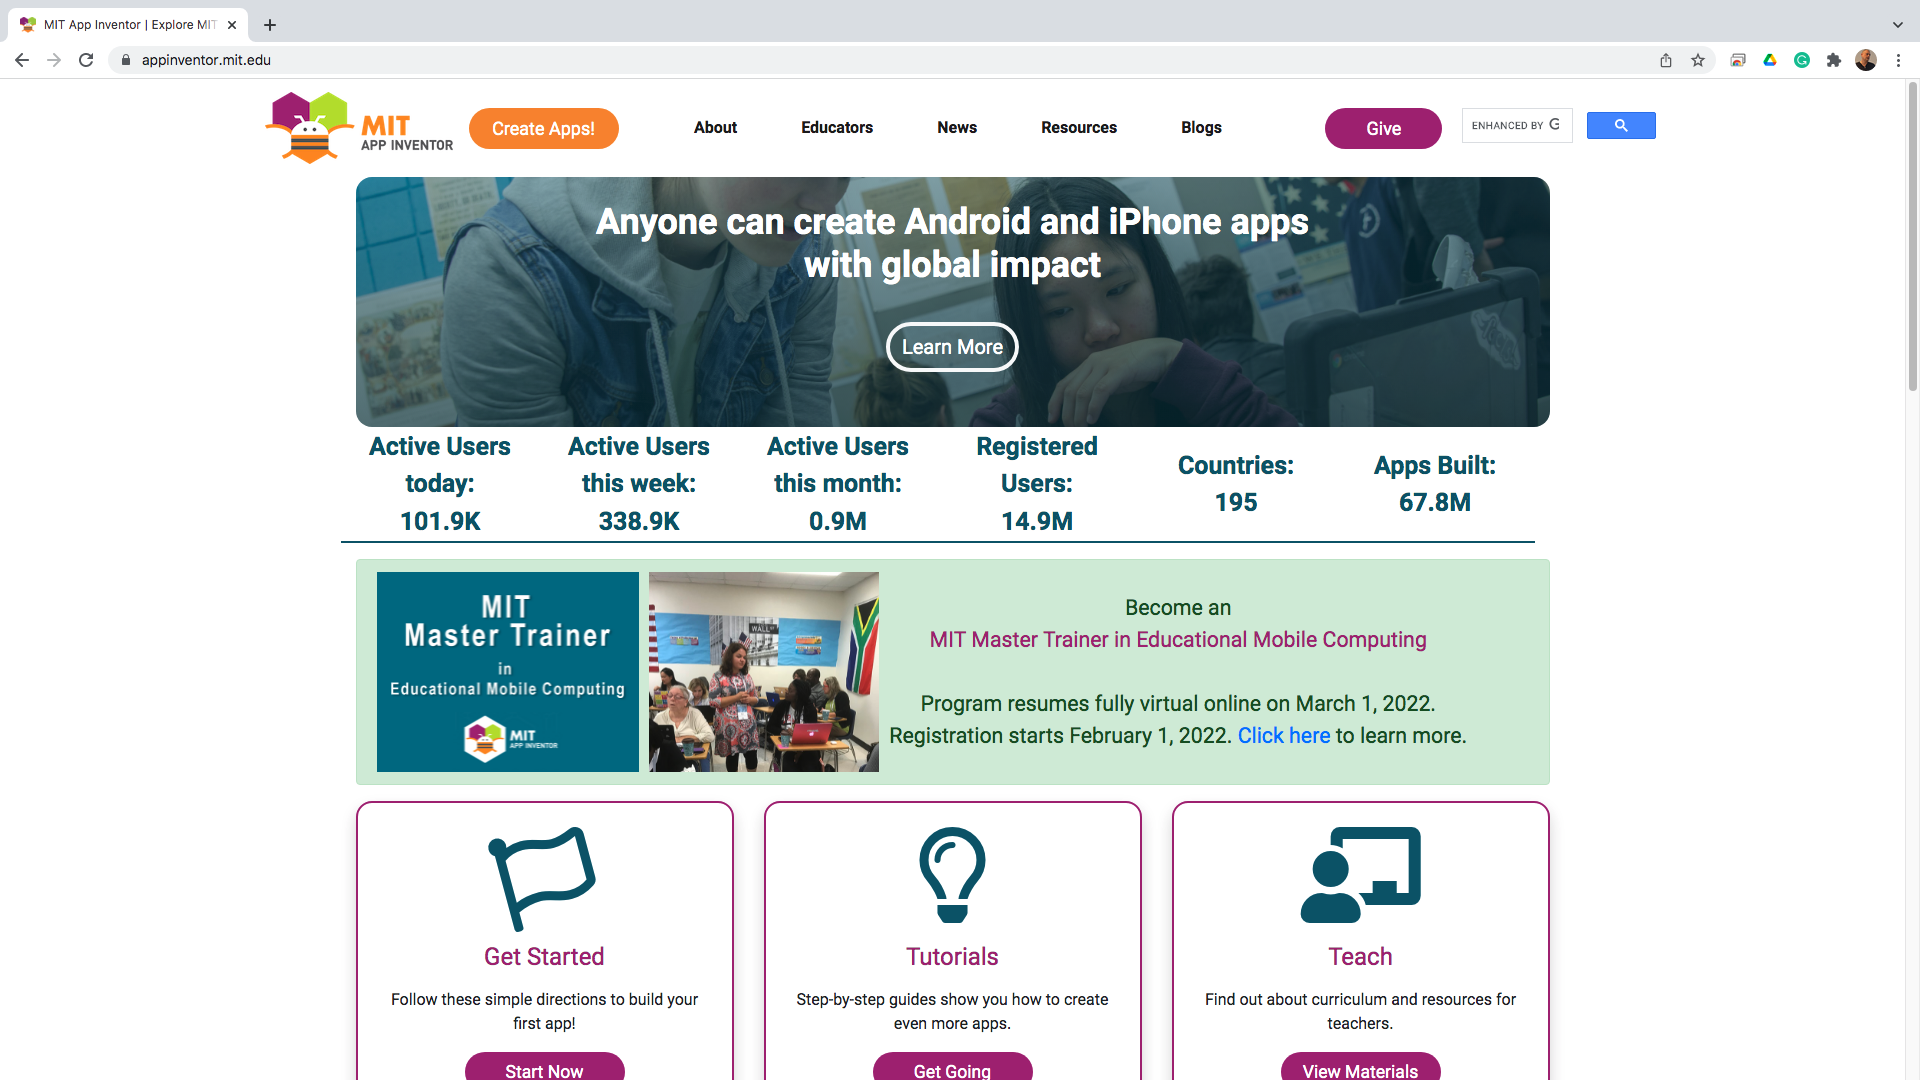
\includegraphics[width=1.0\linewidth,height=0.5\linewidth]{fig010021.png}
   \caption{App Inventor Home Web Page}
\label{fig010021}
\end{figure}

While the Massachusetts Institute of Technology also develops App Inventor, it differs from Scratch in certain aspects. When using App Inventor, you can work with it as a cloud service, and registration is necessary to access its features. However, unlike Scratch, App Inventor provides an alternative method for user registration.

To begin the registration process in App Inventor, you can click on the orange "Create Apps!" button (Fig. \ref{fig010022}), which cannot be displayed in a text-based format. This button initiates the registration procedure and allows you to create your App Inventor account.

Unlike the traditional creation of a user profile, App Inventor allows logging in using a Google account. By choosing this method, you can utilize your existing Gmail credentials for authentication, making the registration process more streamlined and convenient.

Following the prompts after clicking the "Create Apps!" button will guide you through the necessary steps to create your App Inventor account. This process allows you to leverage the cloud-based features of App Inventor and start developing your mobile applications.

\begin{figure}[H]
   \centering
   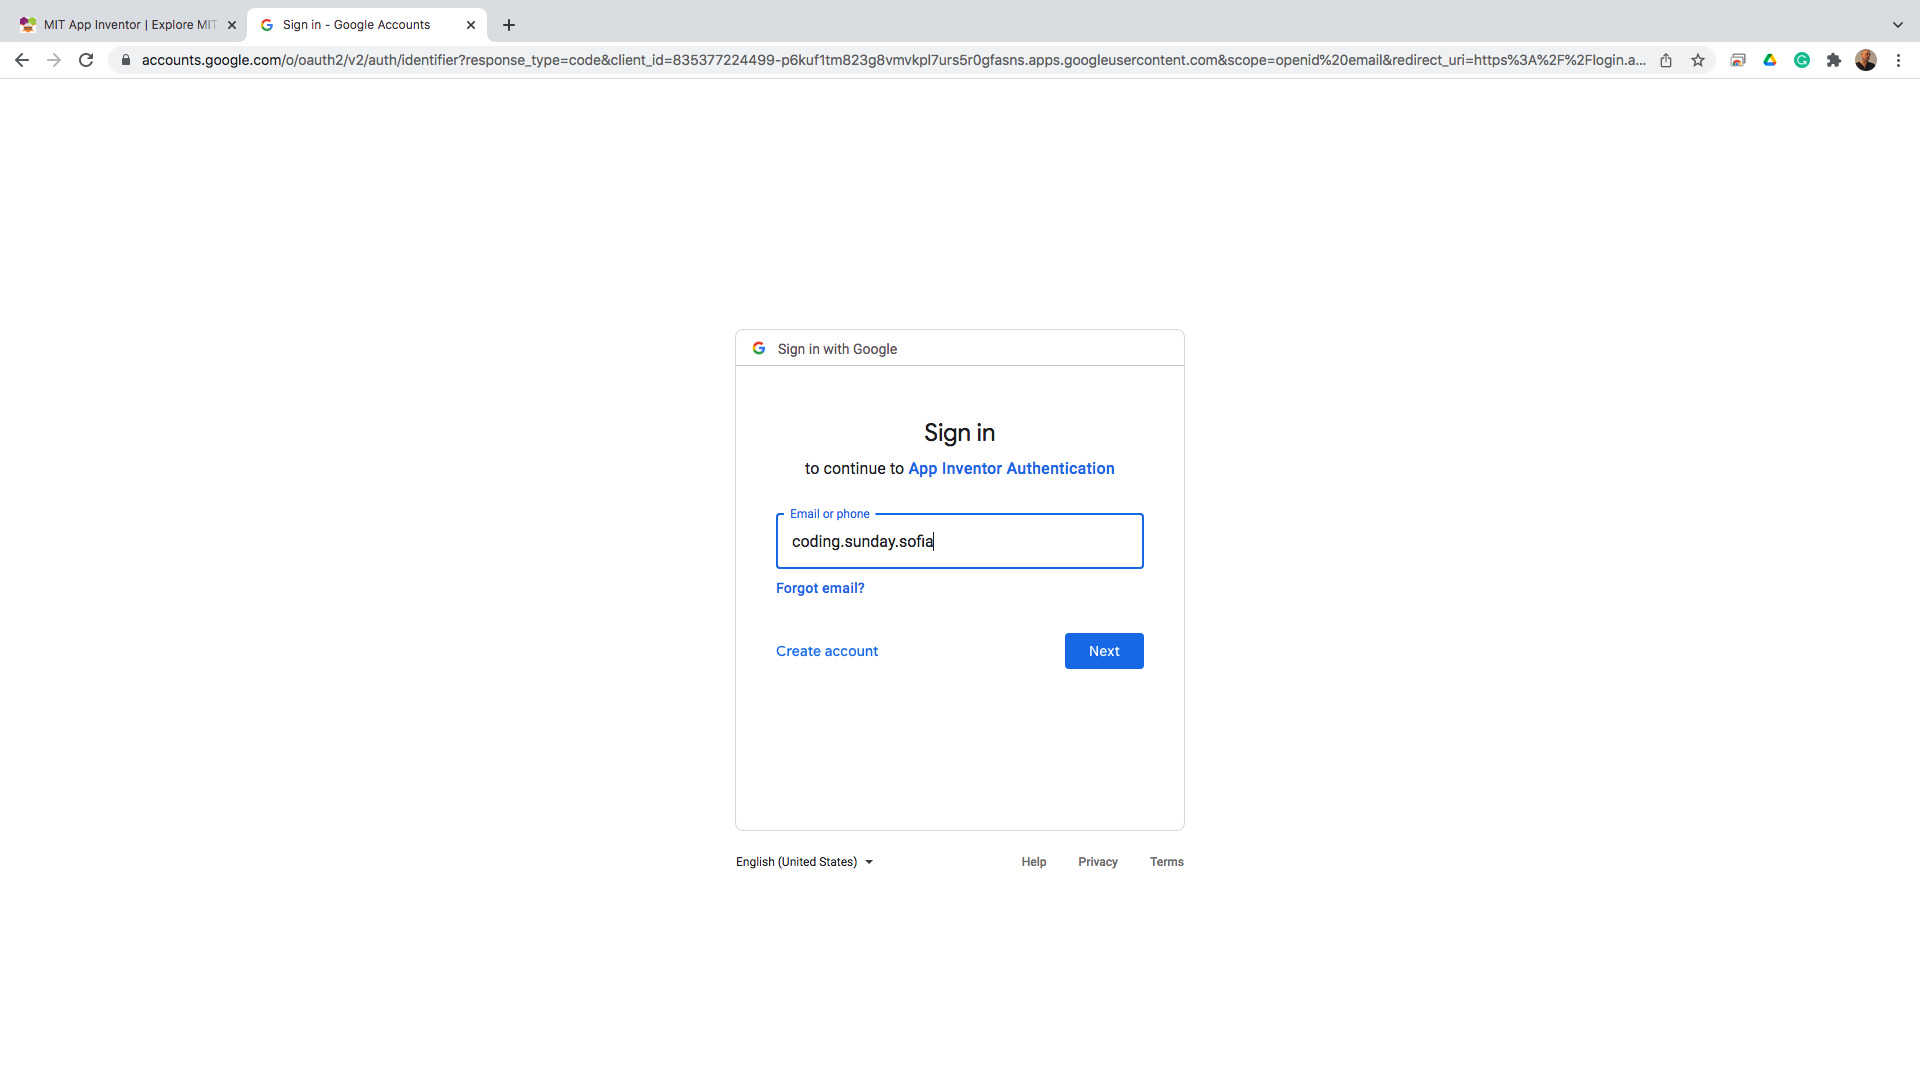
\includegraphics[width=1.0\linewidth,height=0.5\linewidth]{fig010022.png}
   \caption{Choosing a GMail user to log in}
\label{fig010022}
\end{figure}

Once you have selected a user to work within the App Inventor environment, you must authenticate yourself by entering a password (Fig. \ref{fig010023}, which cannot be displayed in a text-based format). This step ensures the security and privacy of your App Inventor account.

After selecting the user, you will be prompted to enter the associated password. This password should correspond to the account you use for App Inventor, whether it is a password specific to App Inventor or your Gmail password if you log in through your Google account.

You will successfully authenticate and gain access to your App Inventor account by providing the correct password. This authentication process verifies your identity and allows you to continue working within the App Inventor environment to create and develop mobile applications.

Keeping your password secure and confidential is essential to protect your account from unauthorized access.

\begin{figure}[H]
   \centering
   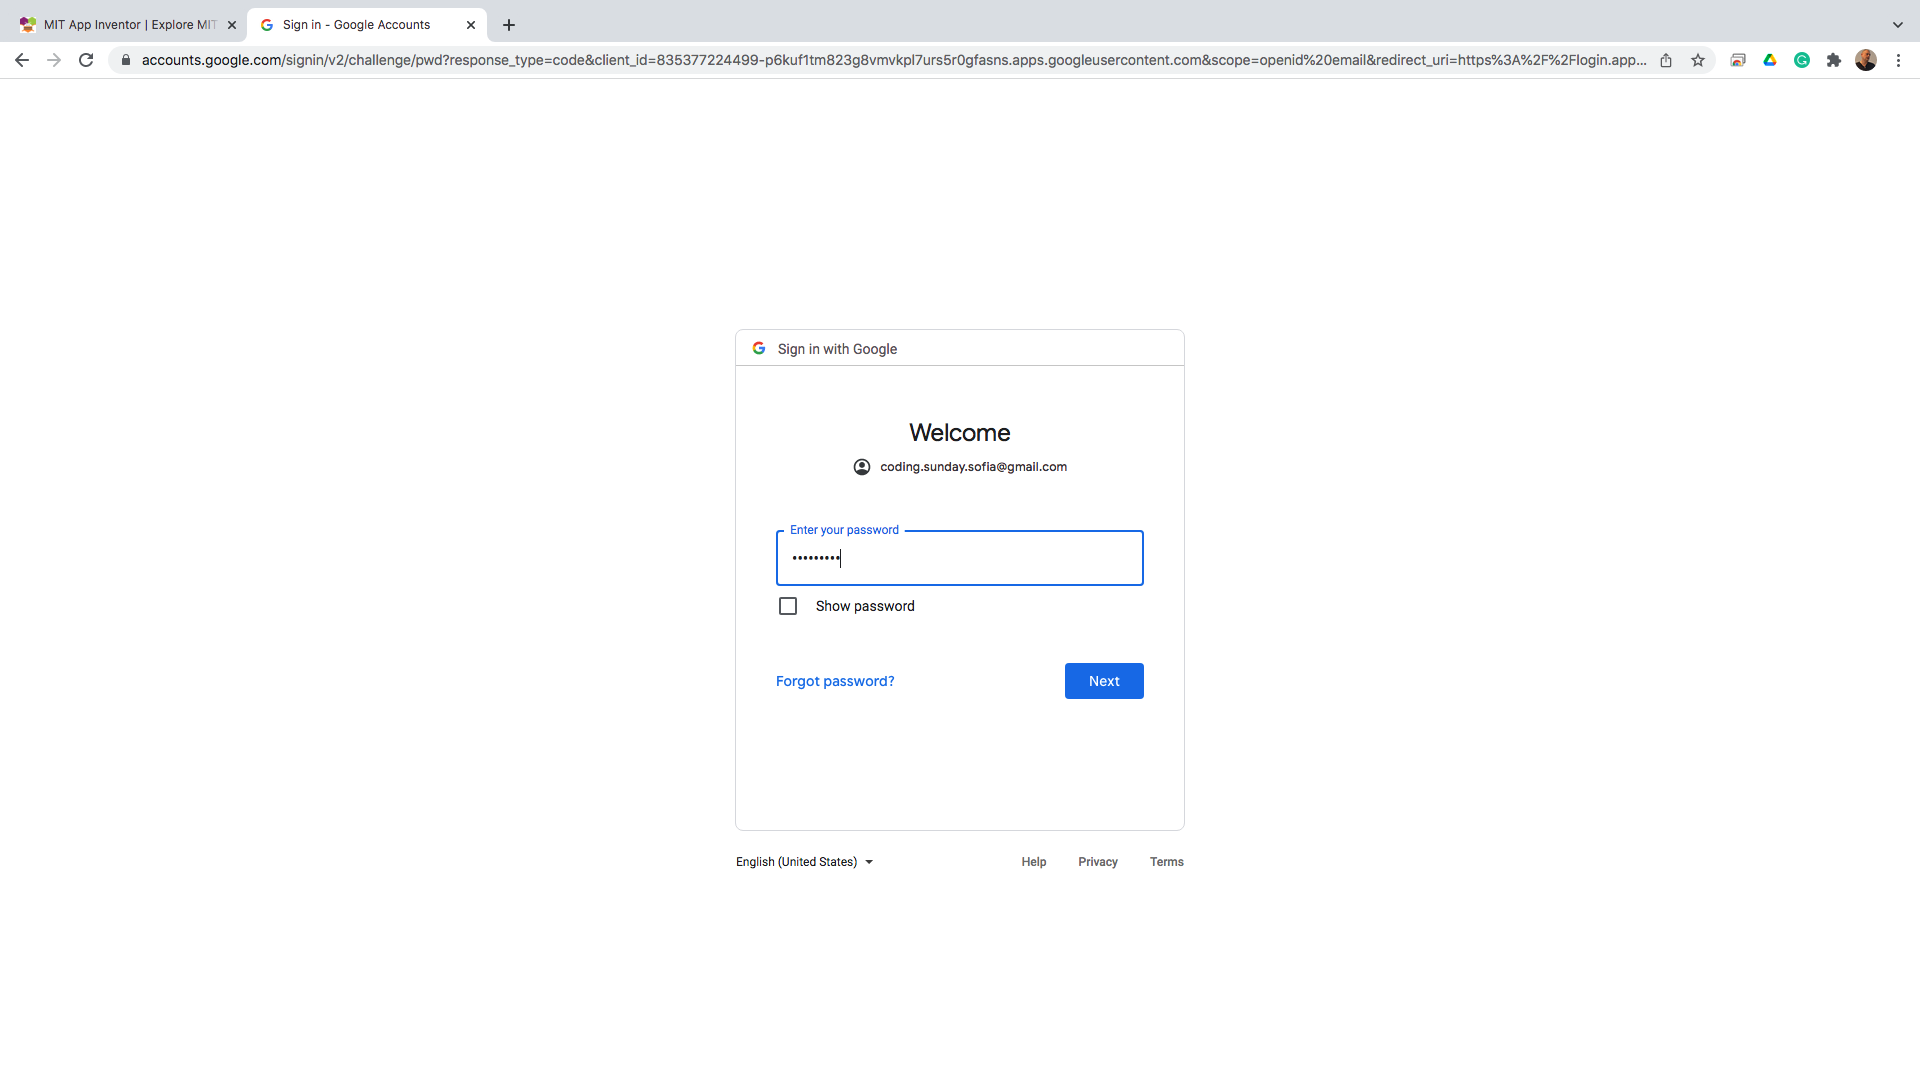
\includegraphics[width=1.0\linewidth,height=0.5\linewidth]{fig010023.png}
   \caption{User Authentication}
\label{fig010023}
\end{figure}

To work in the App Inventor programming environment, users must agree to the general terms and conditions of the platform (Fig. \ref{fig010024}, which cannot be displayed in a text-based format). This step ensures that users are aware of and agree to comply with the rules and guidelines set forth by App Inventor.

Upon accessing the App Inventor platform, users will be presented with the general terms and conditions that outline the rights and responsibilities of both the users and the platform. These terms typically cover aspects such as acceptable use, intellectual property rights, data privacy, and any specific policies or guidelines that must be followed.

To proceed with using App Inventor, users are required to read and accept these terms and conditions. This confirms their agreement to abide by the platform's rules and regulations. It is essential to carefully review the terms and seek clarification before accepting them.

By agreeing to the general terms of the platform, users can continue with their App Inventor experience and leverage the tools and resources provided to create and develop their mobile applications.

\begin{figure}[H]
   \centering
   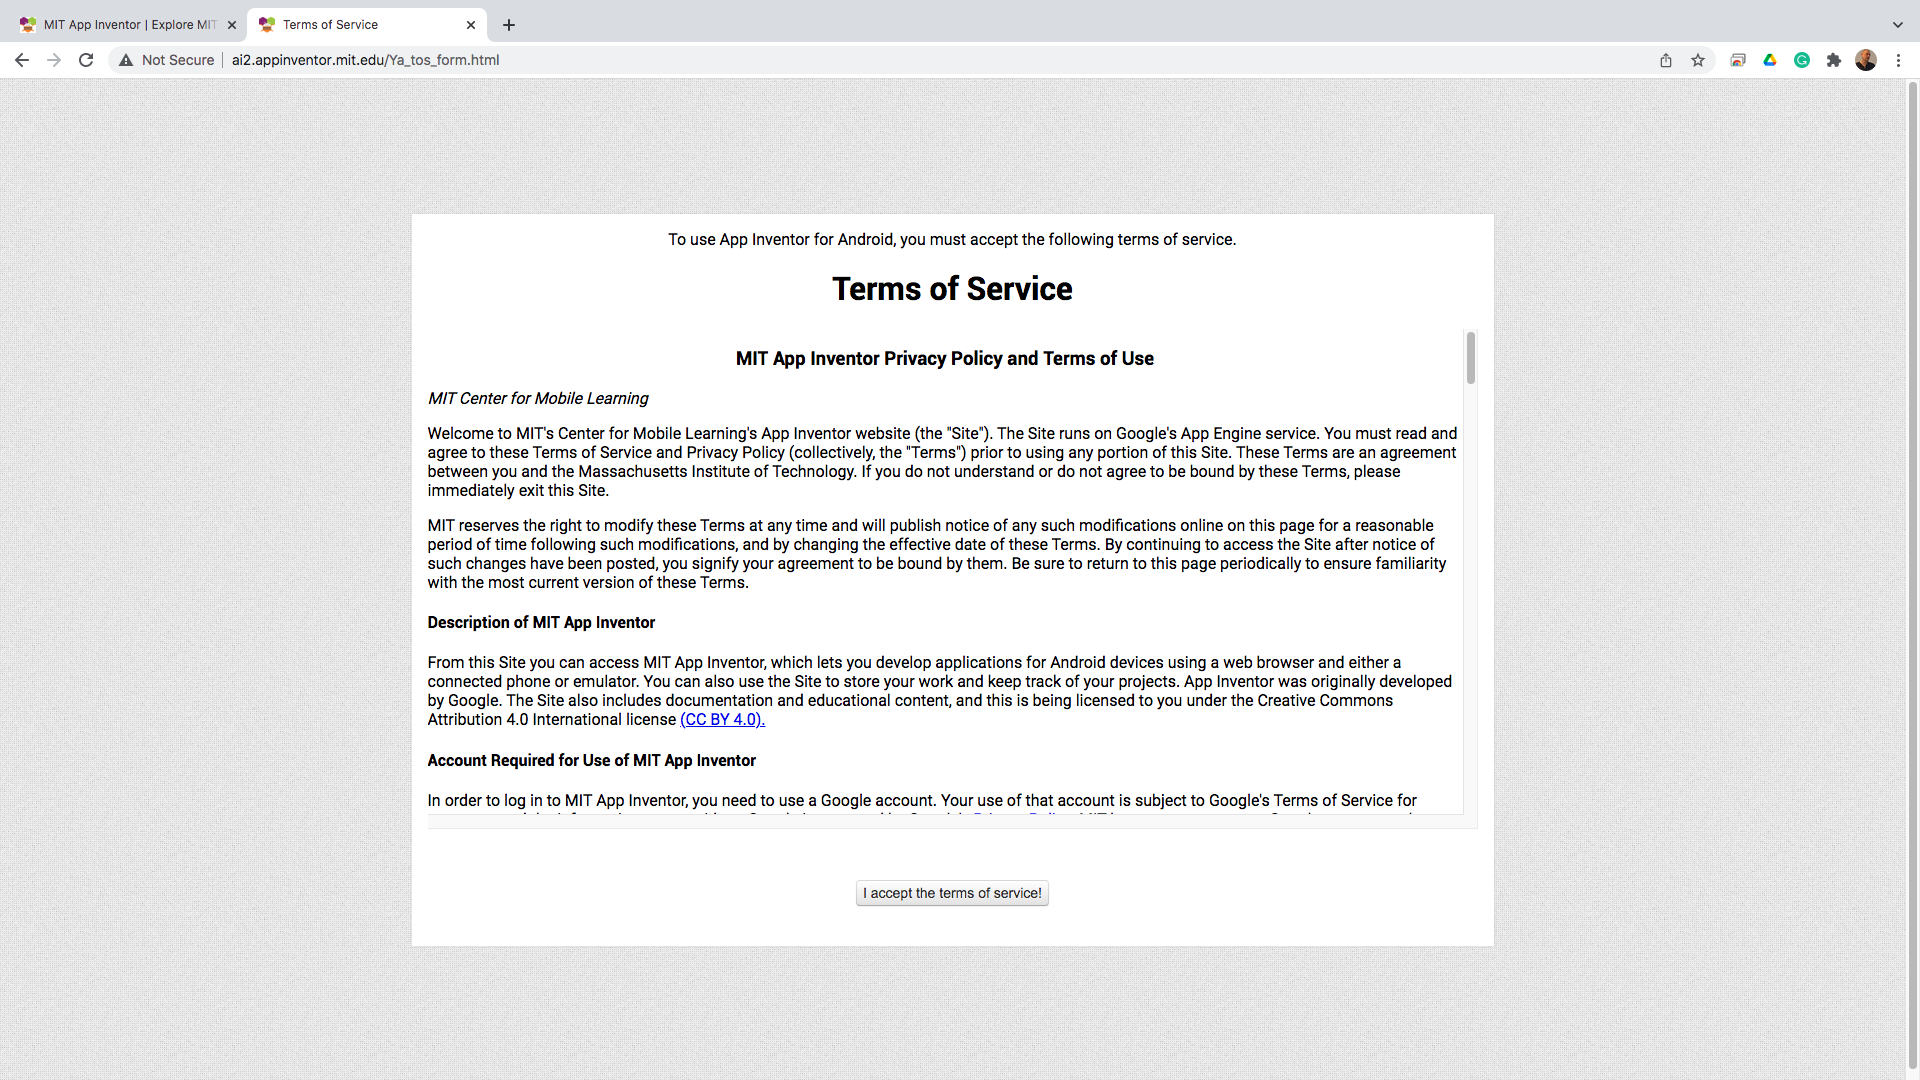
\includegraphics[width=1.0\linewidth,height=0.5\linewidth]{fig010024.png}
   \caption{General Terms of Use of the Program Environment}
\label{fig010024}
\end{figure}

After completing the necessary steps to enter the App Inventor programming environment, the process culminates with a welcome web page (Fig. \ref{fig010025}), which provides more detailed information about the program environment, the type of instance launched, and the version.

You will find valuable information regarding the App Inventor programming environment on the welcome web page. This includes details about the features, functionalities, and tools available within the platform. The page may also provide information about any updates or improvements in the current version of App Inventor.

Additionally, the welcome web page may display the type of instance that has been launched, which could be specific to your account or project settings. This information helps identify the configuration you are currently working with within App Inventor.

By presenting this detailed information, the welcome web page offers an overview of the program environment and sets the stage for your App Inventor experience. It serves as a helpful reference for understanding the capabilities and specifications of the programming environment you are about to engage with.

\begin{figure}[H]
   \centering
   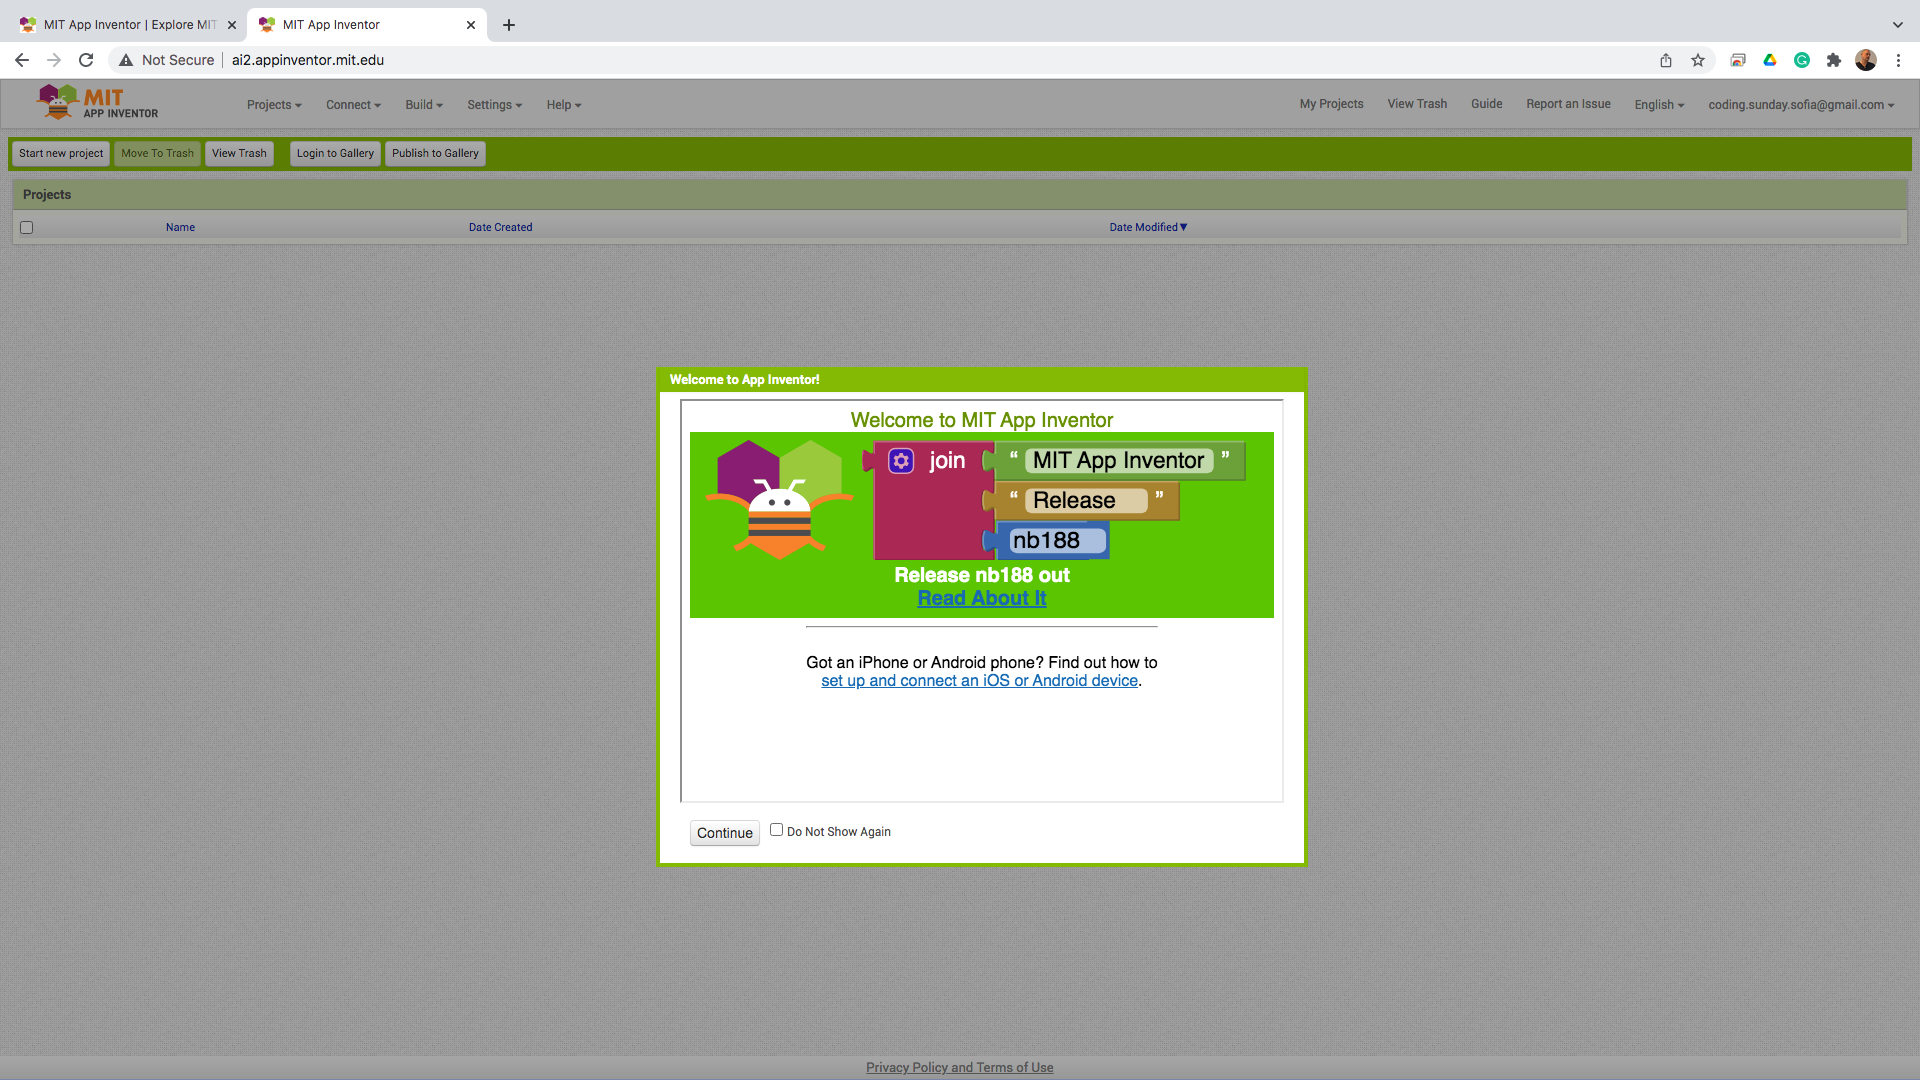
\includegraphics[width=1.0\linewidth,height=0.5\linewidth]{fig010025.png}
   \caption{Welcome Page}
\label{fig010025}
\end{figure}

Upon entering the App Inventor programming environment, users are presented with several options, including the opportunity to view various learning projects that serve as an initial introduction to working with the programming environment (Fig. \ref{fig010026}, which cannot be displayed in a text-based format).

These learning projects are designed to provide users, especially beginners, with hands-on examples and demonstrations of how the programming environment functions. By exploring these projects, users can better understand the App Inventor interface, the components available for building mobile applications, and the logic behind creating functional apps.

These learning projects often cover various topics, from basic app development concepts to more advanced functionalities. They serve as a starting point for users to familiarize themselves with the App Inventor environment, its features, and the overall app creation process.

By selecting this option, users can browse through the collection of learning projects and explore them at their own pace. It is an excellent way to gain practical experience and learn by example, providing a foundation for further exploration and development within the App Inventor programming environment.

\begin{figure}[H]
   \centering
   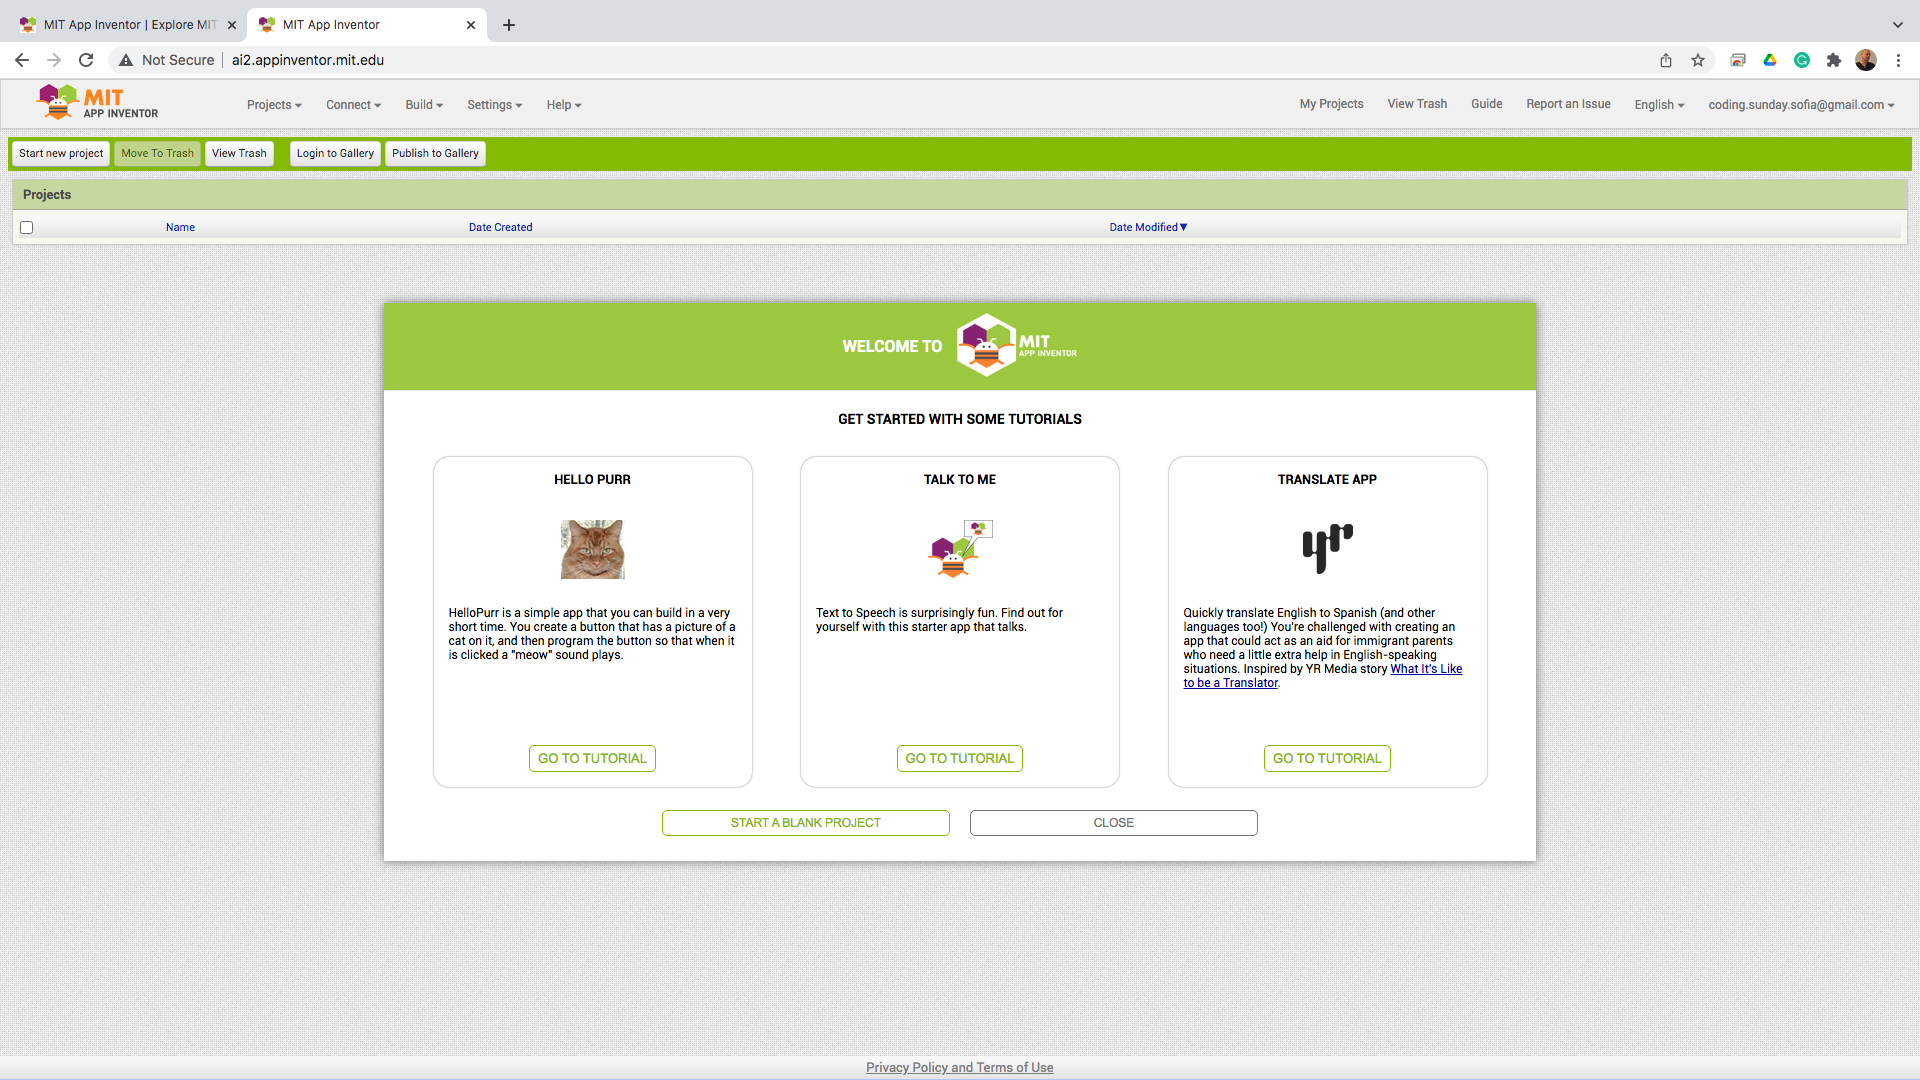
\includegraphics[width=1.0\linewidth,height=0.5\linewidth]{fig010026.png}
   \caption{Ability to choose learning projects}
\label{fig010026}
\end{figure}

If a user does not select a learning project or choose the option to create an empty project, the system will redirect them to a page displaying a list of their projects (Fig. \ref{fig010027}, which cannot be displayed in a text-based format). This page provides an overview of the projects the user has created and saved within their App Inventor account.

The list of projects serves as a central hub for users to manage and access their ongoing app development work. Each project is typically represented by a title or name, allowing users to quickly identify and select the project they wish to work on.

From this page, users can perform various actions related to their projects, such as opening a project for further editing, making copies of projects, or deleting no longer-needed projects. This centralized view helps users keep track of their progress, organize their work, and seamlessly navigate between different projects.

By displaying the list of their projects, App Inventor ensures that users have easy and convenient access to their previously created projects, enabling them to continue their app development journey from where they left off.

\begin{figure}[H]
   \centering
   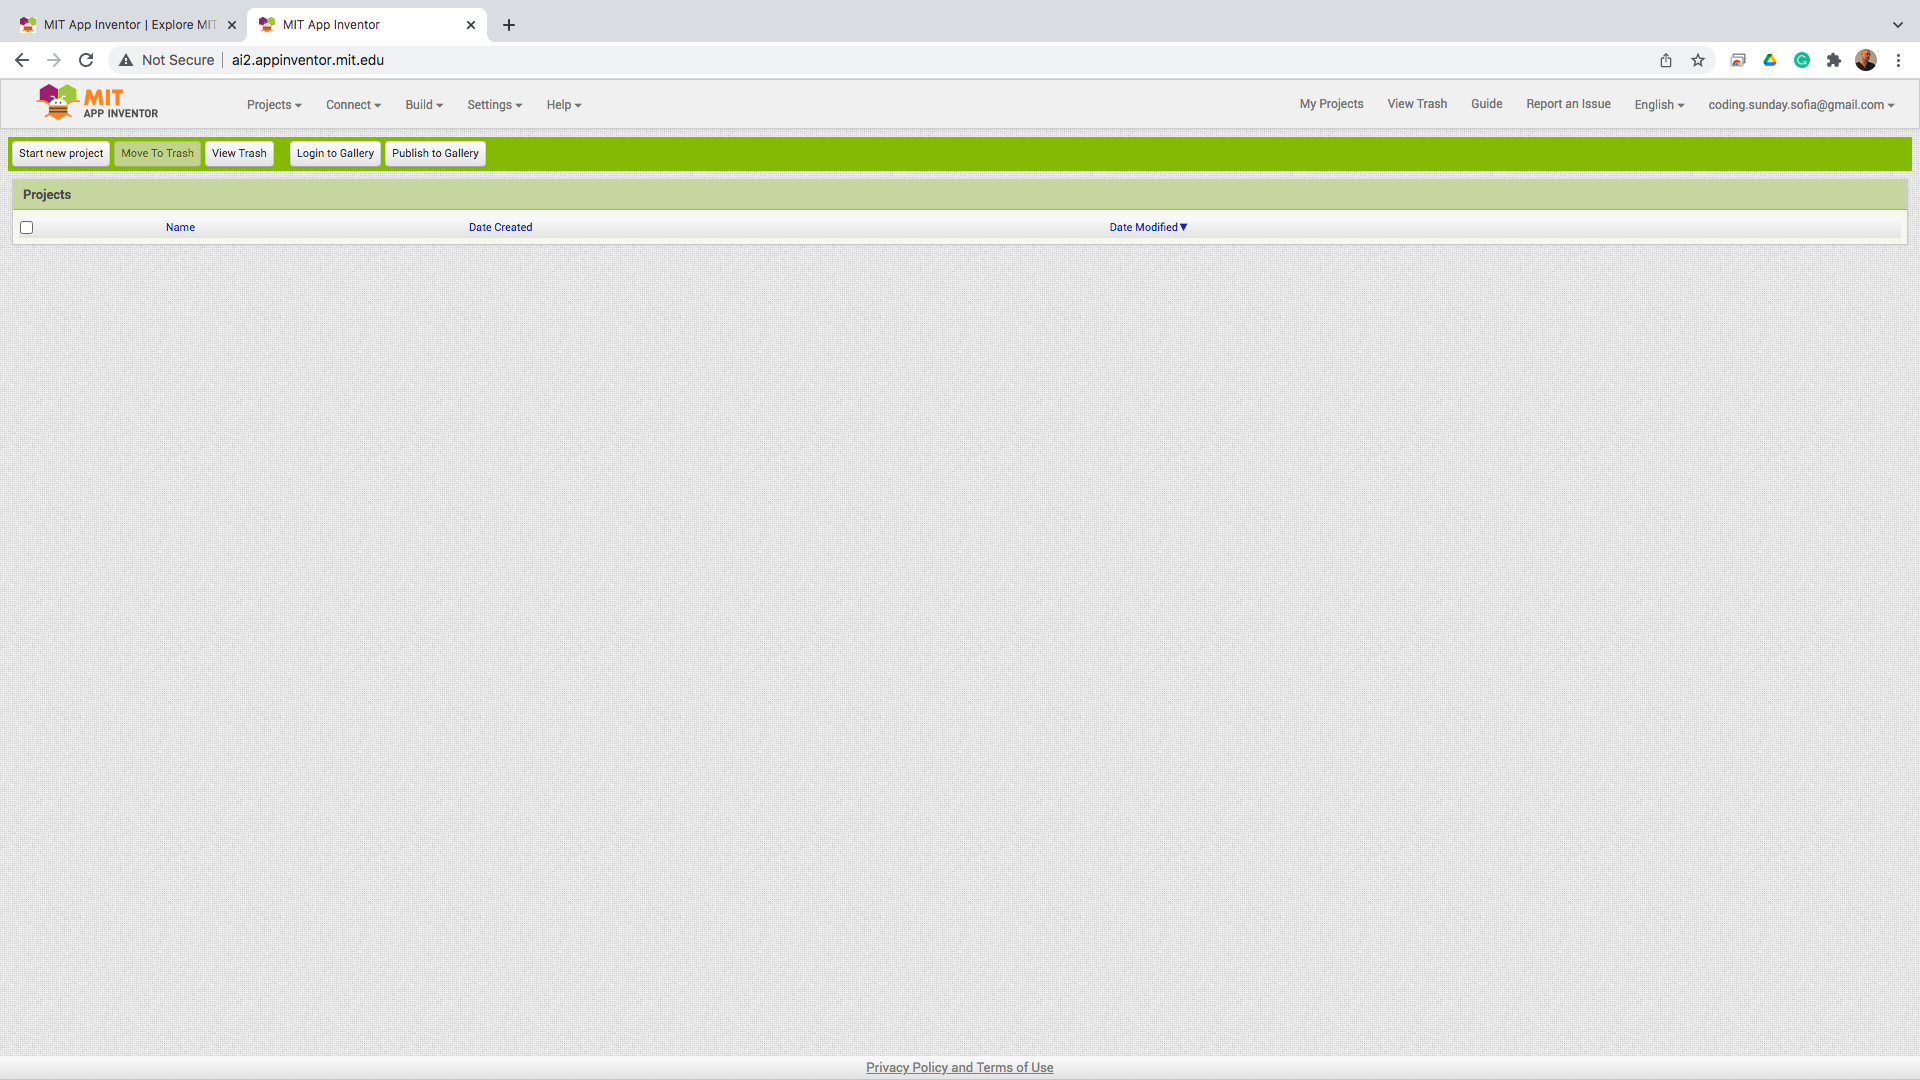
\includegraphics[width=1.0\linewidth,height=0.5\linewidth]{fig010027.png}
   \caption{Own Projects List Page}
\label{fig010027}
\end{figure}

To start a new project in the App Inventor programming environment, you can click on the "New Project" button located at the top left corner of the main work screen (Fig. \ref{fig010028}, which cannot be displayed in a text-based format). This button is a starting point for creating a new project and initiating your app development process.

By clicking on the "New Project" button, you will be prompted to provide a name for your new project. This name can be descriptive and should reflect the purpose or theme of your app. After entering the lovely name, you can create your project and work on your app's design and functionality.

Starting a new project gives you a blank canvas to unleash your creativity and develop your app from scratch. You can utilize various components, blocks, and features App Inventor offers to bring your app idea to life.

By providing an easily accessible "New Project" button, App Inventor ensures that users can swiftly start new projects and embark on their app development journey without any unnecessary hurdles or complications.

\begin{figure}[H]
   \centering
   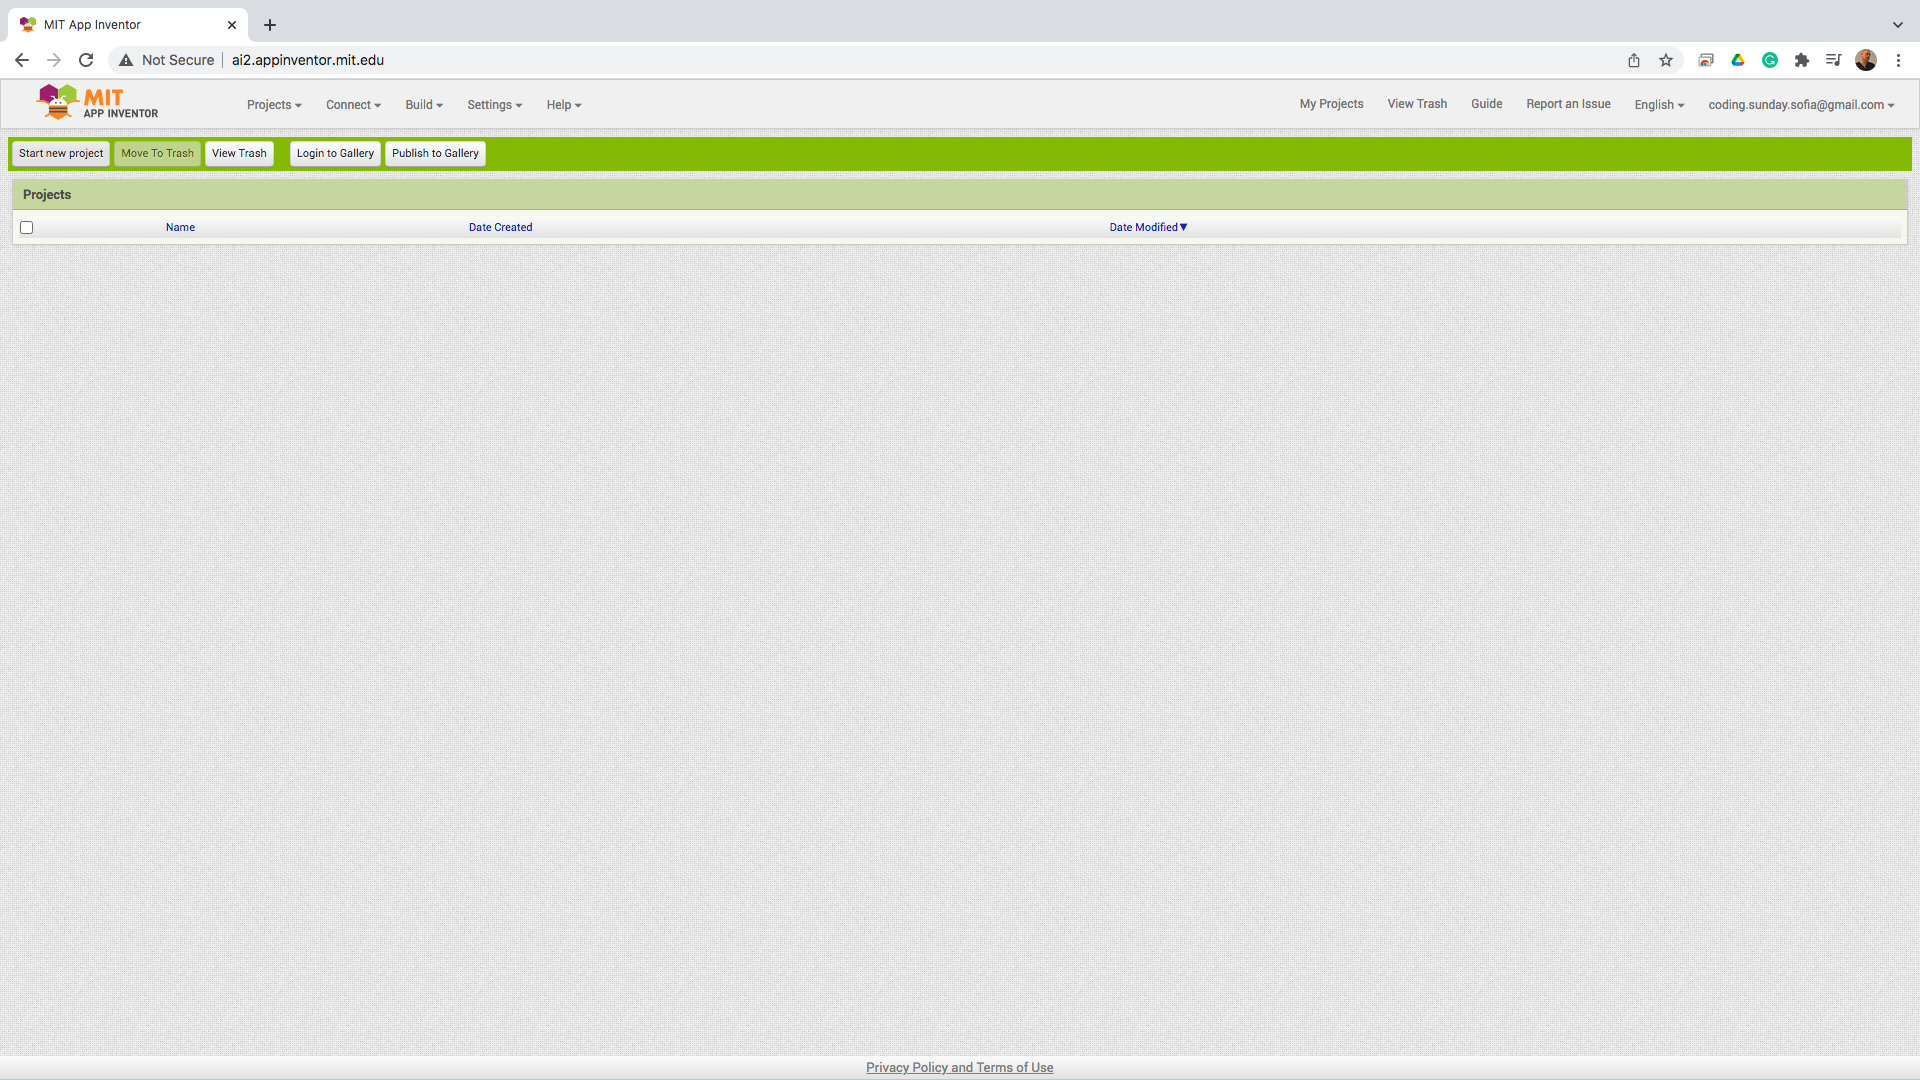
\includegraphics[width=1.0\linewidth,height=0.5\linewidth]{fig010028.png}
   \caption{Start New Project Button}
\label{fig010028}
\end{figure}

In the App Inventor programming environment, work is organized through projects, and each project is assigned an appropriate name when created (Fig. \ref{fig010029}, which cannot be displayed in a text-based format).

When creating a new project, one of the initial steps is to provide a name that accurately represents the purpose or theme of the project. This name helps you identify and distinguish your projects within the App Inventor environment, especially when multiple projects are in progress.

Choosing an appropriate name for your project is essential for effective organization and easy retrieval. It allows you to quickly locate and work on the specific project you desire, especially when you have an extensive collection of projects over time.

App Inventor facilitates a structured and organized approach to managing your app development endeavors by assigning a name to each project. It ensures that you can easily navigate your projects, stay focused on specific tasks, and maintain clarity and efficiency in your coding and development process.

\begin{figure}[H]
   \centering
   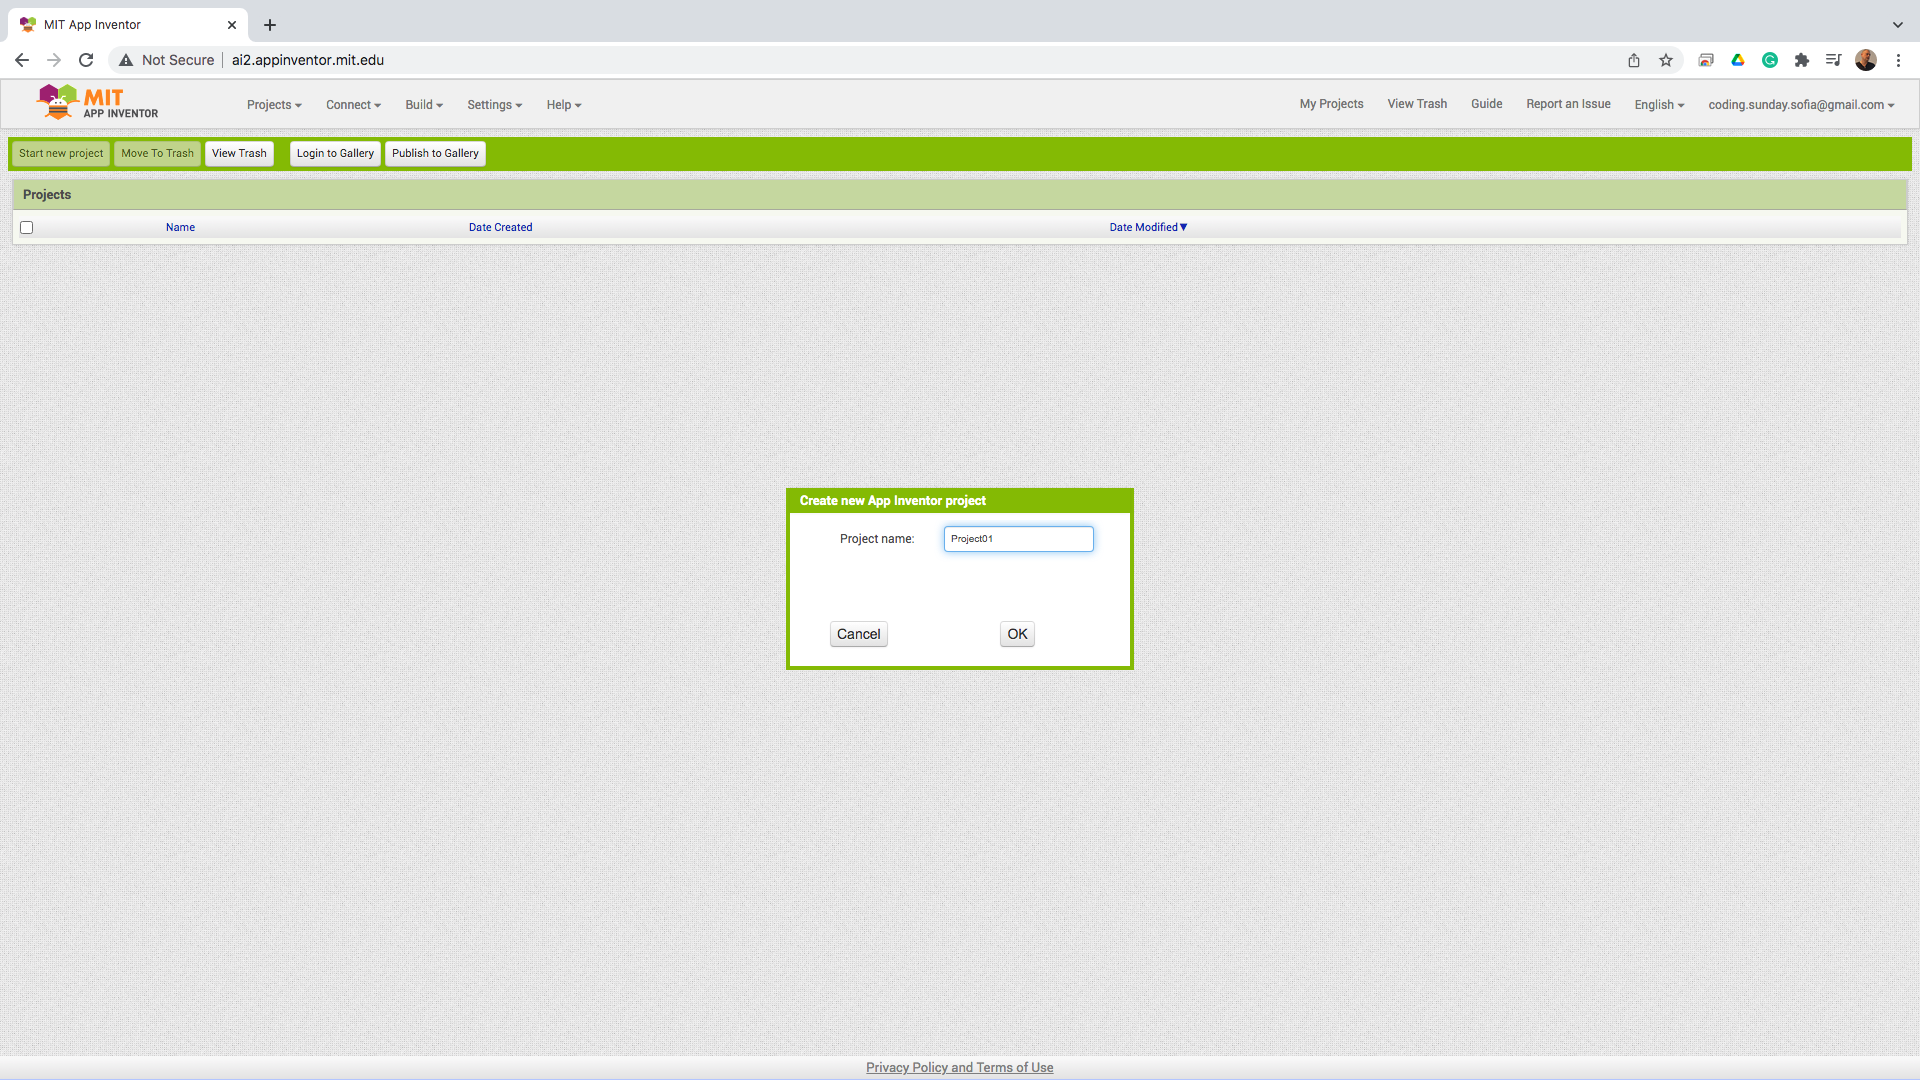
\includegraphics[width=1.0\linewidth,height=0.5\linewidth]{fig010029.png}
   \caption{Project Name}
\label{fig010029}
\end{figure}

After selecting a name for your project in the App Inventor programming environment, the interface visualizes the first working screen, providing you with the opportunity to design the visual user interface (Fig. \ref{fig010030}, which cannot be displayed in a text-based format). Creating the graphical user interface involves dragging and dropping various visual controls into the main work area.

The visual controls represent different elements that users interact with in your app, such as buttons, labels, text boxes, images, and more. These controls are available in the palette or toolbox, typically on the screen's left side. Selecting a control and dragging it onto the main work area allows you to position and arrange it as desired.

This drag-and-drop approach allows you to design the layout and appearance of your app's user interface. You can visually organize the controls, resize and customize them, and create an intuitive and engaging user experience.

App Inventor simplifies designing the visual user interface by eliminating the need for complex coding. Instead, it emphasizes a visual and intuitive approach, allowing you to focus on the design aspects of your app without getting overwhelmed by technical details.

By providing a user-friendly interface and a drag-and-drop feature for visual control placement, App Inventor empowers users to create appealing and functional user interfaces for their mobile applications.

\begin{figure}[H]
   \centering
   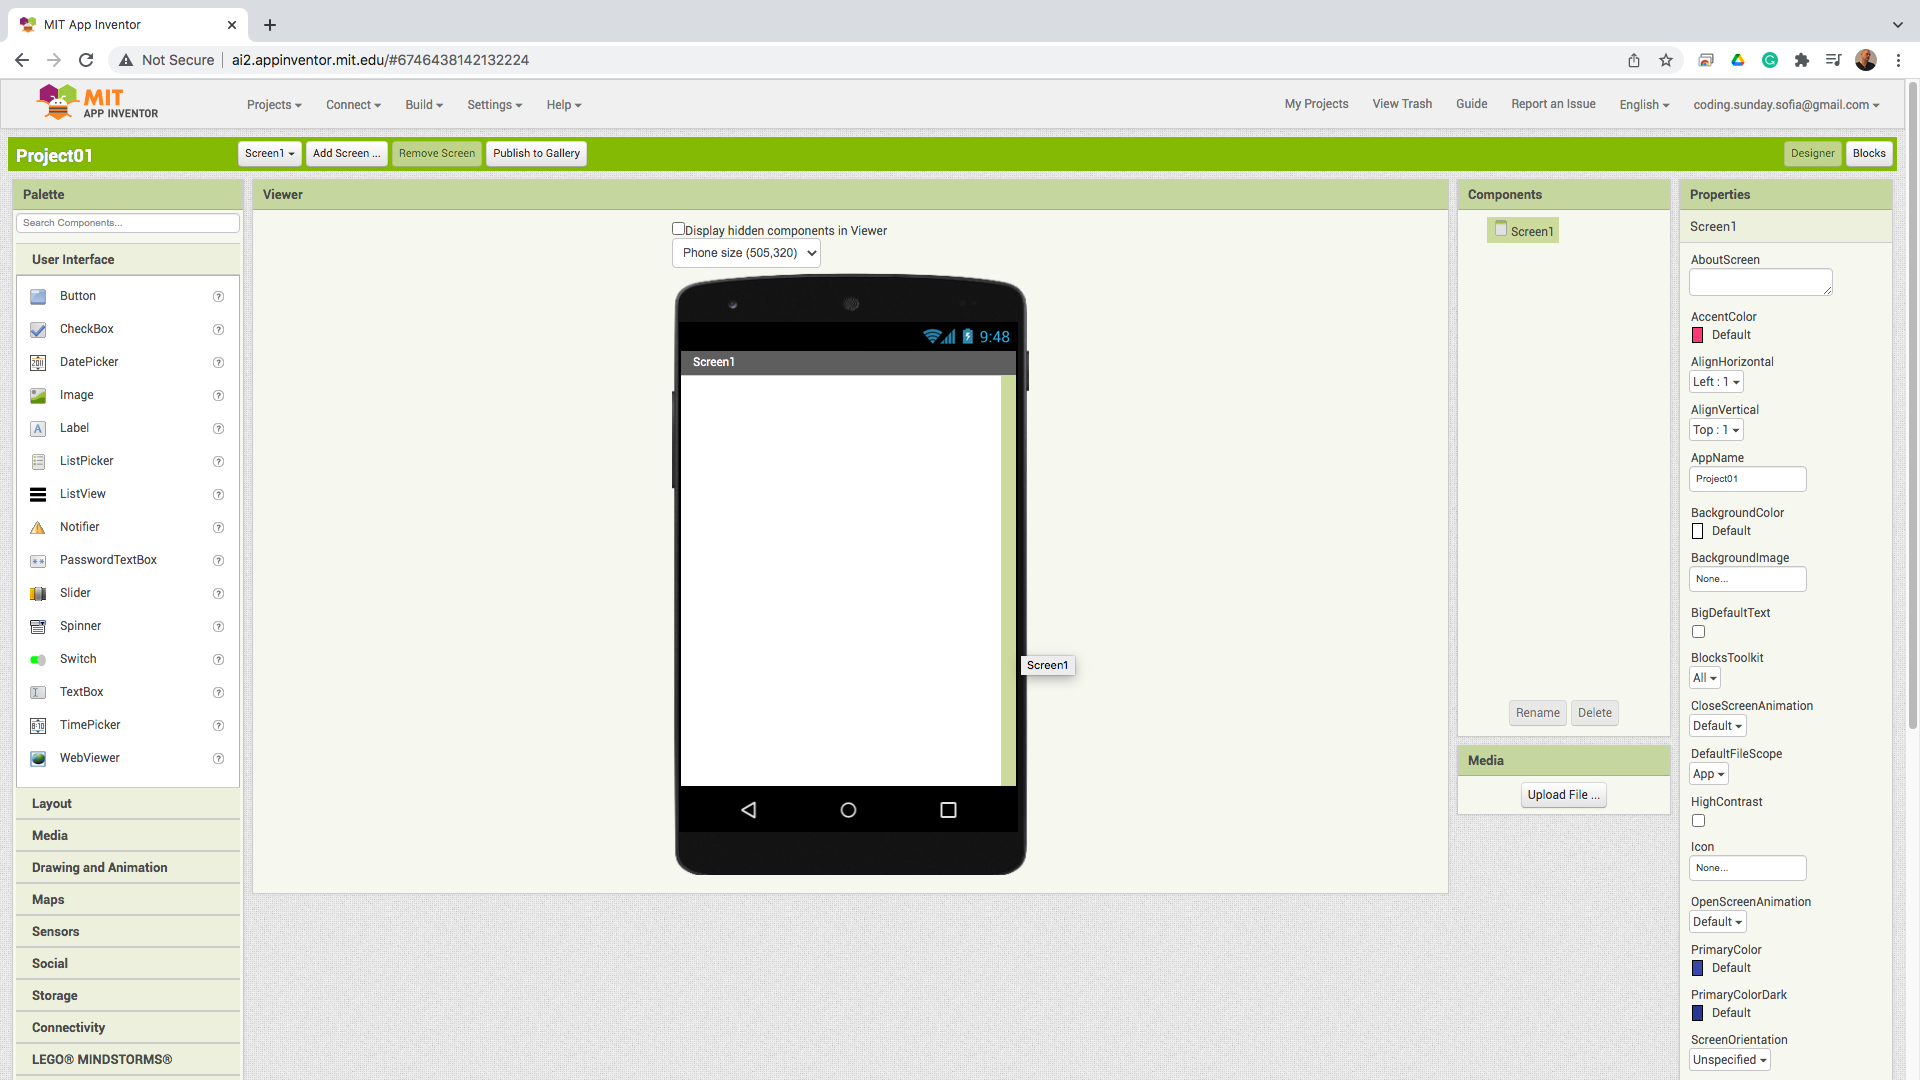
\includegraphics[width=1.0\linewidth,height=0.5\linewidth]{fig010030.png}
   \caption{Design view of the development environment}
\label{fig010030}
\end{figure}

In the App Inventor programming environment, the button is one of the primary visual controls available. The button represents a designated area in the visual field that typically has a text label or icon to visually represent an action performed when the button is pressed (Fig. \ref{fig010031}, which cannot be displayed in a text-based format).

The button control is an interactive element in your app's user interface, allowing users to trigger specific actions or events. Adding a button to your app's design provides a clear and intuitive way for users to initiate functionality or navigate through different sections of your app.

You can use a button control to demonstrate the process of working with the compiled program code. You can customize the button's appearance by setting its properties, such as the text label, color, size, and position on the screen. Additionally, you can define the specific behavior of the button by assigning event handlers or programming logic to execute when the button is pressed.

Utilizing the button control in your app's design allows you to create interactive and responsive user interfaces that enhance user engagement and provide a seamless user experience. The button serves as a bridge between the visual design of your app and the functional logic implemented through programming code, allowing users to interact with your app and easily trigger desired actions.

\begin{figure}[H]
   \centering
   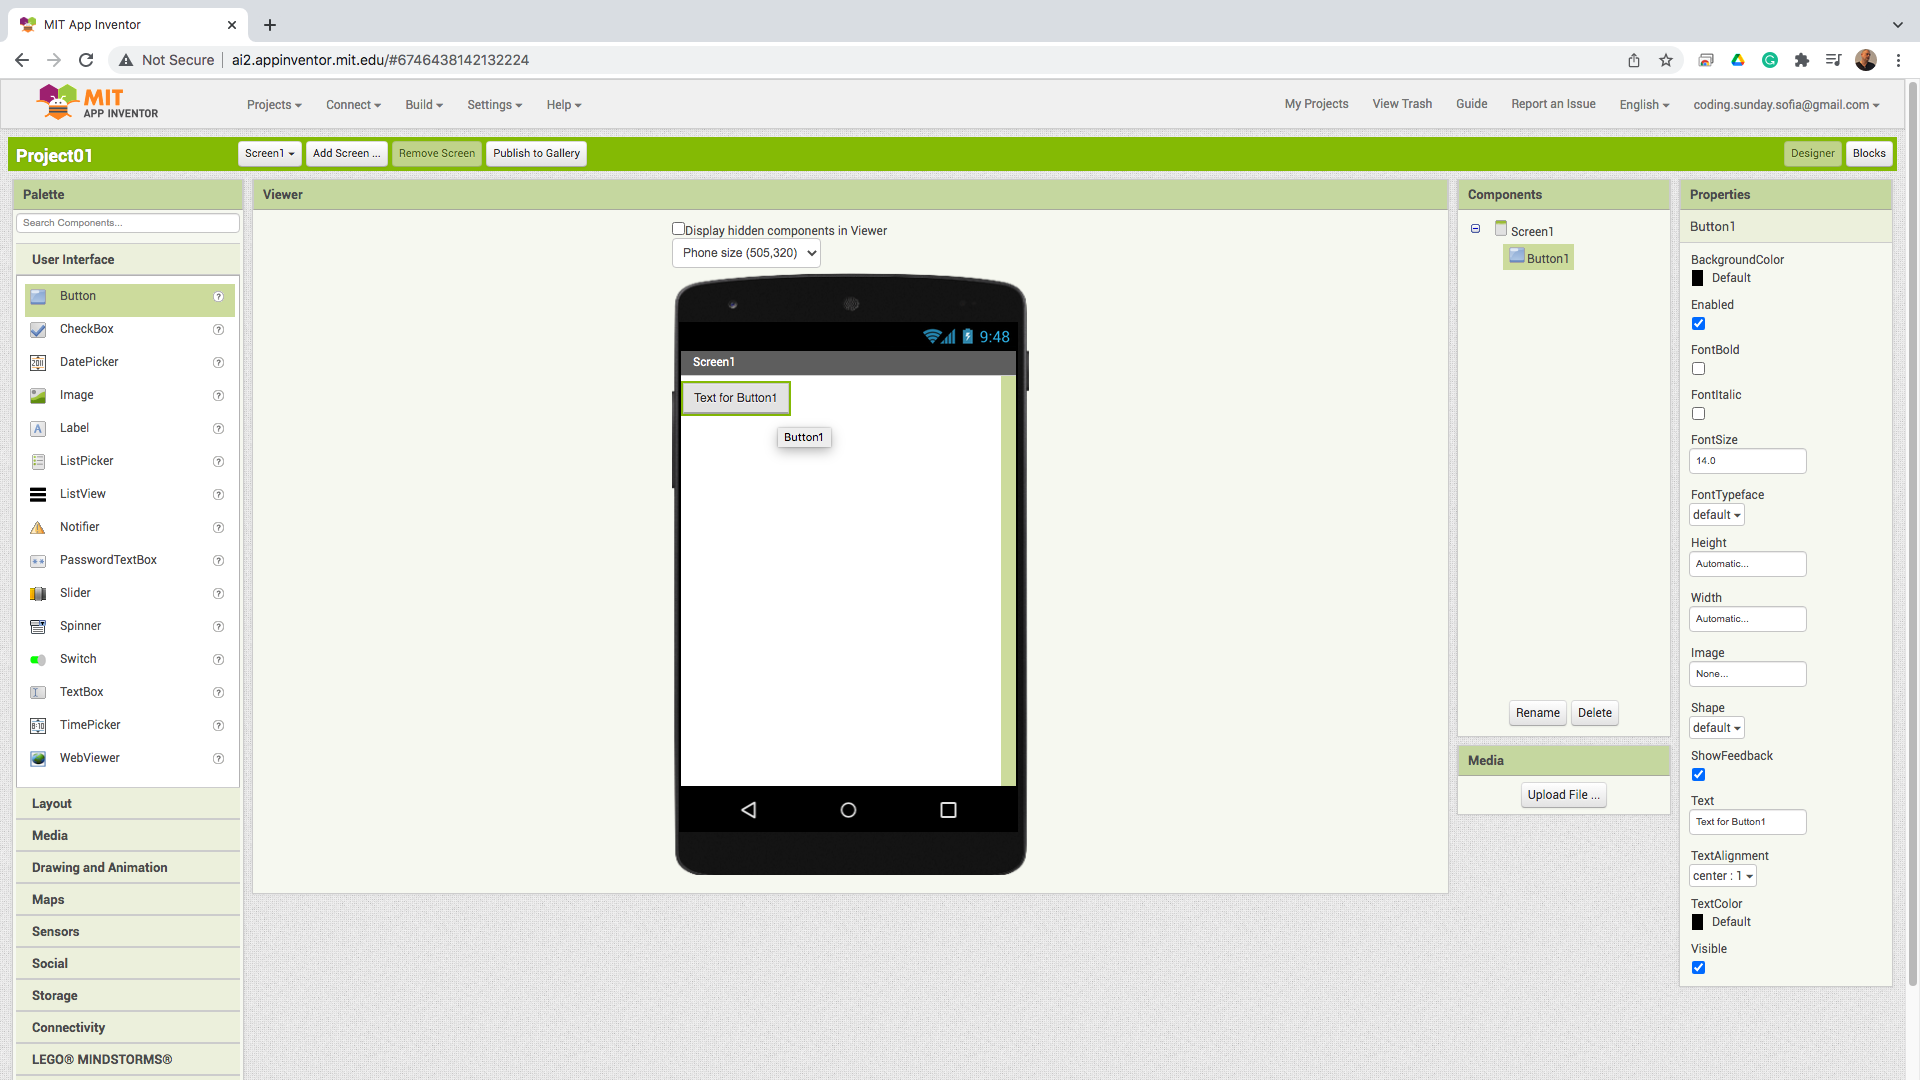
\includegraphics[width=1.0\linewidth,height=0.5\linewidth]{fig010031.png}
   \caption{Place button}
\label{fig010031}
\end{figure}

When designing software applications, using expressive and meaningful names for buttons and other interactive elements is crucial. These names should convey the intended action or functionality to the users. In the case of the button in question (Fig. \ref{fig010031}, which cannot be displayed in a text-based format), the name "Push" is used.

The name "Push" suggests a straightforward and intuitive action to the users, indicating that pressing the button will initiate a specific action or behavior. By choosing a concise and descriptive name like "Push," users can quickly understand the button's purpose and anticipate the outcome of pressing it.

Using expressive names for buttons enhances your software application's usability and user experience. It helps users navigate and interact with the interface more effectively, reducing confusion and improving the overall accessibility of your app. By providing clear and meaningful button names, you enable users to intuitively engage with your application's functionality, enhancing their satisfaction and engagement.

\begin{figure}[H]
   \centering
   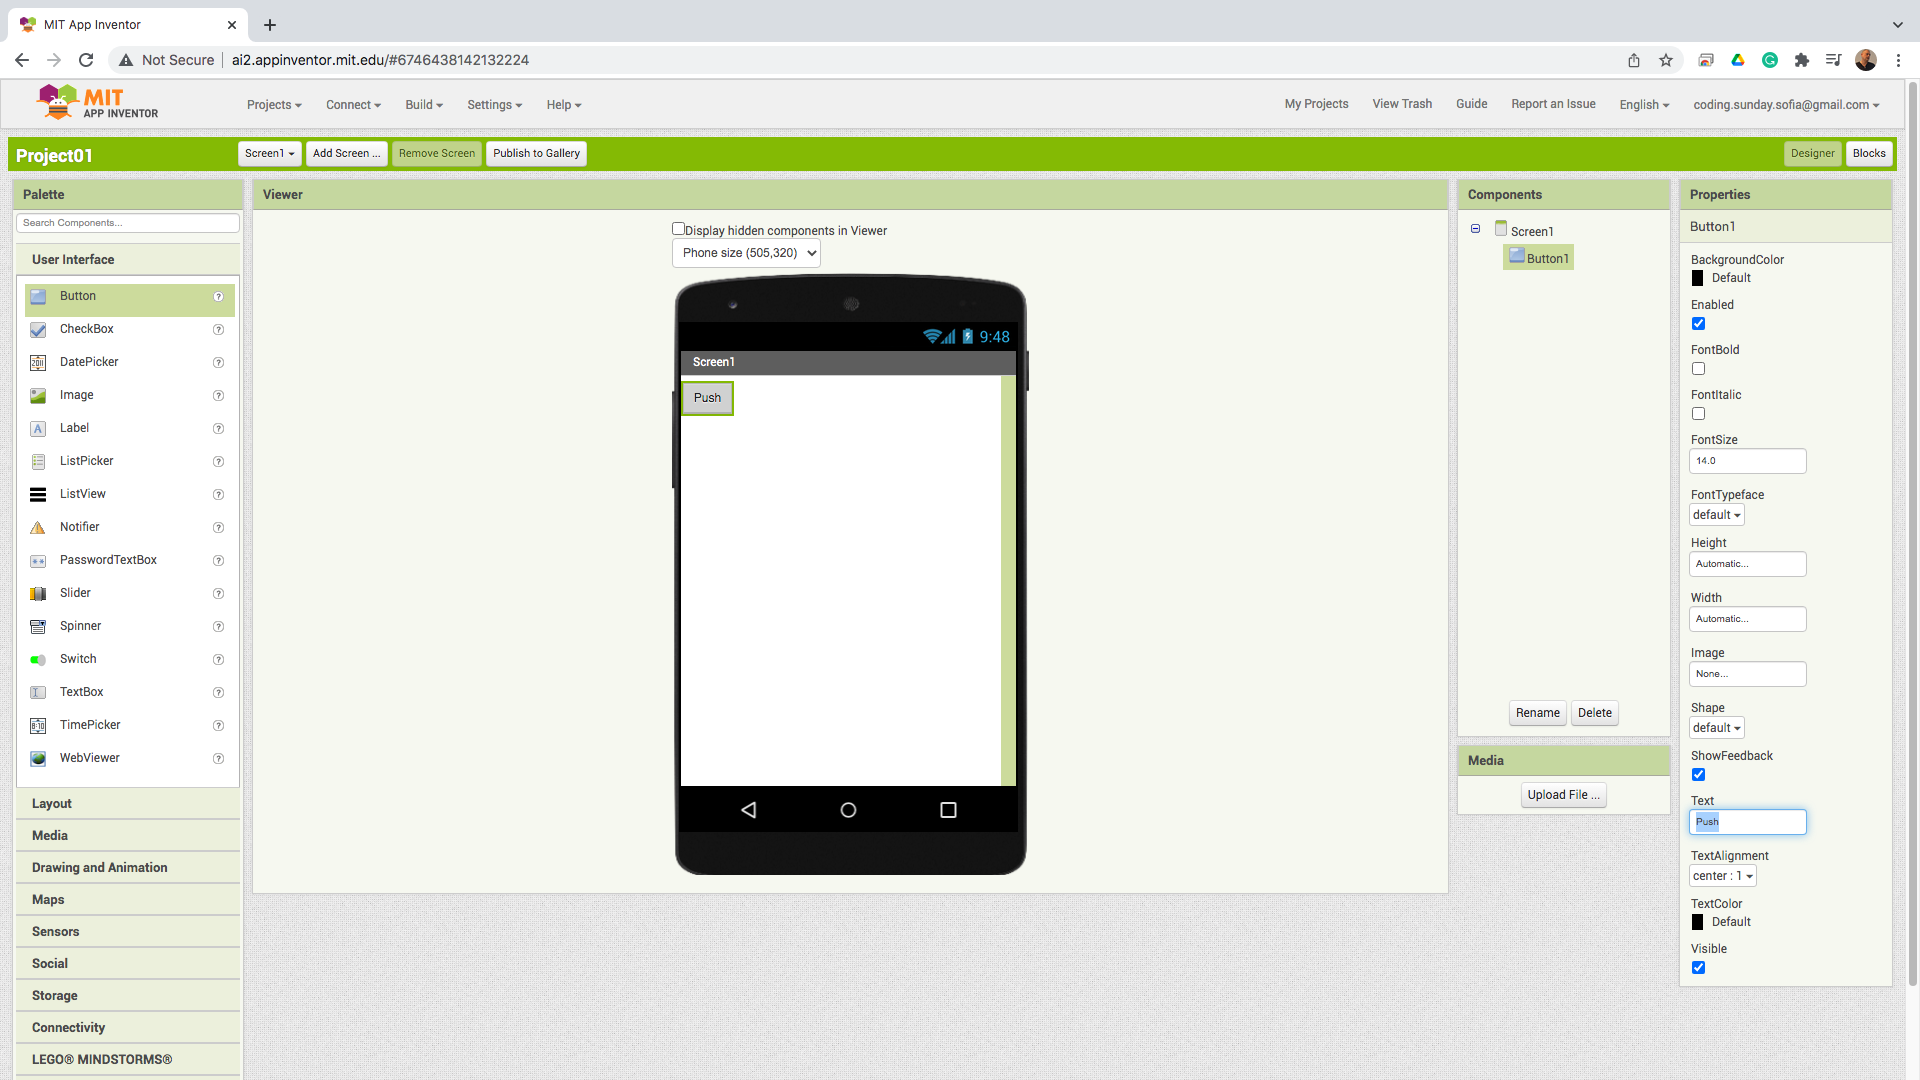
\includegraphics[width=1.0\linewidth,height=0.5\linewidth]{fig010032.png}
   \caption{Select text on button}
\label{fig010032}
\end{figure}

Unlike the Scratch programming environment where program instructions are represented as blocks directly in the main workspace, in App Inventor, the program instructions are organized in a separate work screen known as the "Blocks Editor" (Fig. \ref{fig010033}, which cannot be displayed in a text-based format).

The Blocks Editor in App Inventor provides a dedicated space for assembling the program instructions in a puzzle-like format. It allows users to connect visually and arrange blocks representing different programming logic and actions. Each block corresponds to a specific function or operation that can be performed within the app.

By separating the program instructions into the Blocks Editor, App Inventor aims to provide a more organized and structured approach to programming. Users can quickly locate and manipulate the desired blocks, connecting them to define the behavior and functionality of their app. The puzzle-like arrangement of the blocks fosters a logical and intuitive understanding of the code flow and structure.

Users can explore blocks corresponding to different programming concepts in the Blocks Editor, such as control structures, event handlers, data manipulation, and more. Users can build complex program logic without writing traditional text-based code by dragging and connecting the blocks.

The separation of program instructions into the Blocks Editor allows users to focus on the visual representation and arrangement of the code, making it accessible and engaging for beginners and those who prefer a more visual approach to programming. It provides a unique way to construct programs, promoting creativity and problem-solving skills.

\begin{figure}[H]
   \centering
   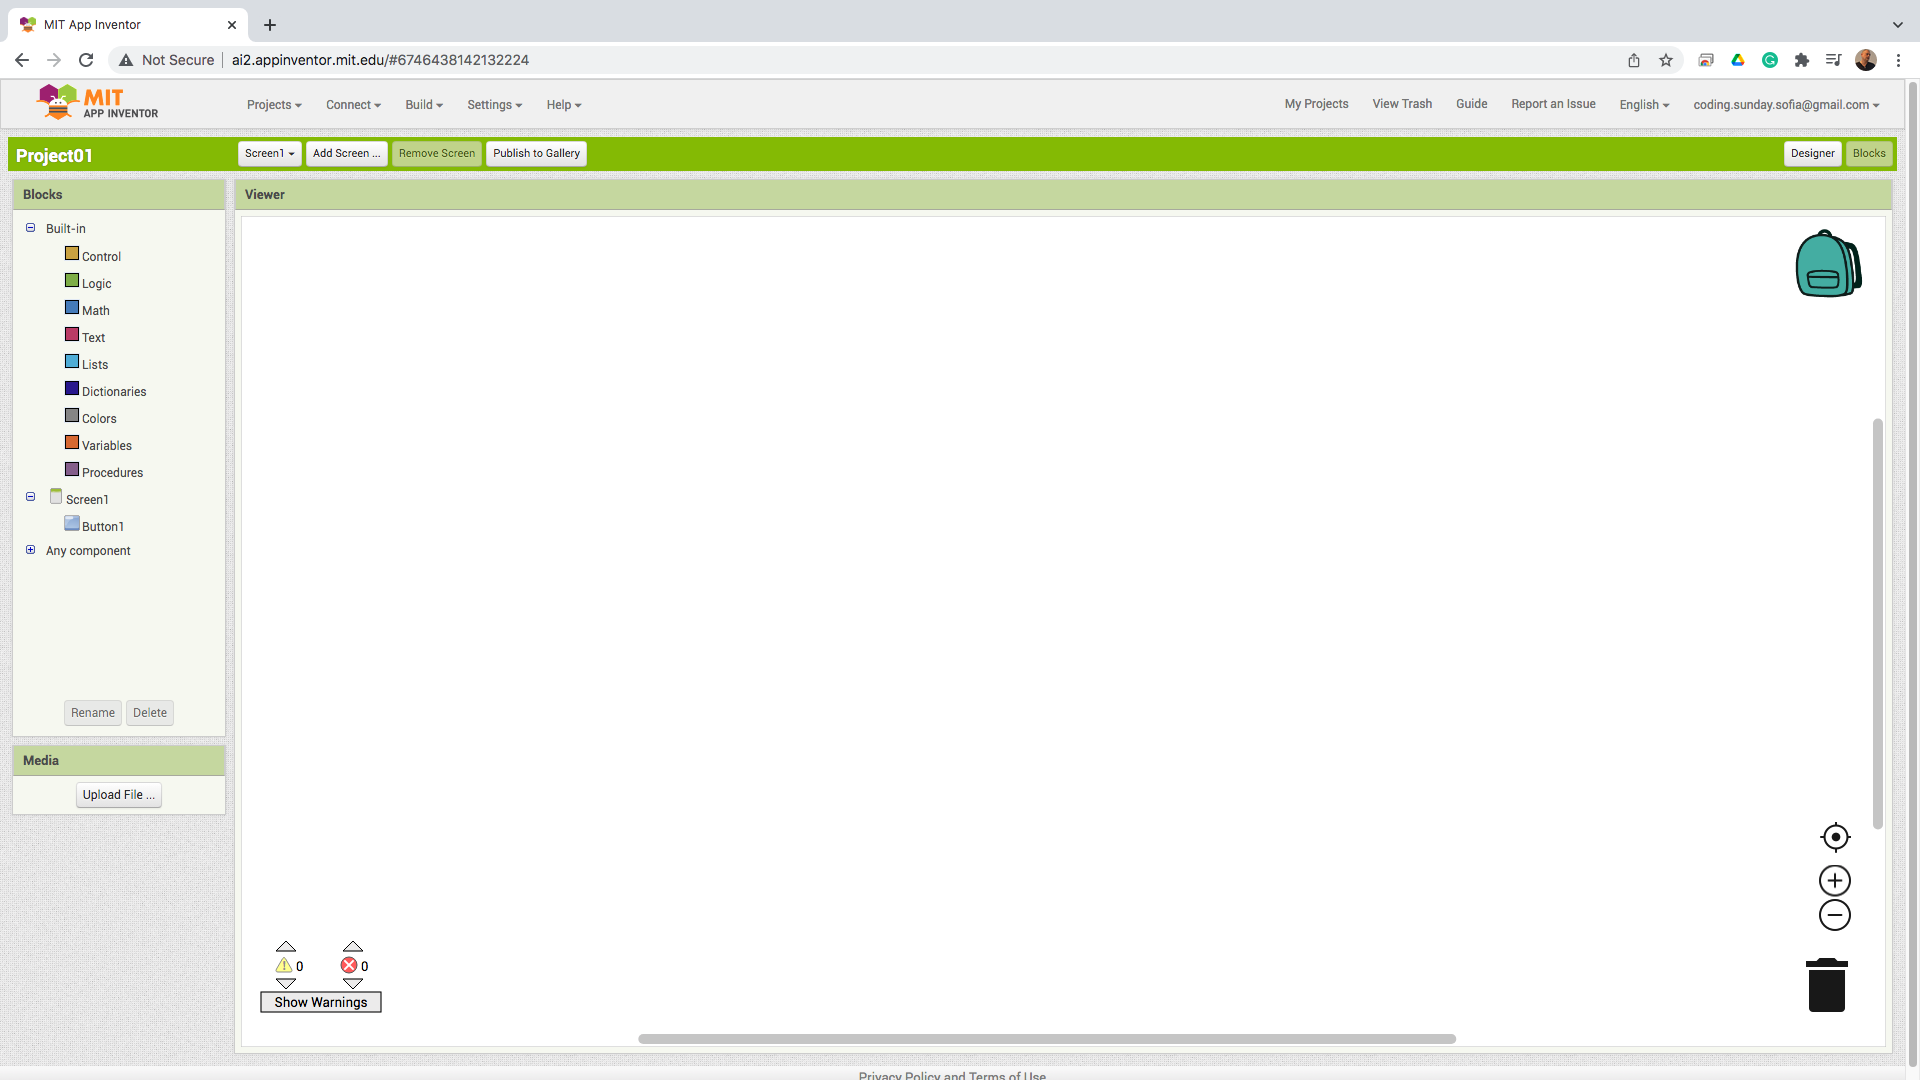
\includegraphics[width=1.0\linewidth,height=0.5\linewidth]{fig010033.png}
   \caption{Program view of the development environment}
\label{fig010033}
\end{figure}

In App Inventor, the execution of program instructions is based on event-driven programming. Instead of having a predefined starting point and endpoint like in Scratch, App Inventor programs respond to specific events triggered by user interactions or other system events.

When the program is run in App Inventor, it first visualizes the graphical user interface (GUI) components designed in the workspace. The program then waits for specific events, such as a button click, screen touch, sensor input, or timer expiration.

In the example shown in Fig. \ref{fig010034} (which cannot be displayed in a text-based format), the program is waiting for the user to interact with the "Push" button. Once the user clicks the button, the associated event is triggered, and the program executes the instructions connected to that event.

App Inventor uses event handlers to define the actions that should occur when a specific event is triggered. These event handlers are represented as blocks in the Blocks Editor and are associated with the corresponding graphical components on the GUI.

App Inventor allows users to create interactive and responsive apps by leveraging events. The program instructions associated with each event can include various actions, such as displaying messages, performing calculations, updating the interface, or even interacting with external services and APIs.

The event-driven approach in App Inventor provides a flexible and intuitive way to design apps that respond to user input and external stimuli. It allows for creating dynamic and interactive experiences, empowering users to build functional and engaging mobile applications without the need for extensive coding knowledge.

\begin{figure}[H]
   \centering
   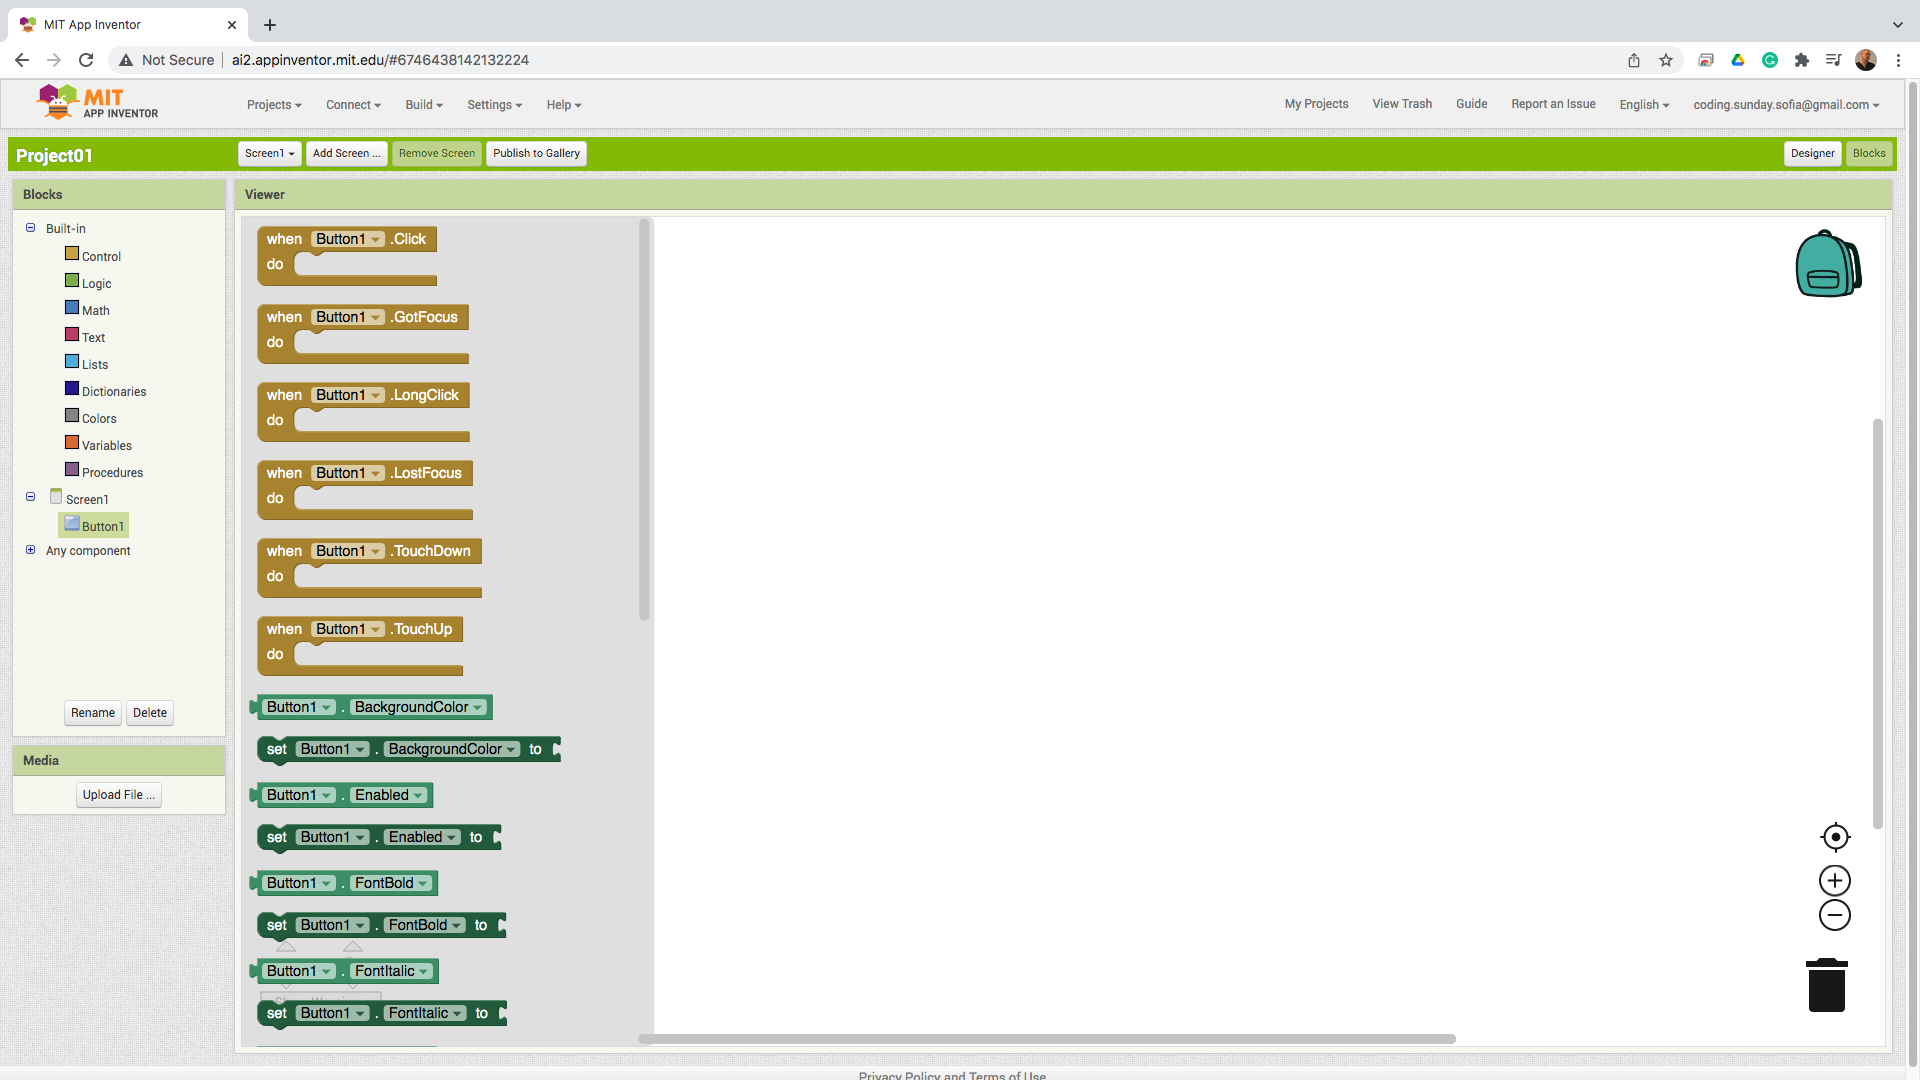
\includegraphics[width=1.0\linewidth,height=0.5\linewidth]{fig010034.png}
   \caption{List of instructions}
\label{fig010034}
\end{figure}

In App Inventor, the button component generates an event called "Click" when pressed. This event can be captured in the Blocks Editor, where specific actions can be defined to execute when the button clicks.

In Fig. \ref{fig010035}, the Blocks Editor shows the event handler for the "Click" event of the button component. When the button clicks, the program will execute the instructions connected to this event handler.

In this example, the event handler consists of a single instruction represented by the "Say Hello World" block. This block is a text-to-speech component that will speak the phrase "Hello World" when the button is clicked.

The event handler in the Blocks Editor allows you to add more instructions or blocks to perform various actions in response to the button click event. These actions can include displaying messages, changing the appearance of other components, performing calculations, or even connecting to external services and APIs.

Users can create interactive behavior in their apps by associating specific actions with the button click event. The event-driven nature of App Inventor allows for creating dynamic and responsive applications without the need for complex programming syntax.

Overall, the event-handling feature in App Inventor provides a straightforward and intuitive way to define actions that should occur when specific events, such as button clicks, happen in the app.

\begin{figure}[H]
   \centering
   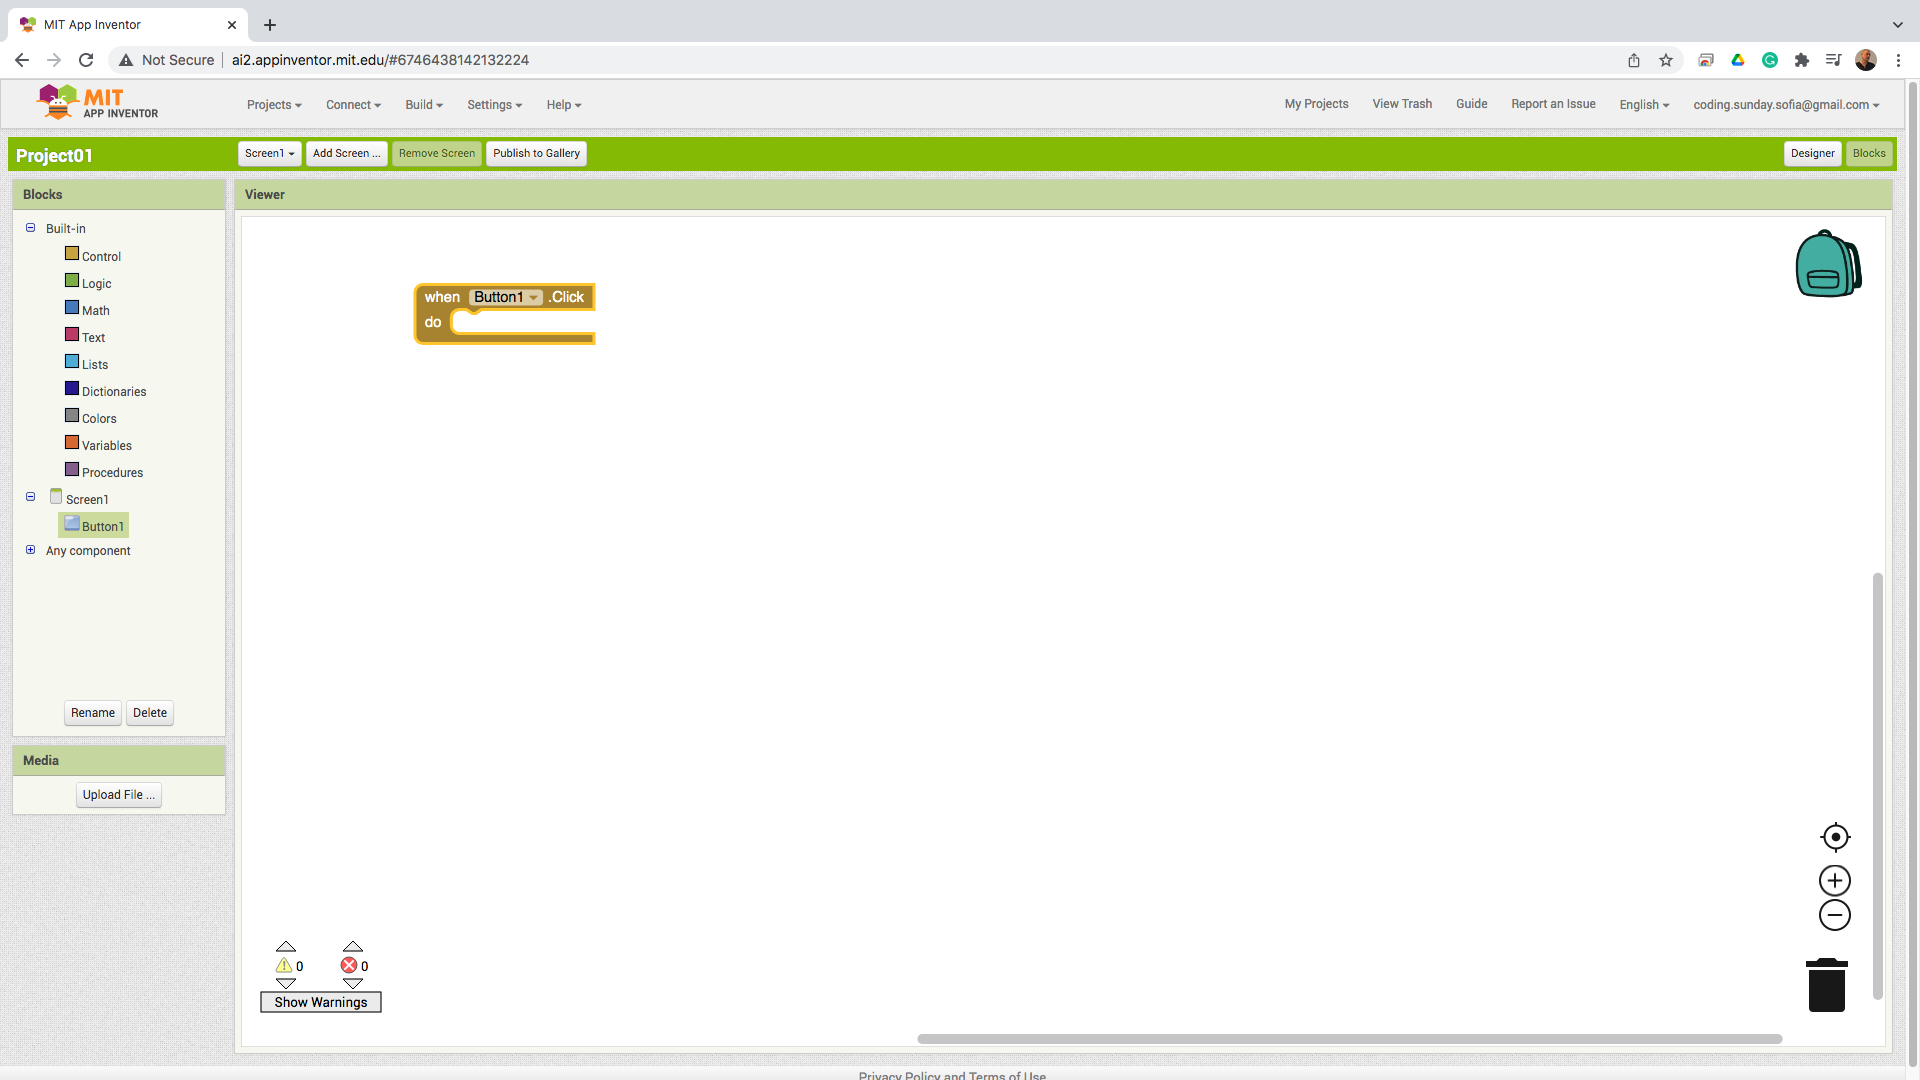
\includegraphics[width=1.0\linewidth,height=0.5\linewidth]{fig010035.png}
   \caption{Select event for button press}
\label{fig010035}
\end{figure}

The button press event in App Inventor is represented as a puzzle piece, commonly known as an event handler block. This block features a slot where you can insert the instructions to execute when the button is pressed (Fig. \ref{fig010036}).

The event handler block has a distinctive rounded shape and is labeled with the specific event it represents, such as "Button1.Click" indicating the click event of Button1 component. Within the event handler block, you can place additional blocks to define the actions or behaviors triggered by the button press.

By arranging the blocks inside the event handler, you have complete control over the flow and logic of your program. This visual representation simplifies creating event-driven programs and allows users, including beginners, to connect user interface components with desired actions easily.

The puzzle-like nature of App Inventor's event handler blocks makes it intuitive and engaging in building interactive behaviors in your applications without the need for complex coding syntax. It encourages creativity and empowers users to craft dynamic and responsive apps.

\begin{figure}[H]
   \centering
   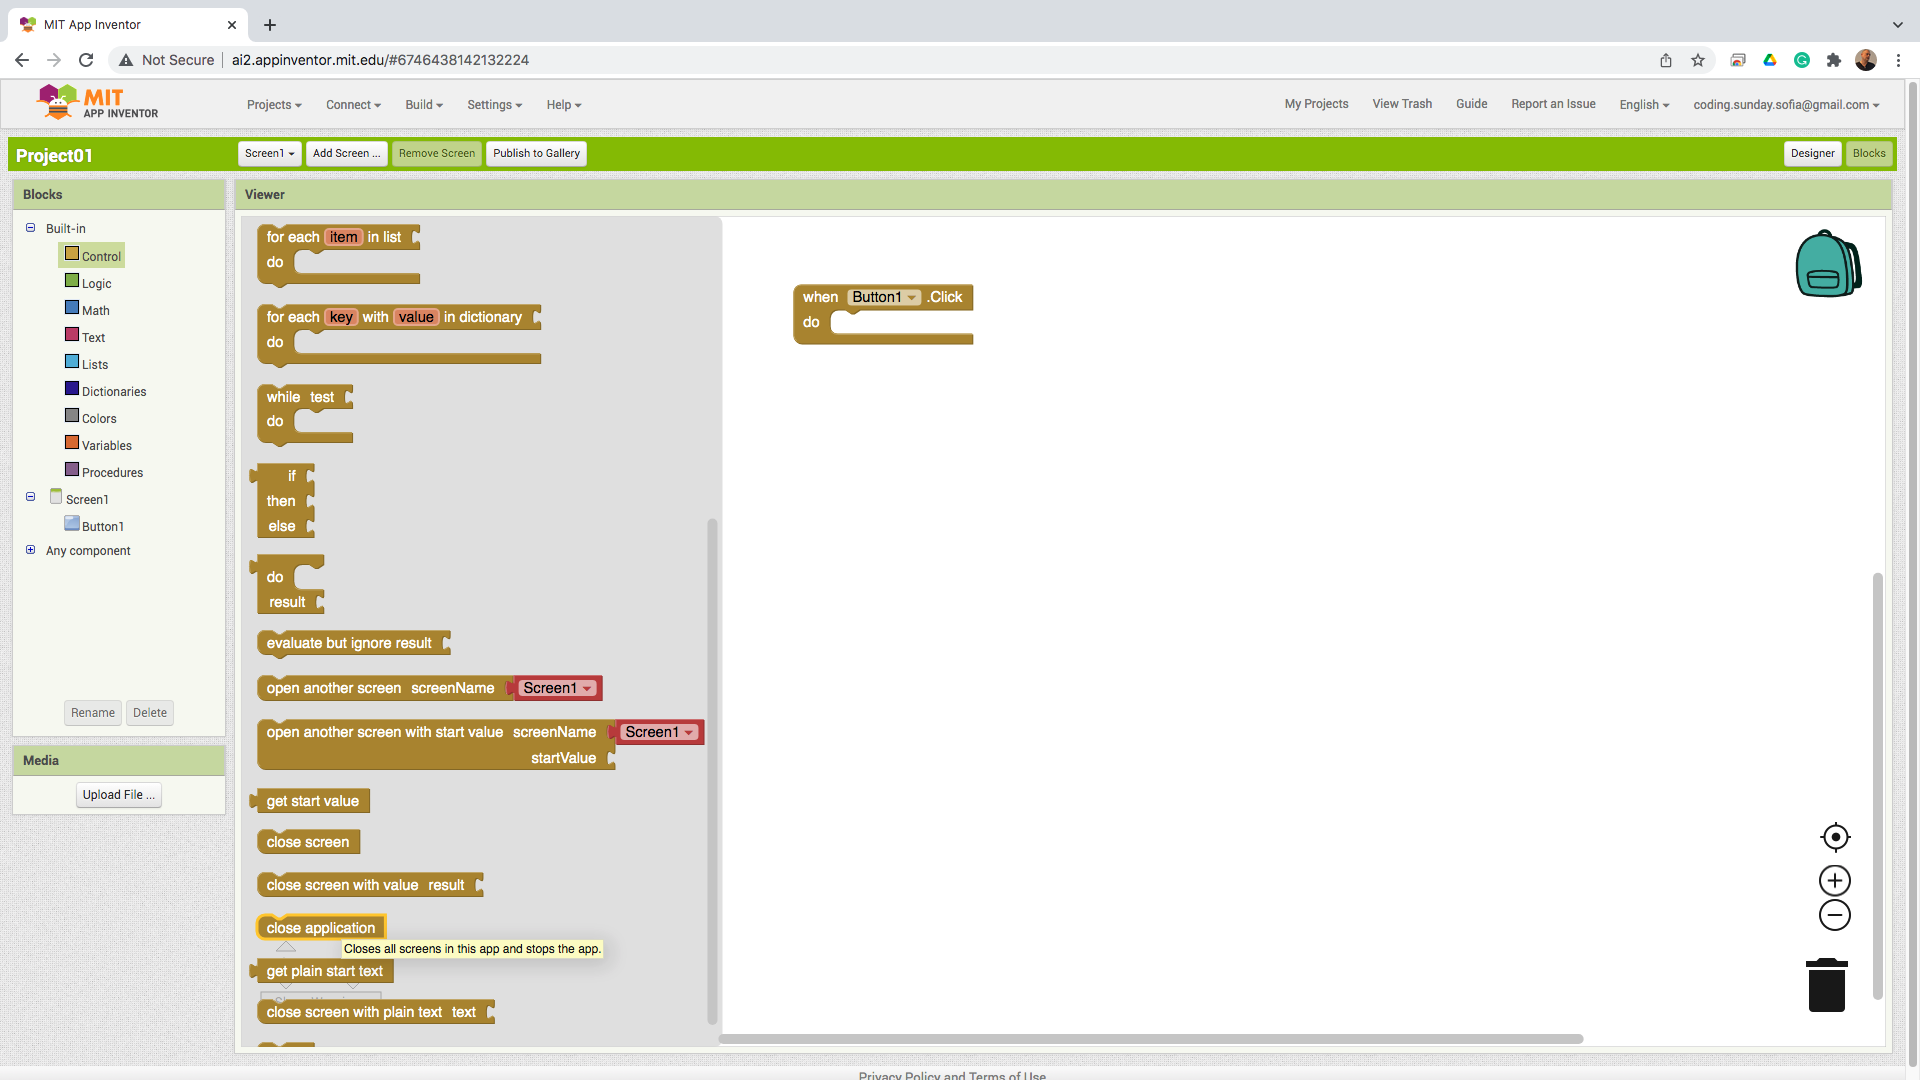
\includegraphics[width=1.0\linewidth,height=0.5\linewidth]{fig010036.png}
   \caption{Select action when button is pressed}
\label{fig010036}
\end{figure}

One of the most straightforward actions triggered by pressing the button is to stop the program and close the application window (Fig. \ref{fig010037}).

In App Inventor, this action is achieved using the "CloseScreen" block, a built-in instruction specifically designed to terminate the program and close the current window. When placed inside the event handler block for the button press event, the "CloseScreen" block will be executed as soon as the button is pressed.

The "CloseScreen" block ensures a smooth and controlled application termination, allowing users to exit the program effortlessly. This functionality is handy when creating simple applications or prototypes where a single button press can signify the end of the program's execution.

By utilizing the visual programming interface of App Inventor, even beginners can easily incorporate this action into their applications without the need for extensive coding knowledge. The simplicity and intuitiveness of App Inventor's block-based system empower users to quickly implement desired functionalities, enhancing the overall user experience of their applications.

\begin{figure}[H]
   \centering
   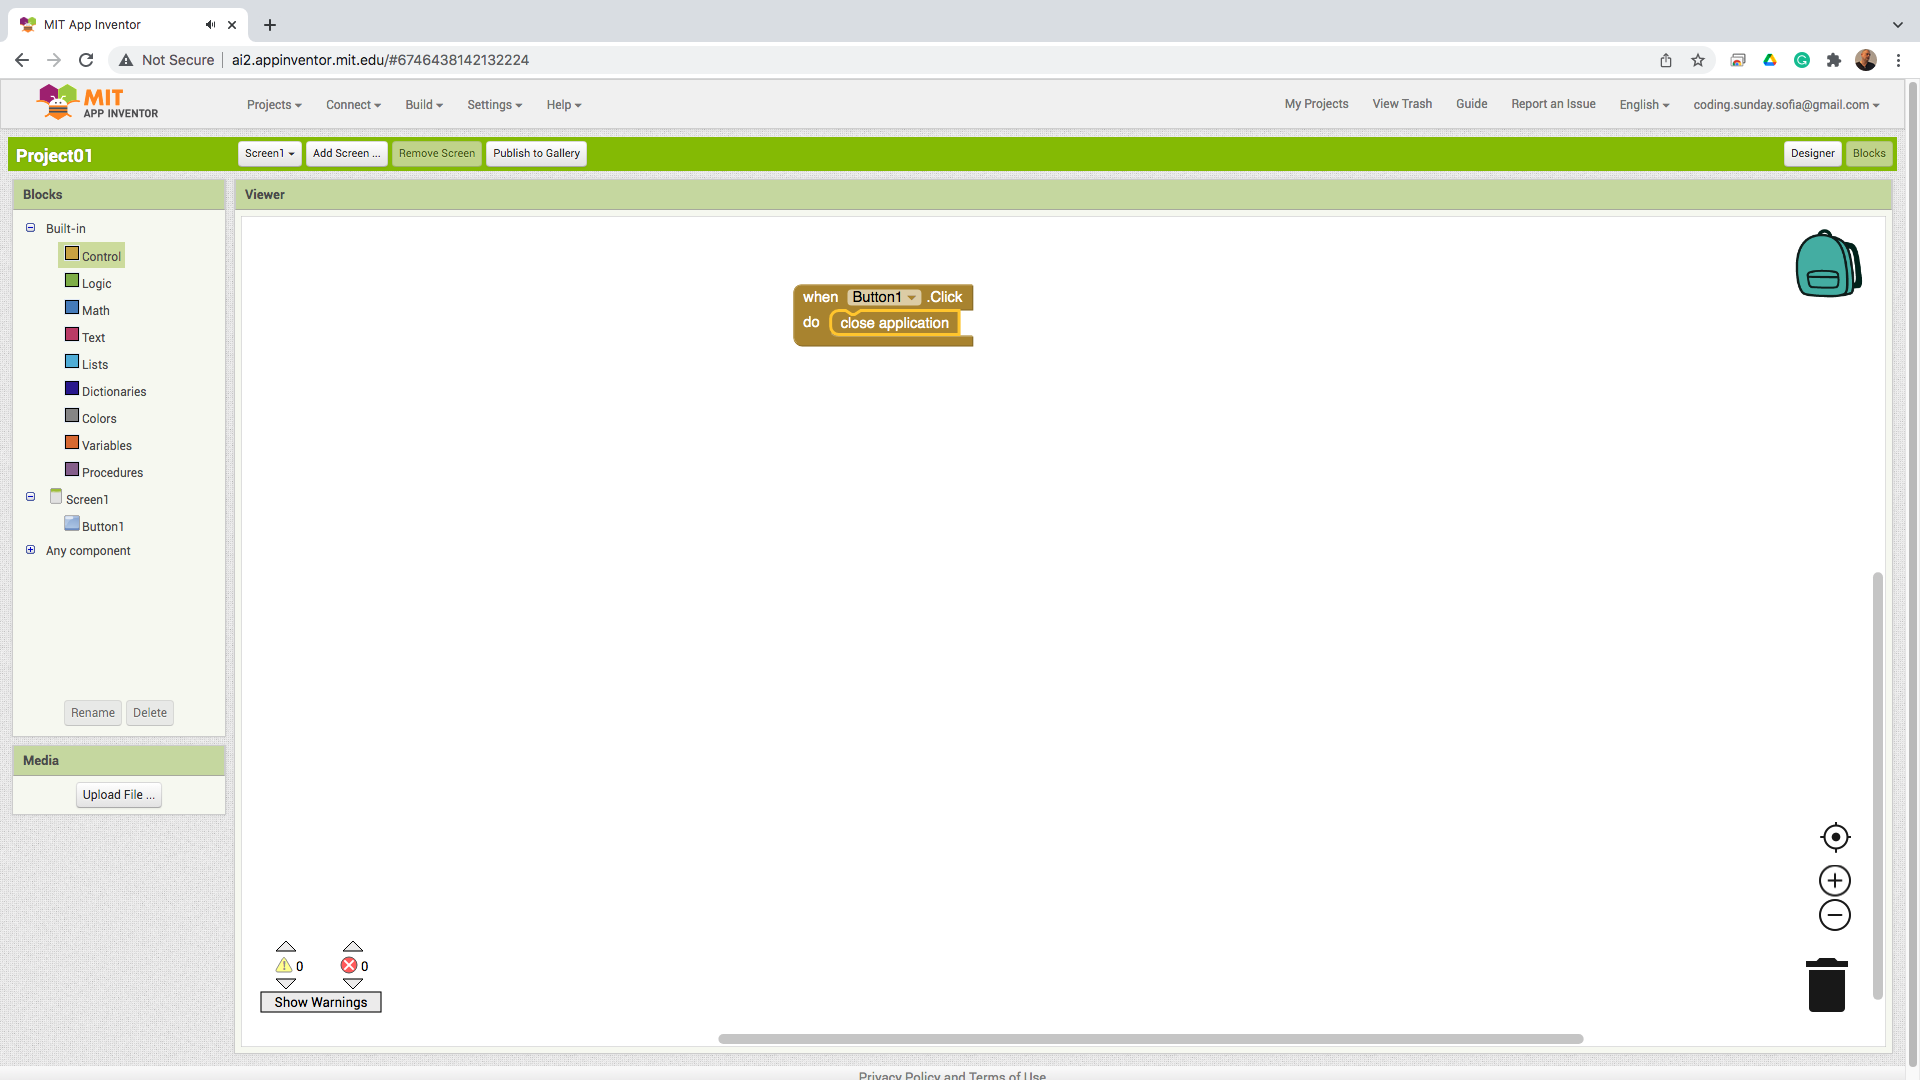
\includegraphics[width=1.0\linewidth,height=0.5\linewidth]{fig010037.png}
   \caption{Close application on button click}
\label{fig010037}
\end{figure}

Once the graphical programming interface is designed and the desired instructions are arranged, the next step is compiling the code and generating the complete program installation package (Fig. \ref{fig010038}).

In App Inventor, the compilation process takes the visual blocks and translates them into the corresponding code that the target device can execute. This includes converting the event handlers, such as button presses, into the necessary programming constructs and handling other program logic.

The compilation process ensures that the program is transformed from its visual representation into a format that the device can understand and execute. This allows users to create fully functional applications without extensive manual coding.

Once the compilation is complete, the installation package is generated, which typically consists of an executable file or an app file, depending on the target platform. This package can then be installed and run on compatible devices, allowing users to interact with and experience the program they have created.

The ability to compile and build installation packages in App Inventor provides users with a convenient way to share and distribute their applications. It empowers them to turn their ideas into tangible software solutions that others can install and use, whether on their own devices or through app marketplaces.

By simplifying the process of code compilation and packaging, App Inventor enables users to focus on their creativity and problem-solving skills, making it an accessible platform for both beginners and experienced developers alike.

\begin{figure}[H]
   \centering
   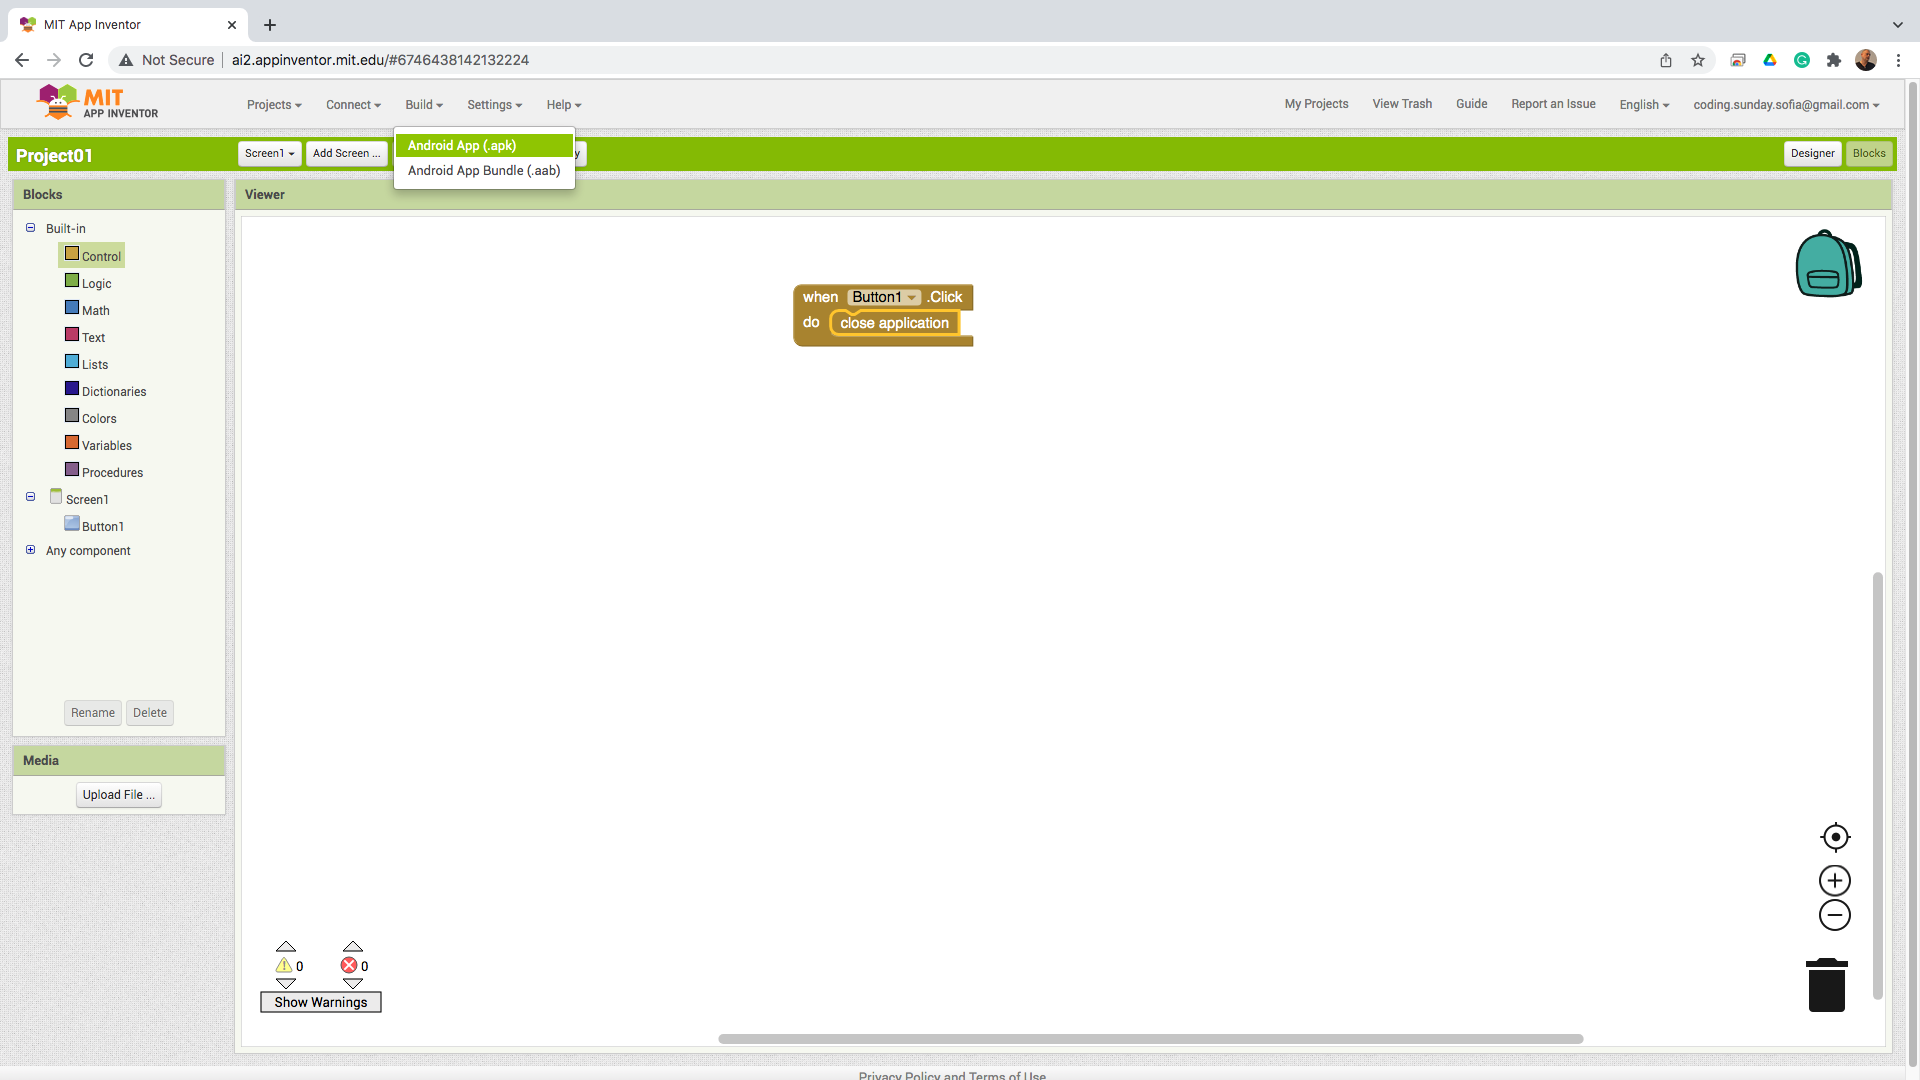
\includegraphics[width=1.0\linewidth,height=0.5\linewidth]{fig010038.png}
   \caption{Mobile App Build Menu}
\label{fig010038}
\end{figure}

One key distinction between Scratch and App Inventor is how the execution of programming instructions is visualized. The result is immediately visible in Scratch within the programming environment's workspace. On the other hand, in App Inventor, the program undergoes a compilation process in the cloud infrastructure, resulting in an installation package that needs to be downloaded and installed on a mobile device. 

Compiling and building the installation package in App Inventor requires a certain amount of computational time, represented by a progress bar (Fig. \ref{fig010039}). This progress bar indicates the ongoing process of converting the visual blocks and program logic into a format that can be installed and executed on a mobile device. The progress bar's length varies depending on the complexity of the program and the computational resources available.

Various optimizations and transformations are applied during the compilation and building process to ensure the program is correctly packaged and ready for deployment. This includes converting the visual components and program logic into the appropriate code the target mobile device can understand and execute.

The visualization of the progress bar serves as a feedback mechanism for users, giving them an estimate of the time required to compile and build the installation package. Once the progress bar is completed, the user can download the installation package and transfer it to their mobile device for installation.

By separating the compilation and installation steps, App Inventor enables users to develop and test their programs within the web-based environment while allowing them to deploy the final application on their mobile devices. This approach provides flexibility and portability, allowing users to create mobile apps that can be shared and used on a broader scale.

\begin{figure}[H]
   \centering
   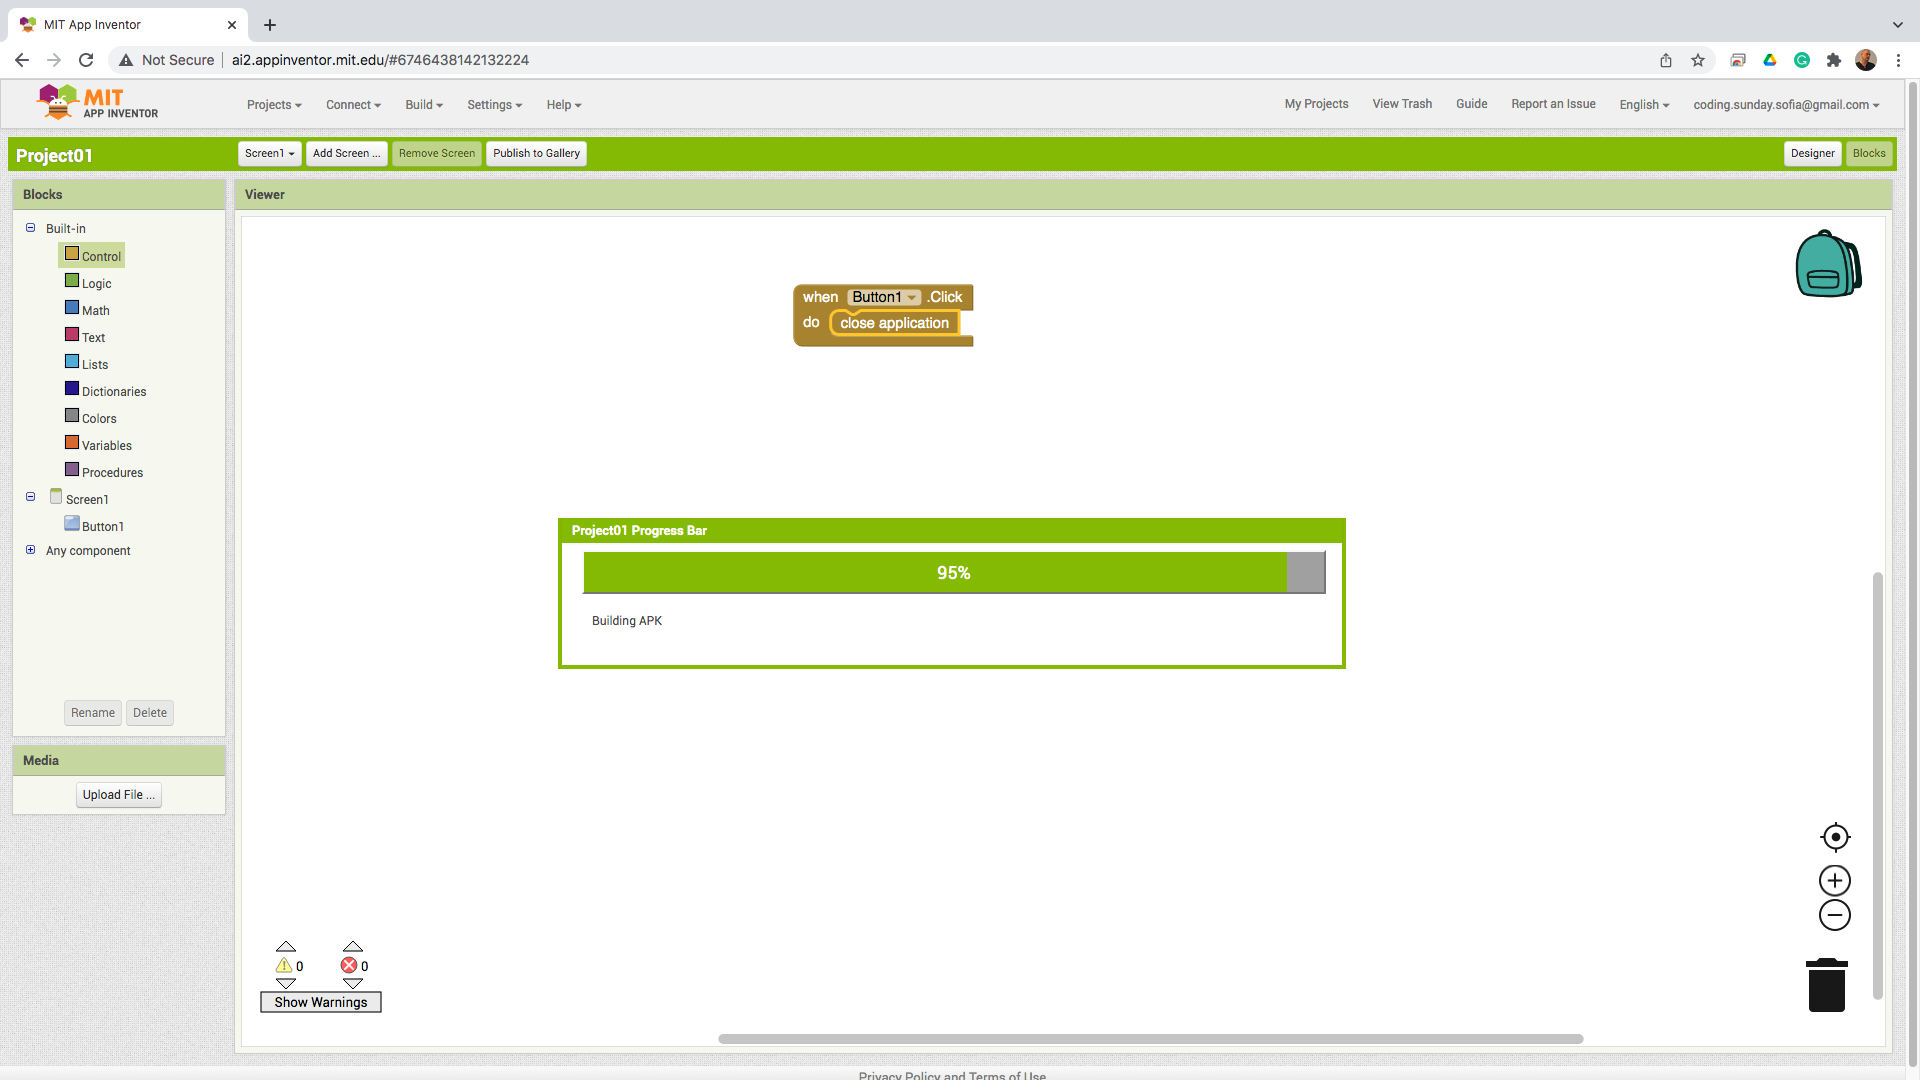
\includegraphics[width=1.0\linewidth,height=0.5\linewidth]{fig010039.png}
   \caption{App build progress}
\label{fig010039}
\end{figure}

Once the project is compiled and the installation package is generated, the programming environment provides a convenient option to download the package onto a mobile device (such as a phone or tablet) using a QR code (Fig. \ref{fig010040}).

A QR code, short for Quick Response code, is a barcode that can be scanned using the camera or a mobile device's dedicated QR code reader app. In the context of App Inventor, the generated QR code acts as a direct link to the installation package, simplifying the process of transferring the app to a mobile device.

To download the app, the user can launch a QR code scanner app or use the built-in camera app on their mobile device to scan the QR code displayed in the programming environment. Upon scanning, the device recognizes the code and prompts the user to download and install the app. This eliminates the need for manual file transfers or complex installation procedures.

The use of QR codes streamlines the distribution and installation process, making it easier for users to access and test their created apps on their mobile devices. It provides a seamless way to bridge the gap between the development environment and the target device, allowing users to experience their apps in a real-world setting.

By leveraging QR codes, App Inventor enhances the convenience and accessibility of deploying apps created within the platform, enabling users to share and showcase their projects with others or use them personally on their mobile devices.

\begin{figure}[H]
   \centering
   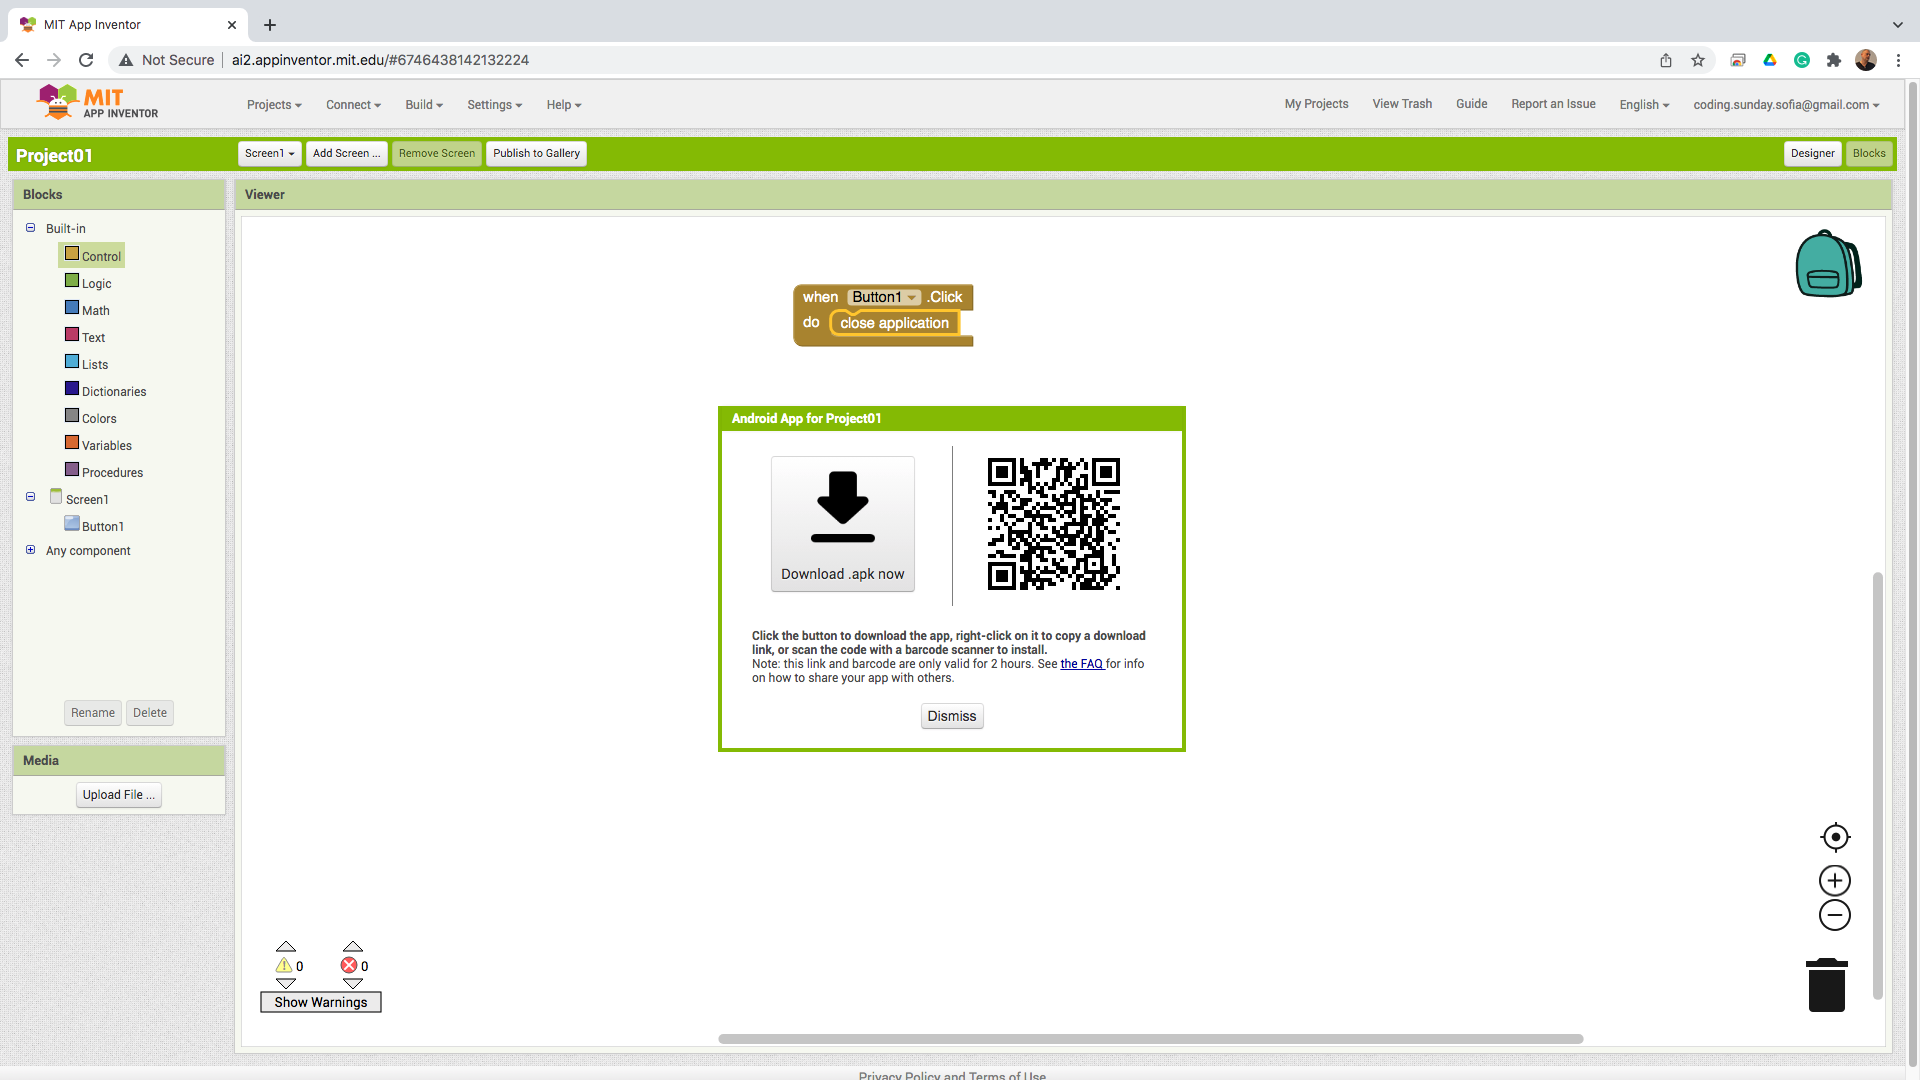
\includegraphics[width=1.0\linewidth,height=0.5\linewidth]{fig010040.png}
   \caption{Code for installing the application on a mobile device}
\label{fig010040}
\end{figure}

The creators of the App Inventor programming environment have developed a dedicated application called MIT AI2 Companion to streamline the installation process of the written programs (Fig. \ref{fig010041}). This application acts as a bridge between the user's mobile device and the cloud infrastructure of App Inventor, facilitating faster and easier testing and deployment of the created apps.

The MIT AI2 Companion app is available for download on Google Play Store and is designed to work seamlessly with App Inventor projects. It eliminates the need for complex manual installations or file transfers by establishing a direct communication channel with the App Inventor cloud infrastructure.

Users can search for and install the MIT AI2 Companion app from Google Play Store onto their mobile devices to utilize this feature. Once installed, they can connect the companion app and their App Inventor projects by scanning a QR code or entering a unique pairing code.

By establishing this connection, the MIT AI2 Companion app allows users to instantly test and run their projects on their mobile devices without complex setup procedures. The app communicates with the cloud infrastructure, enabling real-time synchronization between the development environment and the mobile device.

This approach offers a more streamlined and user-friendly experience, eliminating the need for manual installations or additional technical skills. Users can easily install the MIT AI2 Companion app and leverage its functionality to deploy their projects quickly and efficiently on their mobile devices.

\begin{figure}[H]
   \centering
   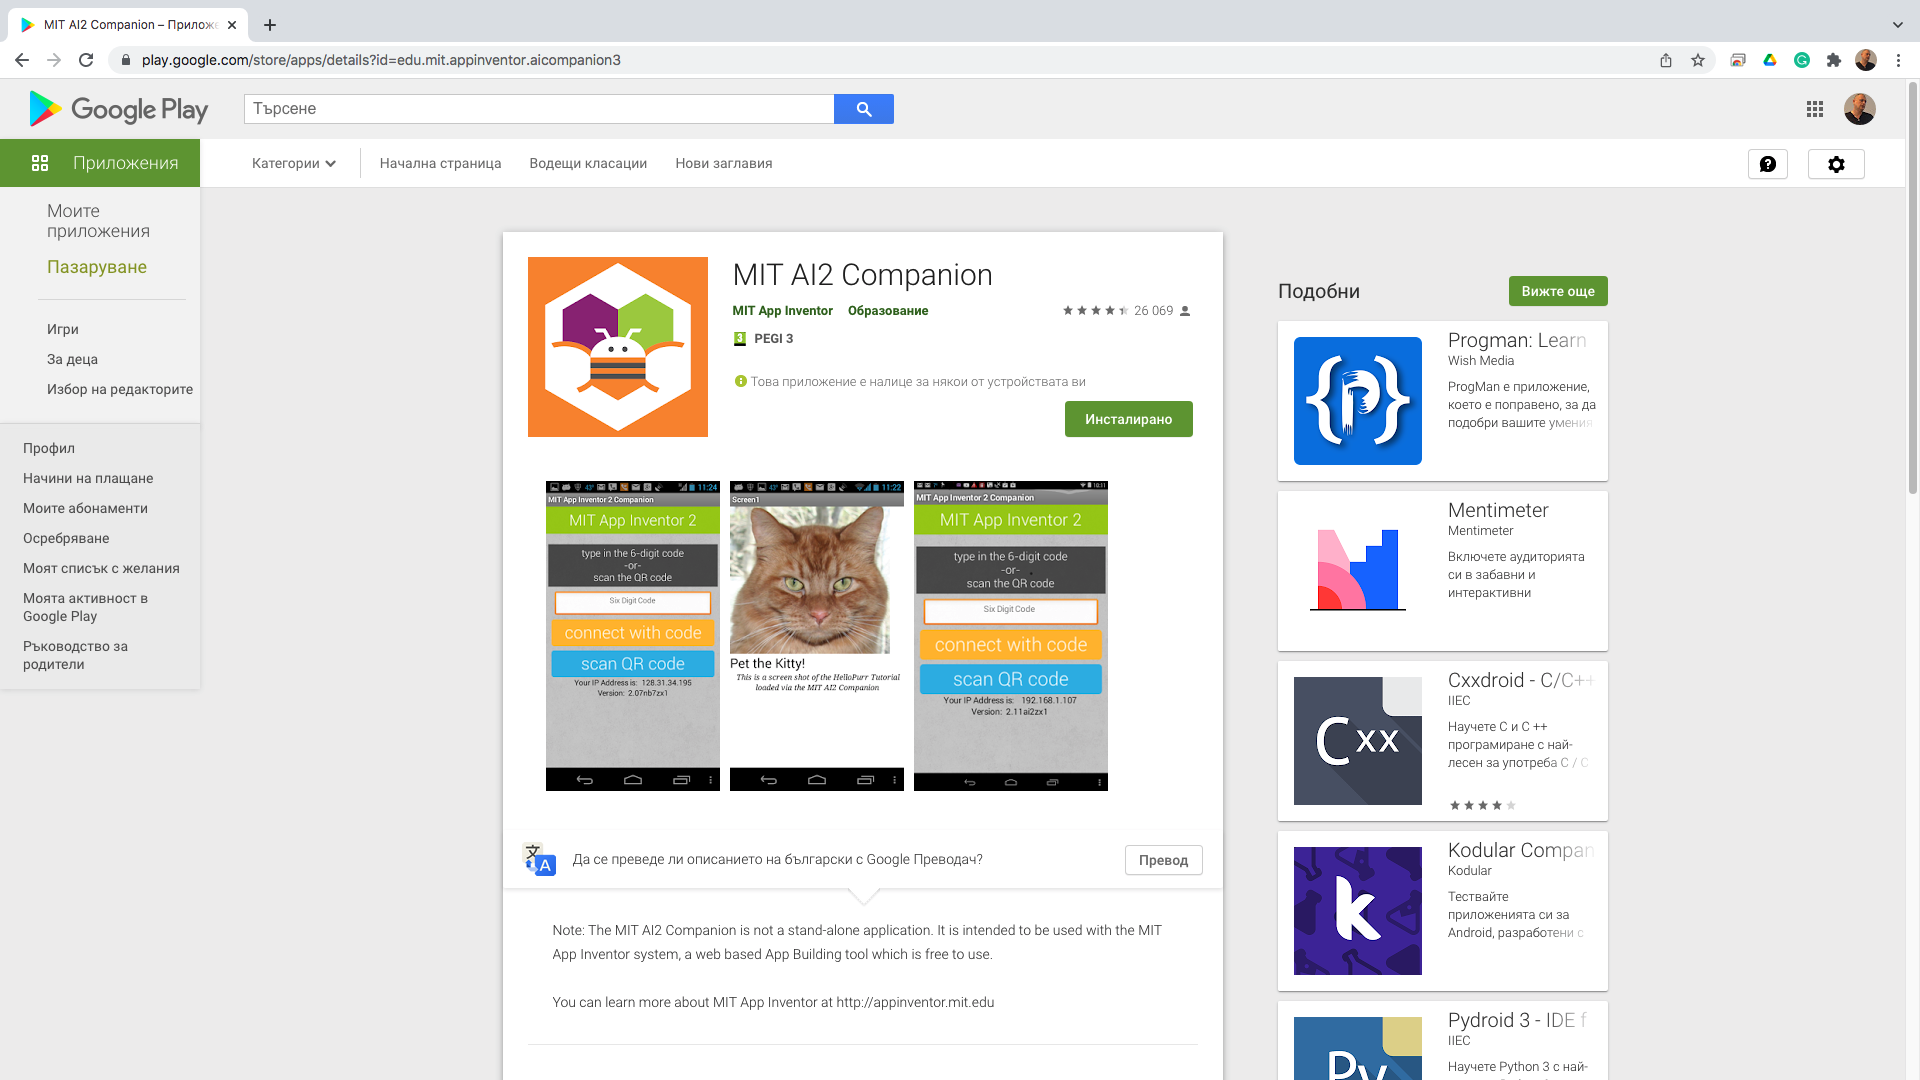
\includegraphics[width=1.0\linewidth,height=0.5\linewidth]{fig010041.png}
   \caption{Mobile application for managing compiled projects}
\label{fig010041}
\end{figure}

When launching the MIT AI2 Companion application, users have two options to download their written programs (Fig. \ref{fig010042}). The first option is to enter a code manually, while the second option is to conveniently scan a QR code (Fig. \ref{fig010043}).

Scanning the QR code provides a faster and more convenient method to initiate the download process. Users can easily capture the QR code associated with their project using the device's camera. This eliminates the need for manual entry and reduces the chance of errors.

However, it's important to note that when downloading the installation package, which is an executable file, the Android operating system may issue a warning (Fig. \ref{fig010044}). This is a standard security precaution, as the system alerts users that such files can be harmful.

To proceed with the download, users can follow the on-screen instructions and confirm their intention to download the file despite the warning. It's essential to ensure that the source of the file is trusted and reliable, such as the App Inventor platform, to minimize any potential risks.

By acknowledging and proceeding past the warning, users can safely download and install the application onto their Android devices, allowing them to run and test their projects seamlessly using the MIT AI2 Companion.

\begin{figure}[H]
   \begin{subfigure}{0.31\textwidth}
   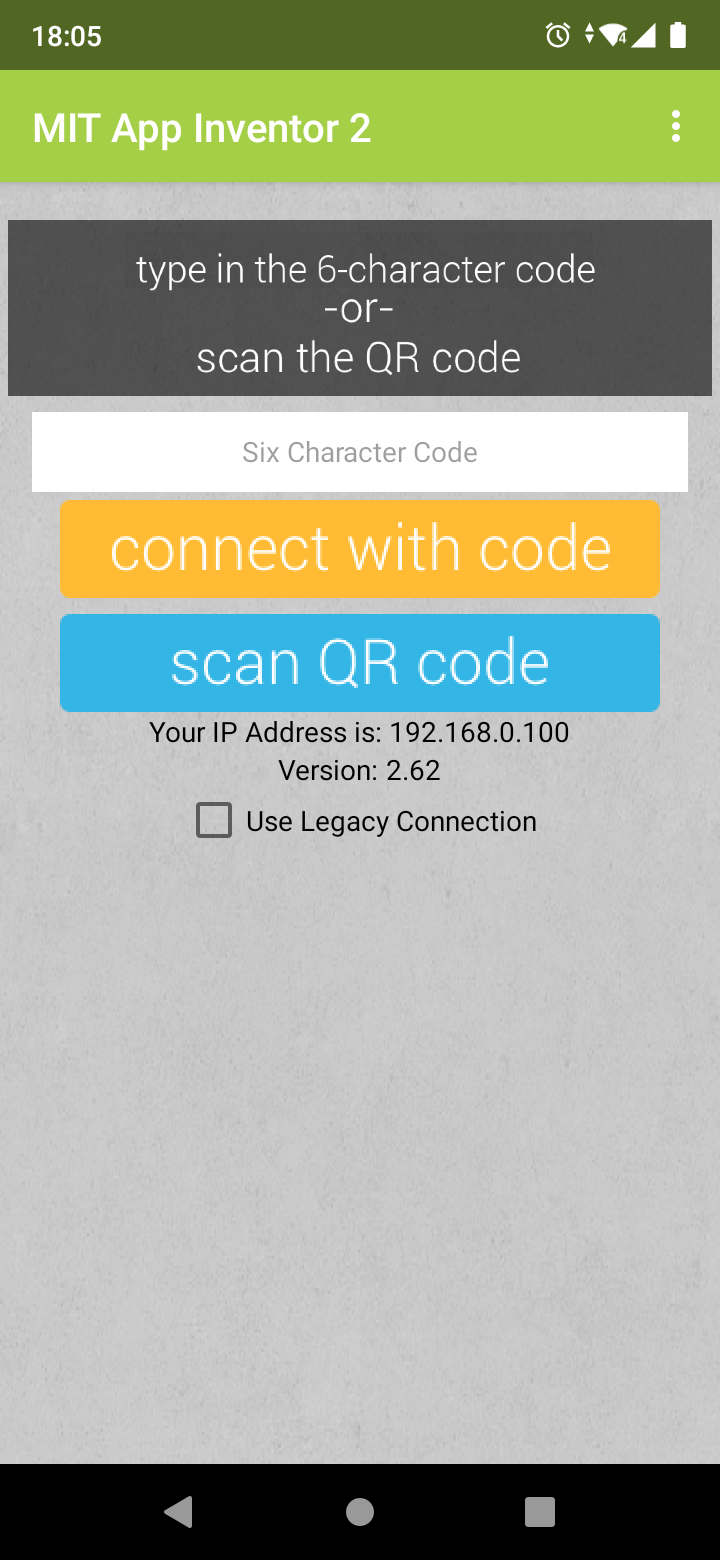
\includegraphics[width=\linewidth]{fig010042.png}
   \subcaption{\tiny Installation Selection}
   \label{fig010042}
   \end{subfigure}
   \begin{subfigure}{0.31\textwidth}
   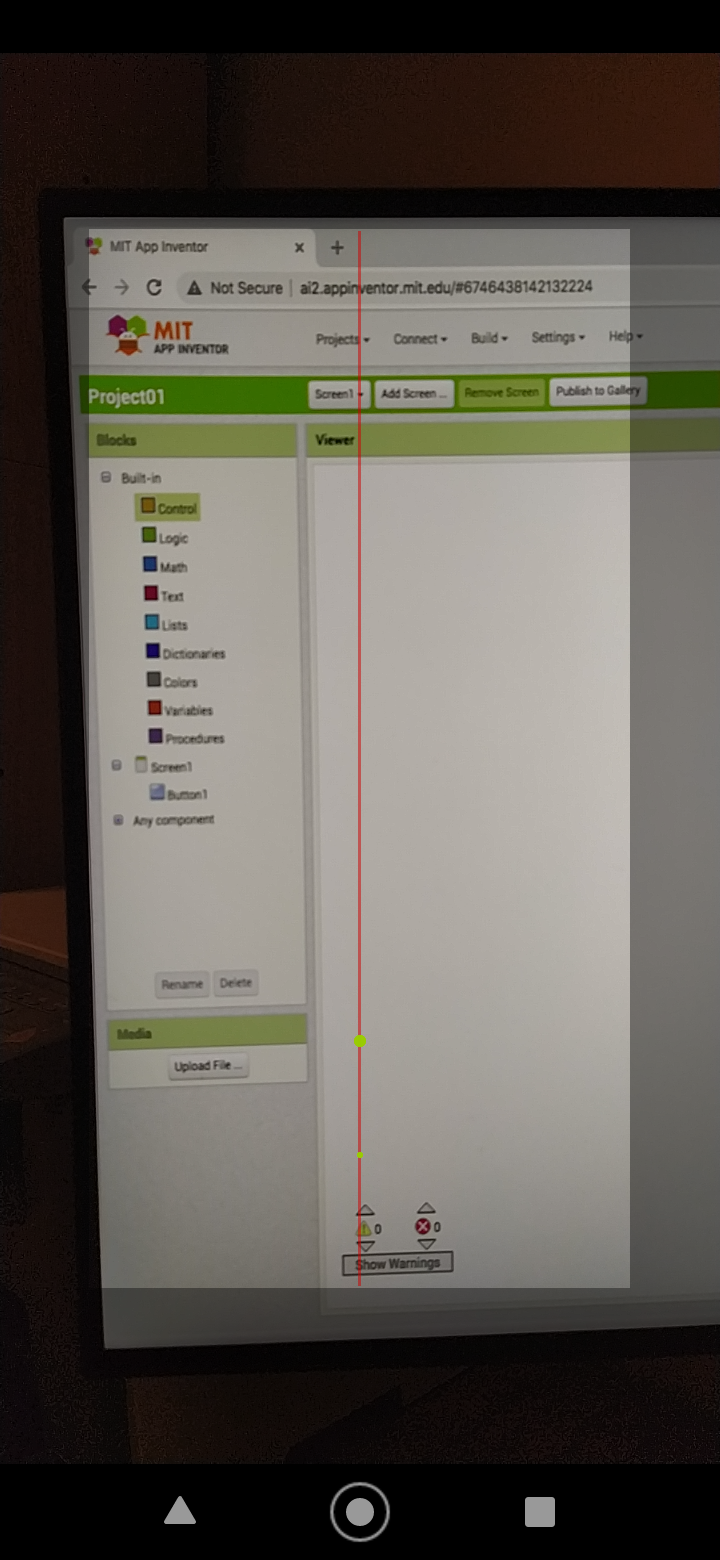
\includegraphics[width=\linewidth]{fig010043.png}
   \subcaption{\tiny Code Scan}
   \label{fig010043}
   \end{subfigure}
   \begin{subfigure}{0.31\textwidth}
   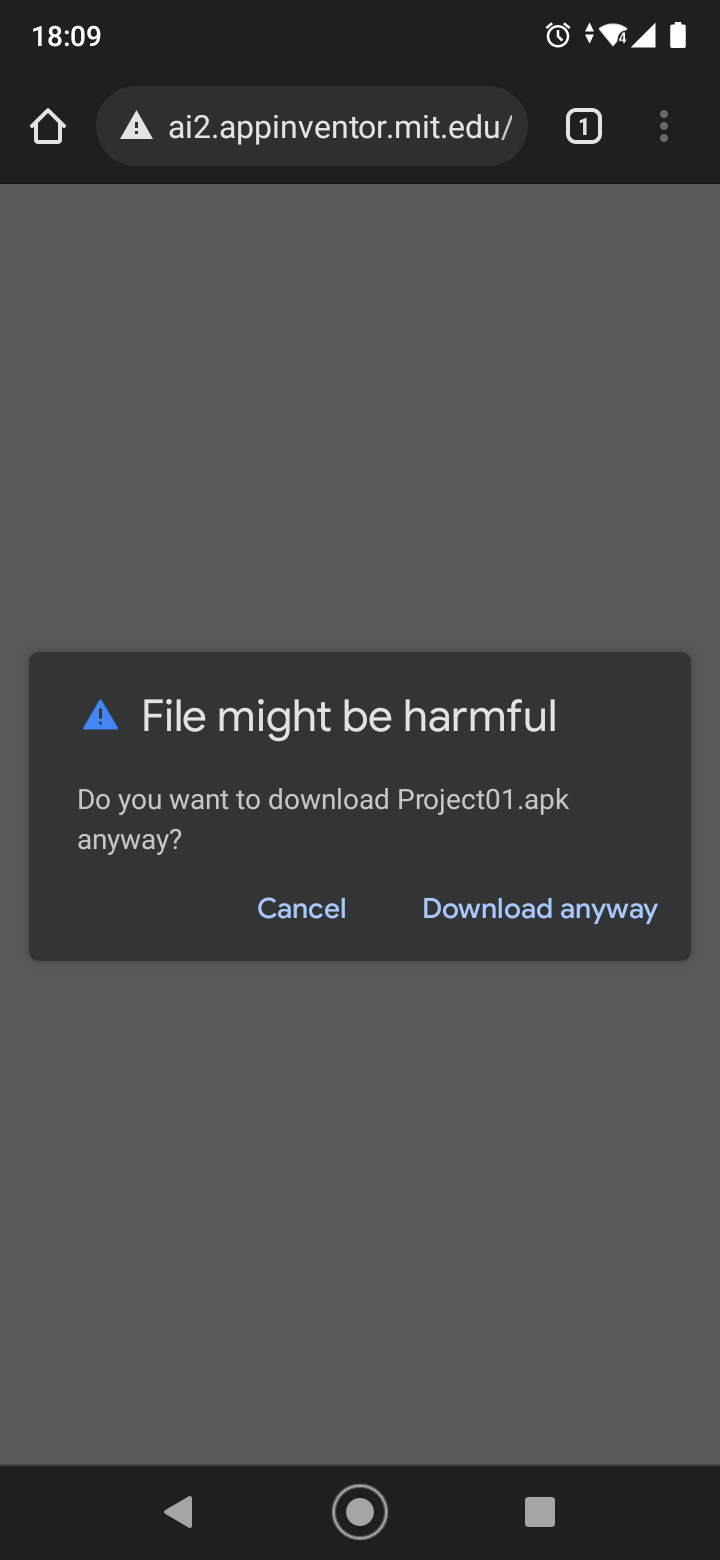
\includegraphics[width=\linewidth]{fig010044.png}
   \subcaption{\tiny Download File}
   \label{fig010044}
   \end{subfigure}
   \caption{Install via QR code}
\end{figure}

After successfully downloading the installation package, the operating system displays a message confirming the successful recording of the installer (Fig. \ref{fig010045}). At this point, the user needs to locate the downloaded installation package and initiate the installation process. Upon selecting the installation package, a prompt appears asking for confirmation to proceed with the program installation contained in the file (Fig. \ref{fig010046}).

It's important to note that even though we know how the installation file was created, the operating system perceives it as a program developed by an unverified developer. As a security measure, the system again prompts the user to confirm their intention to proceed with the installation (Fig. \ref{fig010047}).

This additional confirmation ensures that the user is fully aware of the potential risks of installing applications from unverified sources. By requiring this confirmation, the operating system aims to protect users from potentially harmful or malicious software.

To continue with the installation, the user can confirm their intent by selecting the appropriate option in the prompt. It's recommended to only proceed with the installation if the package's source is trusted and known to be reliable.

Once the user confirms the installation, the operating system will install the program on the device, allowing it to be launched and used as intended.

\begin{figure}[H]
   \begin{subfigure}{0.31\textwidth}
   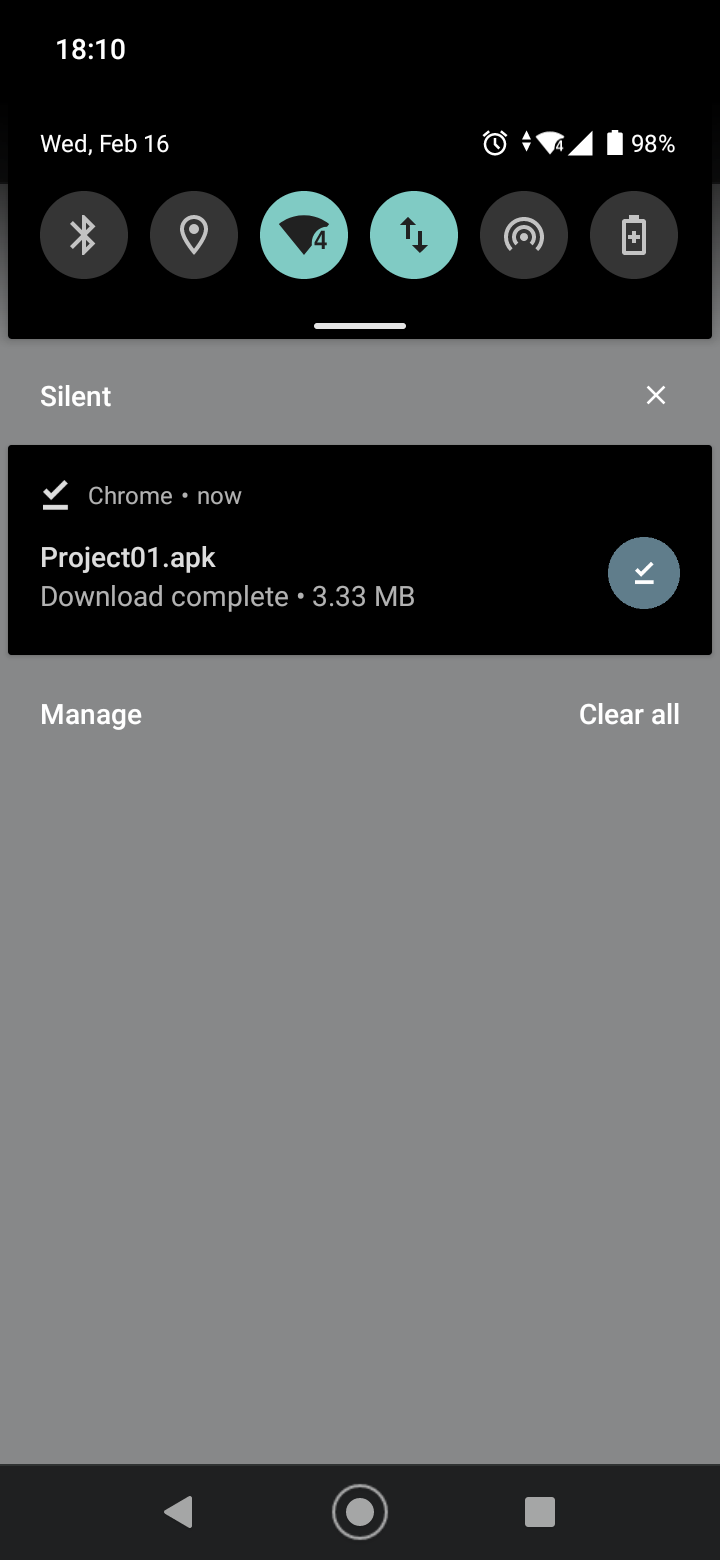
\includegraphics[width=\linewidth]{fig010045.png}
   \subcaption{\tiny File Downloaded}
   \label{fig010045}
   \end{subfigure}
   \begin{subfigure}{0.31\textwidth}
   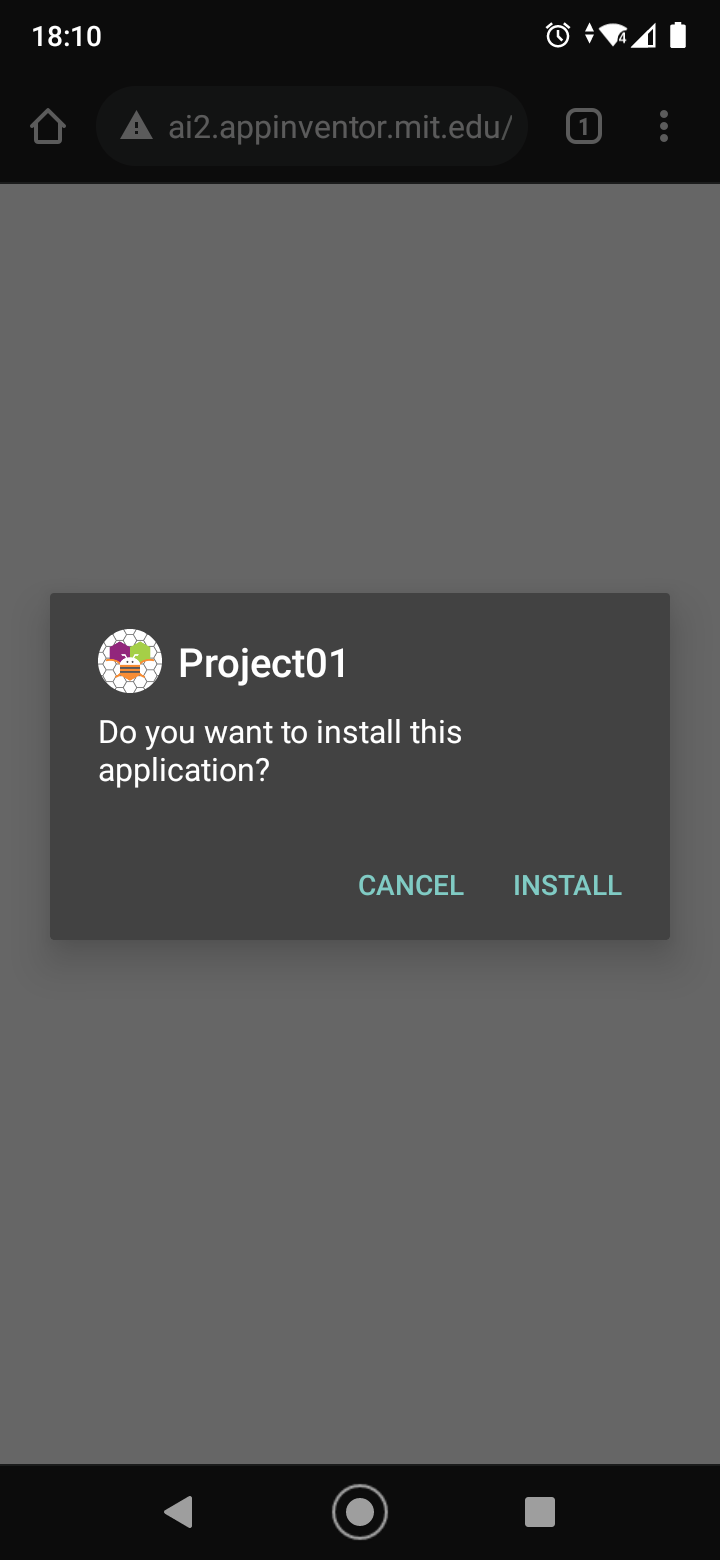
\includegraphics[width=\linewidth]{fig010046.png}
   \subcaption{\tiny Choose to install}
   \label{fig010046}
   \end{subfigure}
   \begin{subfigure}{0.31\textwidth}
   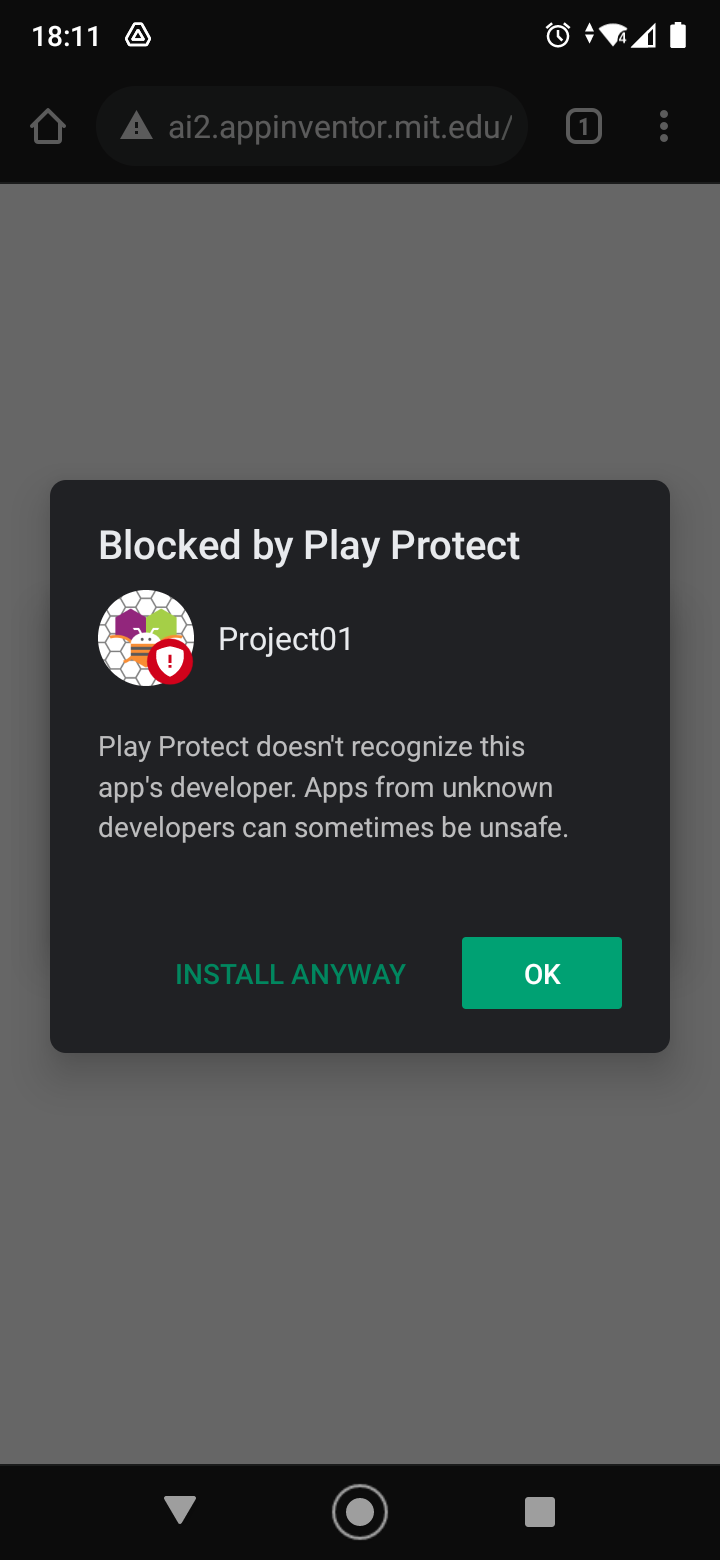
\includegraphics[width=\linewidth]{fig010047.png}
   \subcaption{\tiny Installation Confirmation}
   \label{fig010047}
   \end{subfigure}
   \caption{Installation on the mobile device}
\end{figure}

After selecting "Install Anyway," the written program is successfully installed on the mobile device. The installation process concludes with a window prompting the user to start the newly installed program (Fig. \ref{fig010048}).

To verify the functionality of the written code, press the button displayed in the upper left corner of the application's interface (Fig. \ref{fig010049}). Upon pressing the button, the window will close, and the user will be presented with the virtual wallpaper, indicating that the program is functioning as intended (Fig. \ref{fig010049}).

At this point, the user can interact with the program and experience its intended features and functionalities. It's worth noting that the visualized button triggers the programmed actions, and pressing it initiates the desired behavior or operations within the application.

By following this process, the user can successfully install and execute their written program on their mobile device, allowing them to explore and enjoy the functionality they have created.

\begin{figure}[H]
   \begin{subfigure}{0.31\textwidth}
   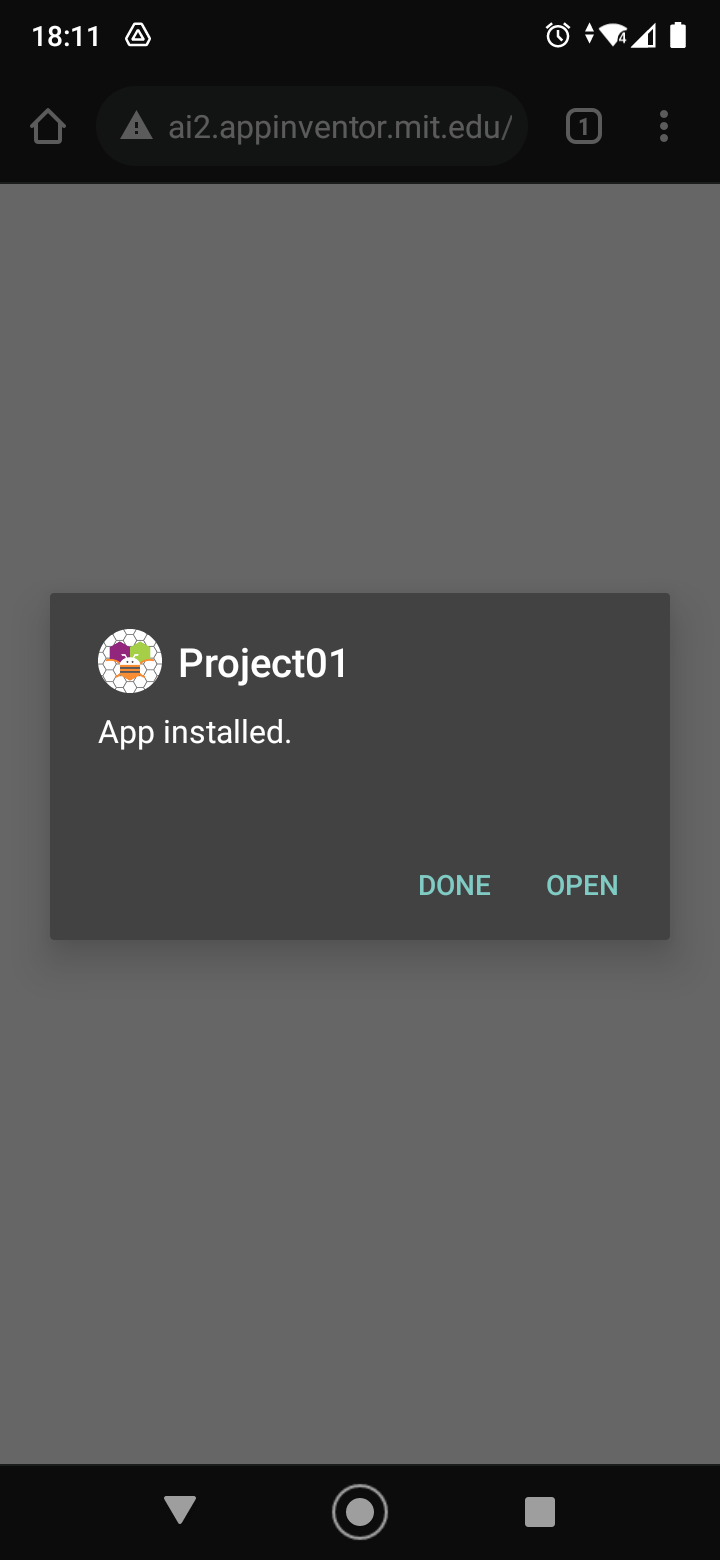
\includegraphics[width=\linewidth]{fig010048.png}
   \subcaption{\tiny Launch}
   \label{fig010048}
   \end{subfigure}
   \begin{subfigure}{0.31\textwidth}
   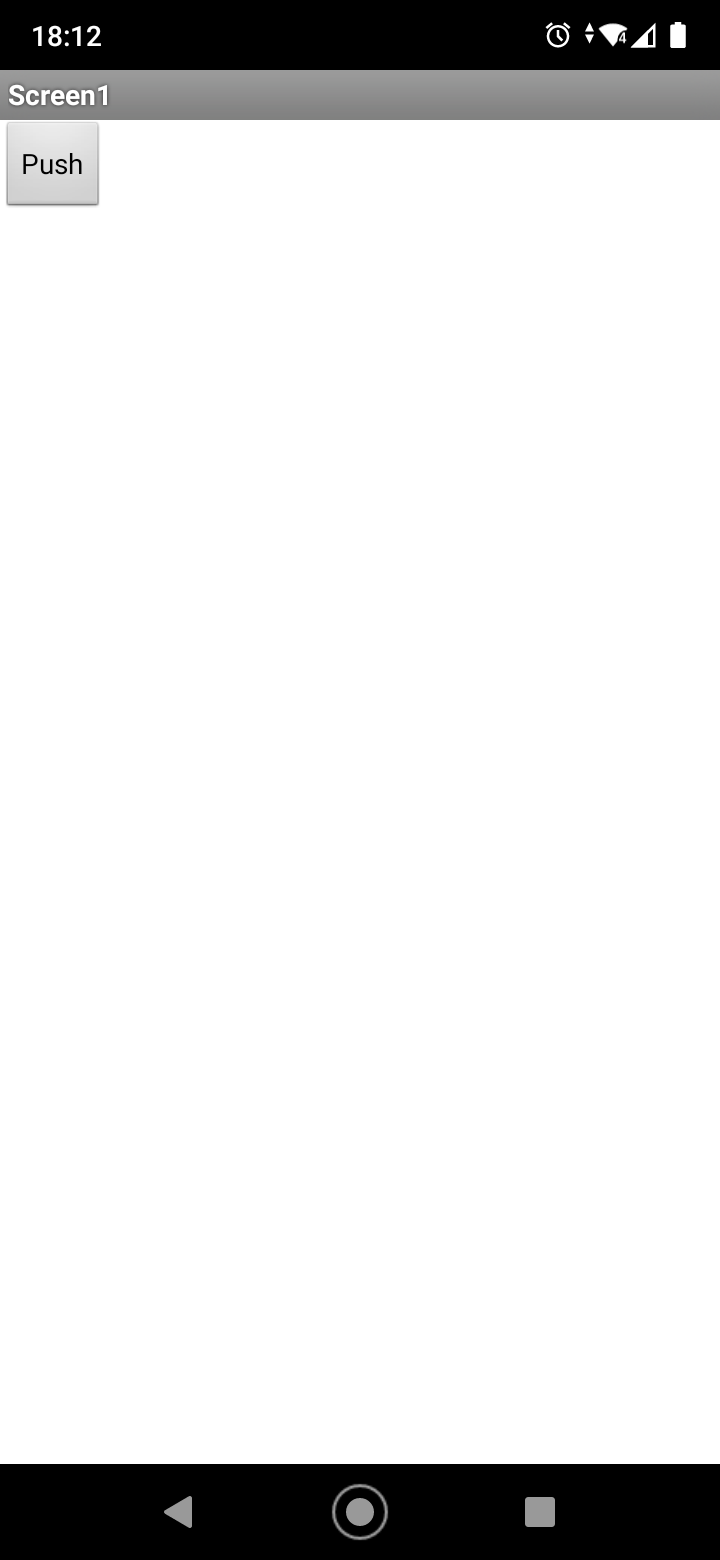
\includegraphics[width=\linewidth]{fig010049.png}
   \subcaption{\tiny Button Selection}
   \label{fig010049}
   \end{subfigure}
   \begin{subfigure}{0.31\textwidth}
   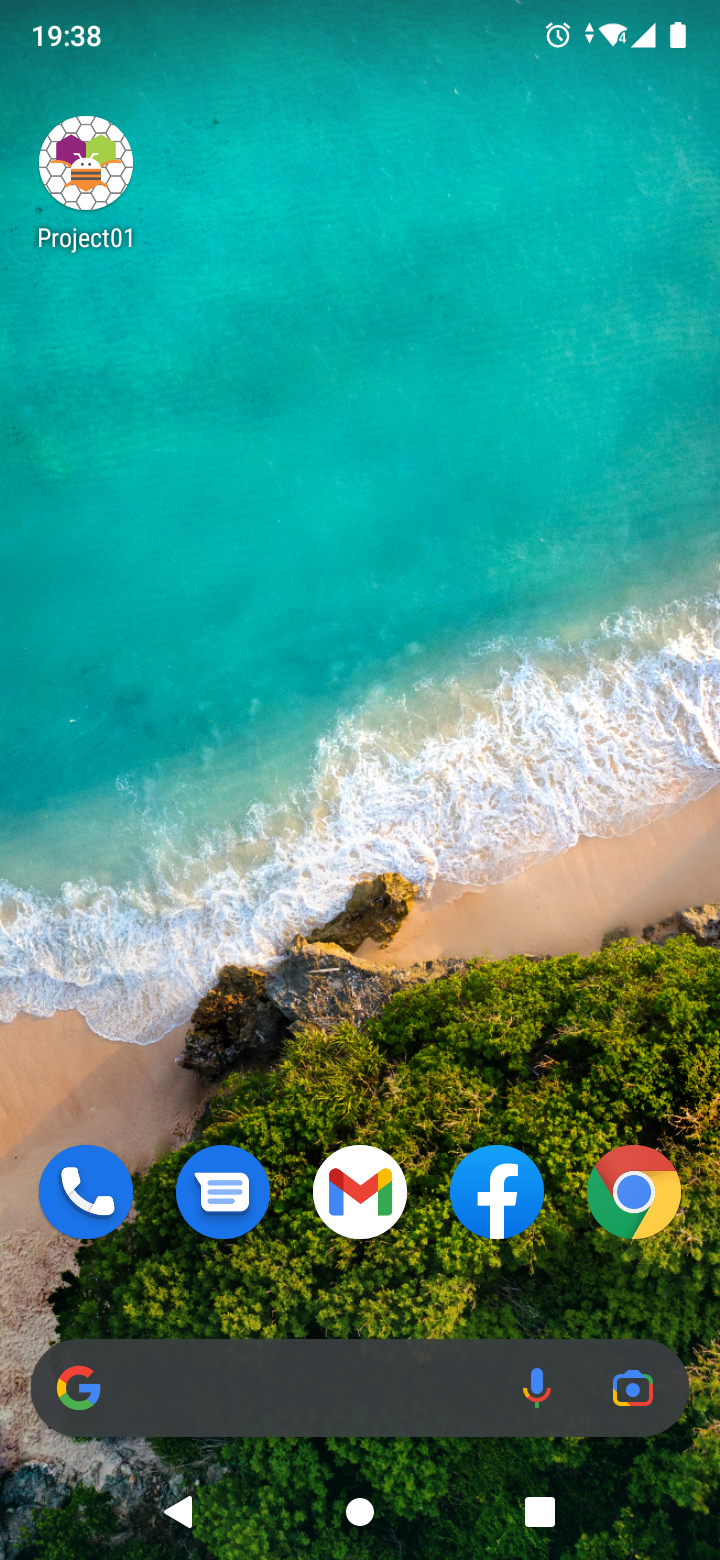
\includegraphics[width=\linewidth]{fig010050.png}
   \subcaption{\tiny Closed App}
   \label{fig010050}
   \end{subfigure}
   \caption{Working with the application}
\end{figure}

App Inventor offers a fascinating aspect - the ability to deploy and showcase developed programs directly on mobile devices. This means that creators can share their work and demonstrate their applications even when away from a computer or without internet connectivity.

This unique feature of App Inventor empowers users to take their creations on the go, allowing them to showcase their programs anytime, anywhere. It opens up possibilities for sharing projects with a broader audience, such as friends, family, or even during presentations or events.

By enabling programs to run on mobile devices, App Inventor brings mobility and accessibility to the forefront, extending the reach and impact of the developed applications beyond traditional computing environments. It adds an exciting dimension to the programming experience, allowing creators to demonstrate their work and engage with users in real-world scenarios.
